\documentclass{article}
\def\lncs{0}
\def\hideobsolete{1}

\usepackage{etoolbox}
\newtoggle{drawfigs}
\togglefalse{drawfigs}
% \toggletrue{drawfigs}


\usepackage{fullpage, amsmath,amsthm,amssymb,graphicx,amsfonts}
\usepackage{authblk}

\usepackage{stix2}
% \usepackage{libertine}



% %\usepackage{thmtools}
% \usepackage{mathtools}
% %\usepackage{thmtools, thm-restate}

% \newtheorem{theorem}{Theorem}
% \newtheorem{claim}{Claim}
% \newtheorem{proposition}{Proposition}
% \newtheorem{lemma}{Lemma}
% \newtheorem{corollary}{Corollary}
% \newtheorem{bound}{Bound}

% \theoremstyle{definition}
% \newtheorem{definition}{Definition}
% \newtheorem{axiom}{Axiom}

% \theoremstyle{remark}
% \newtheorem{fact}{Fact}
% \newtheorem{remark}{Remark}

\usepackage{amsthm,thmtools,mathtools}

% \theoremstyle{plain}
% \newtheorem{theorem}{Theorem}
% \newtheorem{lemma}[theorem]{Lemma}
\declaretheoremstyle[
  notefont=\bfseries, 
  bodyfont=\normalfont\itshape
  %qed=$\diamond$
]{mydef}
\declaretheoremstyle[
  bodyfont=\normalfont\itshape
  % qed=$\diamond$
]{mythm}


\declaretheorem[style=mythm,numberwithin=section]{theorem}
\declaretheorem[style=mythm,sibling=theorem]{lemma}
\declaretheorem[style=mythm,sibling=theorem]{corollary}
\declaretheorem[style=mythm,sibling=theorem]{problem}
\declaretheorem[style=mythm,sibling=theorem]{claim}
\declaretheorem[style=mythm,sibling=theorem]{proposition}
\declaretheorem[style=mythm,sibling=theorem]{fact}
\declaretheorem[style=mythm,name=Claim,numbered=no]{claim*}
\declaretheorem[style=mythm,name=Fact,numbered=no]{fact*}

\declaretheorem[style=mydef,sibling=theorem]{definition}
\declaretheorem[style=definition,qed=$\diamond$]{axiom}
\declaretheorem[style=remark,sibling=theorem]{example}
\declaretheorem[style=remark,sibling=theorem]{remark}




  

%\declaretheorem{theorem}


\usepackage{color}
\usepackage{ifthen}

\long\def\red#1\par{\par\bigskip{\color{red}#1}\par}
\def\showauthnotes{0}

\ifthenelse{\showauthnotes=1}
{
\newcommand{\authnote}[2]{{{[#1: #2]~}}}
}
{ \newcommand{\authnote}[2]{} }

\newcommand{\aggelos}[1]{\authnote{\color{magenta}Aggelos}{#1}}


\newcommand{\InlineCases}[1]{
  \begin{enumerate*}[label=(\textit{\roman*})]
    #1
  \end{enumerate*}
}

\bibliographystyle{plainnat}

% \usepackage{microtype}
\usepackage{amsmath,amsfonts,amssymb}
\usepackage{hyperref}
\usepackage[notrig]{physics}
\usepackage{caption,subcaption}
\usepackage{tikz}
\usetikzlibrary{automata,arrows,positioning,calc}
\usepackage{pgfplots}
\usepackage{subfiles}
\usepackage[numbers,sectionbib]{natbib}
\usepackage[inline]{enumitem}
\usepackage{hhline}
\usepackage{multirow}
\usepackage{framed}
\usepackage{blindtext}

%=========== Commands inherited from the Settlement Time paper ==============
\newcommand\gmargin{\mathbf{m}}
\newcommand{\gf}[1]{\mathsf{#1}}
\newcommand{\hdepth}{\mathbf{d}}
\DeclareMathOperator{\length}{length}
\DeclareMathOperator{\depth}{depth}
\DeclareMathOperator{\height}{height}
\DeclareMathOperator{\gap}{gap}
\DeclareMathOperator{\reach}{reach}
\DeclareMathOperator{\reserve}{reserve}
\DeclareMathOperator{\Divergence}{div}
\DeclareMathOperator{\tdivergence}{tdiv}
\newcommand{\Slot}{\textsl{sl}}
\newcommand{\fprefix}{\sqsubseteq}
\newcommand{\Adversary}{\mathcal{A}}
\newcommand{\Challenger}{\mathcal{C}}
\newcommand{\Honest}{\mathcal{H}}
\newcommand{\Distribution}{\mathcal{D}}
\newcommand{\dominatedby}{\preceq}
\newcommand{\StationaryRho}{\mathcal{R}_\infty}
\newcommand{\DistRho}{\mathcal{R}}
\newcommand{\Union}{\cup}
\newcommand{\Intersect}{\cap}
\newcommand{\BigUnion}{\bigcup}
\newcommand{\BigIntersect}{\bigcap}
\newcommand{\Poly}{\mathsf{poly}}

%-------------------- Commands from the XOR Games -------------
\newcommand{\NN}{\mathbb{N}}
\newcommand{\ZZ}{\mathbb{Z}}
\newcommand{\RR}{\mathbb{R}}
\newcommand{\CC}{\mathbb{C}}

\newcommand{\EpsG}{\mathsf{\varepsilon_g}}
\newcommand{\EpsA}{\mathsf{\varepsilon}_a}
\newcommand{\EpsP}{\mathsf{\varepsilon}_p}
\newcommand{\EpsTotal}{\mathsf{\varepsilon}_{total}}
\newcommand{\gSlice}{\gamma}
\newcommand{\Slice}{\mathsf{slice}}
\newcommand{\Epoch}{\mathsf{epoch}}
\newcommand{\Block}{\mathsf{block}}
\newcommand{\Chain}{\mathcal{C}}
\newcommand{\GameXor}{\mathcal{G}}
\newcommand{\GameNoSynch}{\GameXor_\mathsf{nosynch}}
\newcommand{\GameAllSynch}{\GameXor_\mathsf{allsynch}}
\newcommand{\BlockLength}{\ell}
\newcommand{\EpochLength}{k}
\newcommand{\NumEpochs}{L}
\newcommand{\NonceDim}{\kappa}
\newcommand{\Binomial}{\mathsf{Bin}}
\newcommand{\Poisson}{\mathsf{Poi}}
\newcommand{\Bernoulli}{\mathsf{Ber}}
\newcommand{\Geometric}{\mathsf{Geo}}
\newcommand{\Beacon}{\mathsf{B}}
\newcommand{\Protocol}{\mathsf{P}}


\DeclareMathOperator*{\Exp}{\mathbb{E}}
\DeclareMathOperator*{\Var}{\mathbf{Var}}
\DeclareMathOperator{\wt}{wt}

\pgfplotsset{compat=1.14}

\DeclareRobustCommand{\Eulerian}{\genfrac<>{0pt}{}}
\DeclareMathOperator{\Li}{Li}
\newcommand{\Lifunc}{\Li_{-\lambda}(\alpha)}
\newcommand{\Geom}{\mathcal{G}}
\newcommand{\GeomAlpha}{\Geom_\alpha^+}
\newcommand{\GeomOneMinusAlpha}{\Geom_{1 - \alpha}^+}
% \newcommand{\GeomAlphaHat}{\hat{\Geometric}_\alpha}
\newcommand{\GeomAlphaHat}{\Geom_\alpha}
%\DeclareMathOperator{\Re}{Re}
\newcommand{\defeq}{\triangleq}
\newcommand{\Given}{\mid \,}
\newcommand{\SuchThat}{:}
\newcommand{\EmptyString}{\varepsilon}
% \newcommand{\EmptyString}[1][\kappa]{0^{#1}}
\newcommand{\ZeroString}[1][\kappa]{0^{#1}}
\newcommand{\Z}{\mathcal{Z}}
\newcommand{\DominatedBy}{\preceq}
\newcommand{\MinEntropy}{H_\infty}
\newcommand{\Indicator}{\mathbf{1}}


\newcommand{\Player}{u}
\newcommand{\Players}{\mathcal{U}}
\newcommand{\Leaders}{\mathcal{L}}
\newcommand{\NoncePlayers}{\mathcal{N}}
\newcommand{\Endorser}{E}
\newcommand{\Nonce}{\mathsf{nonce}}
\newcommand{\BeaconProtocol}{\pi_{\mathsf{beacon}}}
\newcommand{\ECQ}{\exists\mathrm{CQ}}
\newcommand{\sECQ}[1][s]{{#1}\text{-}\ECQ}
\newcommand{\CP}{\mathrm{CP}}
\newcommand{\SlotCP}{\CP^{\mathsf{slot}}}
\newcommand{\kSlotCP}[1][k]{{#1}\text{-}\SlotCP}
\newcommand{\Prefix}{\prec}
\newcommand{\PrefixEq}{\preceq}
\newcommand{\Trim}[1]{^{\lceil {#1}}}
\newcommand{\TrimSlot}[1]{\left[1:-{#1}\right]}
\newcommand{\Hrule}{\noindent\rule{\textwidth}{1pt}}
\newcommand{\RandOracle}{\mathsf{H}}
\newcommand{\VRF}{\mathsf{VRF}}
\newcommand{\pk}{\mathsf{pk}}
\newcommand{\sk}{\mathsf{sk}}
\newcommand{\Or}{\text{or,}\quad}
\newcommand{\Blockchain}{\Pi_\mathsf{bc}}
\newcommand{\A}{\mathtt{A}}
\newcommand{\h}{\mathtt{h}}
\newcommand{\Hheavy}{\h\text{-heavy}}
\newcommand{\Aheavy}{\A\text{-heavy}}
\newcommand{\Astar}{\mathtt{A\star}}







%============== Title ================
\title{%Rigorous
  A Decentralized Randomness Beacon with Guaranteed Min-Entropy}

\ifnum\lncs=1
%  \titlerunning{Ouroboros Thoosa}
\fi




%============ Authors ================
\ifnum\lncs=0
  \author[1,4]{Aggelos Kiayias}
  \author[2]{Cristopher Moore}
  \author[3]{Saad Quader}
  \author[3,4]{Alexander Russell}

  \affil[1]{University of Edinburgh}
  \affil[2]{Santa Fe Institute}
  \affil[3]{University of Connecticut}
  \affil[4]{IOHK}

  \else

%  \author{Authors blinded}
% \author{Erica Blum \inst{1}  \and 
%   Aggelos Kiayias \inst{2,5}   \and
%   Cristopher Moore \inst{3}    \and
%   Alexander Russell \inst{4,5} \and
%   Saad Quader \inst{4} 
% }

% \institute{
%   {University of Maryland, College Park}  \and
%   {University of Edinburgh}               \and
%   {Santa Fe Institute}                    \and
%   {University of Connecticut}             \and
%   {IOHK}
% }

\fi


%==================== Begin document ================
\begin{document}
\maketitle

\begin{abstract}
%   We present Ouroboros Thoosa, a Proof-of-Stake (PoS) blockchain protocol with a public leader schedule in the synchronous setting. 
%   It is provably secure against an adaptive adversary in the Universal Composability (UC) framework with Global Setup (GUC). 
  A publicly-verifiable bias-resistant randomness beacon is a fundamental component in many distributed protocols.
  In the first part of our paper, we analyze three schemes for such a beacon that are
  bias-resistant with an overwhelming probability. 
  The adversarial bias in our schemes---called the \emph{grinding power} of the adversary---is 
  defined in a combinatorial sense and it is independent of his computational power. 
  
  Next, we argue that these schemes on top of any distributed protocol which achieves
  \emph{eventual consensus} and \emph{liveness}. 
  Since some provably-secure blockchain protocols satisfy these properties, our scheme can 
  be a drop-in replacement for the randomness beacon in those protocols. 
  This can be attractive for two reasons: 
  (i.) Our scheme is conceptually simpler than some 
  of the existing beacons (e.g., Ouroboros); and 
  (ii.) The security guarantee of many existing protocols [e.g., Ouroboros, Praos, Genesis, GKL, PassShi, and Sleepy] 
  hinge on the assumption 
  that $q$, the number of hashing queries made by the adversary, is polynomial in the security parameter. 
  Our analysis gives an upper bound on $q$ which allows one to choose suitable protocol parameters 
  under which $q$ is indeed bounded by a polynomial in the security parameter.
  
\end{abstract}


% To-Do:
% \begin{enumerate}
% \item Detail the model and connection to blockchain protocols. 
% Consider the 2-player game. 
% \item Introduce a computational method for computing the density. 
% \item Applications: (i) Improving the Common Prefix bound on Ouroboros paper. 
% (can we refine the analysis of the union bound)
% (ii) Providing an exact lower bound on confirmation time for given a certain
% risk level against a double spending attacker that has x amount of stake. 
% \end{enumerate}

% We then provide two rigorous estimates on the basic event of interest---that an adversary can produce a fork that covers a particular portion of a blockchain.

\section{Introduction }

Recall that in Part~\ref{part:praos}, 
we analyzed the randomness beacon in Ouroboros Praos\cite{Praos} and Snow White~\cite{SnowWhite} 
in the synchronous setting. 
We showed 
that the min-entropy loss in the beacon output 
is logarithmic in the security parameter if the adversarial stake is below $9\%$; 
otherwise, it grows linearly in the security parameter.
As Praos is deployed in practice (since August 2020), 
it remains an open question to design simple PoS beacons for Praos 
which can withstand large adversarial stakes.

In this part of the dissertation, 
we present PoS beacons 
whose most salient feature is simplicity and high quality.
In the private leader election setting (e.g., Praos and Snow White), 
our beacon has a superior output quality 
(compared to Praos) 
as long as the adversarial bias is at most $41\%$. 
Although this beacon does not cover adversarial stakes $\alpha$ above $41\%$, 
the regime $\alpha \in (0, 0.41)$ is nonetheless practical: 
for practical values for the consistency parameter $k$, 
Praos' consistency error bound 
starts to degrade when the adversarial stake goes above $40\%$.) 
As an immediate application, it would improve the grinding tolerance in Praos; 
see Figure~\ref{fig:rho-poisson-beacon} for a comparison.

\iftoggle{drawfigs}{

\begin{figure}[!htb]
    \centering
    \tikzsetnextfilename{rho-poisson}
    \begin{tikzpicture}[trim axis left,
      ]
      \begin{axis}[domain=0:1, 
        xmin=0,xmax=1,%,%ymin=-100%,ymax=2.5
        restrict x to domain=0.18:0.99,
        samples=500,
        enlarge x limits=false,
        grid=both,
        no markers, 
        % legend pos=outer north east,
        legend pos=outer north east,
        legend cell align=left,
        x label style={at={(axis description cs:0.5,-0.1)},anchor=north},
        y label style={at={(axis description cs:-0.1,.5)},anchor=south},
        xlabel={$\epsilon$, honest bias},
        title={$\rho^*$, upper bound on the min-entropy loss $\rho$}
        ]
        \addplot +[ultra thick,red] { PraosMinEntropyLossMultiEpoch(\x, 900 ) };
        \addlegendentry{Praos, $k = 900$};
        \addplot +[ultra thick,black] { PoissonBeaconMinEntropyLoss(\x, 900, PraosEpsP(\x, 900)) };
        \addlegendentry{New, $k = 900$};
        \addplot +[ultra thick,blue] { PraosMinEntropyLossMultiEpoch(\x, 1200) };
        \addlegendentry{Praos, $k = 1200$};
        \addplot +[ultra thick,orange,dashed] { PoissonBeaconMinEntropyLoss(\x, 1200, PraosEpsP(\x, 1200)) };
        \addlegendentry{New, $k = 1200$};
      \end{axis}
    \end{tikzpicture}%
    \caption{Min-entropy loss in Poisson beacon}
    \label{fig:rho-poisson-beacon}
\end{figure}

}


We also design a PoS beacon in the public leader election setting 
which can work with Ouroboros classic~\cite{Ouroboros}. 
Recall that Ouroboros classic uses an MPC-based beacon protocol 
which precludes any grinding. 
Implementing this protocol in practice, however, is not palatable. 
We believe that this beacon will be valuable for 
PoS protocols 
that do not have the means to use/implement the MPC-based beacon 
and, in exchange, are willing to tolerate a very low min-entropy loss 
in the beacon. 
See Figure~\ref{fig:rho-bernoulli-beacon}.



\section{A technical overview}
To do



\section{Outline of the exposition}
To do






\section{The security model}
\label{sec:model}


In this \Section, 
we recall the eventual consensus PoS blockchains under the longest-chain rule 
(see \Section~\ref{sec:model-multihonest}). 
% We repeat the necessary components here for the sake of self-containment. 
Recall the consistency property $\kSlotCP$. 
In this section, we introduce a new security property, called the ``Existential Chain Quality Property'' ($\ECQ$), 
which captures the desired behavior that a long enough segment of an honestly held blockchain 
must contain an honest block. 
We use these two properties to define a succinct vocabulary for blockchain security, 
namely, the $(\EpsP, k, s)$-security; this is standard.

Next, we shift our focus toward the leader election schemes. 
Although Praos uses private leader elections, 
we take the opportunity to define the public leader elections as well. 


% \section{Eventual consensus PoS blockchains using the longest-chain rule}
    Let $\Blockchain$ be an eventual consensus PoS blockchain protocol 
    under the longest-chain rule, 
    as in \Section~\ref{sec:model-multihonest}. 
    The protocol $\Blockchain$ advances in discrete rounds 
    which we call \emph{slots}.
    Every participant $u$ in $\Blockchain$ 
    maintains a blockchain $\Chain_u$ 
    and updates it at every slot using the following simple rule: 
    \begin{enumerate}
      \item If a longer blockchain is available in his view, 
      $u$ sets $\Chain_u \leftarrow \Chain$ where 
      $\Chain$ is a longest blockchains. 
      (There could be multiple longest chains.)

      \item If $u$ is assigned to create a block at this slot 
      (i.e., he is a \emph{leader}),
      $u$ adds a new block to $\Chain_u$ and broadcasts immediately.
    \end{enumerate}

    Consider a blockchain $\Chain$ and suppose its most recent block is issued from some slot $s \in \NN$. 
    The ``trimmed chain'' $\Chain\TrimSlot{k}$ is defined as 
    the blockchain obtained from $\Chain$ by deleting all blocks (from $\Chain$) 
    corresponding to the last $k$ slots, i.e., slots $s, s - 1, \ldots, s - k + 1$. 
    In addition, we use the expression $\Chain_1 \Prefix \Chain_2$ to mean that 
    the chain $\Chain_1$ is a prefix of chain $\Chain_2$. 
    Furthermore, given a blockchain $\Chain$ and two slots $t_1$ and $t_2 \geq t_1$, 
    $\Chain[t_1 : t_2]$ denotes the chain segment containing all blocks from $\Chain$ 
    that are issued from slots $t \in [t_1, t_2]$.

    Recall the common prefix property (CP) (in particular, the $\kSlotCP$ property) 
    from Definition~\ref{def:cp-slot-mh}. 
    Below, we mention another important property, 
    the \emph{existential honest chain quality property}: 


    \begin{definition}[Existential Chain Quality property with parameter $s \in \NN$]\label{def:ECQ}        
        Consider slots $t_1, t_2, t$ satisfying $t_1 + s \leq t_2 \leq t$. 
        Let $\Chain$ be the blockchain held by an honest party at slot $t$. 
        Then $\Chain[t_1:t_2]$ contains at least one 
        honestly gneerated block.
    \end{definition}
    We use the shorthand $\sECQ$ for referring to the $\ECQ$ property defined above. 
    Although the analysis of Praos does not contain a proof of this property, 
    the proof should be very similar to the one in Ouroboros Genesis~\cite{Genesis} 
    which is built upon the Praos protocol.
    Next, we can quantify the security of the blockchain protocol in terms of these two properties:

    \begin{definition}[$(\EpsP, k,s)$-security]\label{def:blockchain-security}
        Let $\EpsP \in \RR$ and $k, s \in \NN$. 
        A PoS blockchain protocol is $(\EpsP, k, s)$-secure if 
        it satisfies $\kSlotCP$ and $\sECQ$ property 
        except with probability at most $\EpsP$.
    \end{definition}



\section{Leader election schemes and static/adaptive adversaries}\label{sec:leader-election-public-private}\label{sec:static-dynamic-adversary}

One can consider two types of adversaries in terms of 
how fast they can corrupt an honest player. the so-called \emph{static adversary} 
Suppose that an epoch is $R$ slots long. 
and the \emph{dynamic (or adaptive) adversary}. 
A \emph{static adversary} takes at least $R$ slots to corrupt an honest player 
but an \emph{adaptive adversary} can instantly corrupt an honest player. 
Ouroboros~\cite {Ouroboros} is secure against a static adversary 
while Praos~\cite {Praos} and SnowWhite~\cite{SnowWhite} 
are secure against an adaptive adversary.
The adversarial model critically depends on how a slot-leader is elected. 

Let
$\Players$ be the set of participants 
where each player $i \in \Players$ is associated with a positive real number 
$\sigma_i \in [0,1]$, called his \emph{relative stake ratio}, or just \emph{stake} in short. 
The stake ratios satisfy $\sum_{i \in \Players} \sigma_i = 1$ 
and, for this analysis, remains constant over the course of the execution of the protocol. 
(As is common in the literature (e.g., in \cite{Ouroboros,Praos,SnowWhite}), 
we can handle a change in stake separately from this analysis and then hook these two together.)

Let $\HonestPlayers, \DishonestPlayers \subseteq \Players$ 
denote the set of honest and dishonest players, respectively;
these sets are disjoint and $\Players = \HonestPlayers \Union \DishonestPlayers$.
Given a real $\alpha \in (0,1/2)$, 
we use the notation $\Players(\alpha)$ 
to denote the fact that the total dishonest stake bounded by $\alpha$: i.e., 
$\sum_{i \in \DishonestPlayers} \sigma_i \leq \alpha$
$\sum_{i \in \HonestPlayers} \sigma_i \geq 1 - \alpha$. 
We do not, however, make any assumptions on the number of participants.


In every slot, 
one or more participants are elected as a ``leader'' who can add block to a chain. 
(The claim ``player $u$ won the leader election for slot $i$ at epoch $e$'' 
can be proved using digital signatures and VRFs (Definition~\ref{def:VRF}.)
Let $C_i$ be the set of leaders for slot $i$. 
We consider two types of leader election schemes for an epoch: 
% \begin{enumerate}[label=\textbf{Scheme \Alph*:},ref=\Alph*,leftmargin=3em]
\begin{description}
    \item[\textbf{$\PublicLeaderElection(\alpha)$: Publicly elect a single leader per slot.}] \label{lottery:public}
    At the onset of an epoch, 
    all players use a common random string to 
    publicly sample, 
    independently for each round $i \in [\ell + n]$, 
    a single player $\ell_i \in \Players$ and  
    set $C_i = \{\ell_i\}$. 
    For all players $u \in \Players$, 
    the probability that $u = \ell_i$ is $\sigma_u$. 
    Thus, the leader schedule for an epoch 
    is public knowledge before an epoch commences. 

    \item[\textbf{$\PrivateLeaderElection(\alpha)$: Privately elect zero or more leaders per slot.}] \label{lottery:private}
    Independently for each round $i \in [\ell + n]$, 
    player $u \in \Players$ 
    privately and independently 
    evaluates a Boolean random variable $D$
    which has expectation $\sigma_u$; 
    if $D = 1$, $u$ 
    inserts himself into the set $C_i$ 
    and announces this fact during slot $i$. 
\end{description}
\noindent
Ouroboros uses a public leader election 
at the outset of an epoch 
and, therefore, it is secure only against a static adversary. 
SnowWhtie and Praos (and Bitcoin as well) uses a private leader election 
and therefore, must prove security against an adaptive adversary. 


\section{Praos beacon}\label{sec:praos-beacon-def}\label{sec:praos-model-grindingpower-minentropy}
The Praos blockchain protocol $\Blockchain$ 
proceeds in epochs $t = 1, 2, \ldots$. 
An epoch is long enough 
so that after it is complete, 
the first $n$ slots become settled 
(in the sense of $\kSlotCP$).


\begin{definition}[Praos beacon with parameter $\kappa, n \in \NN$]\label{def:praos-beacon}
  Let $\eta_0 \in \{0,1\}^\kappa$ be a uniformly random string, known to all participants 
  at the outset of the protocol.
  After each epoch $t$, 
  a \emph{beacon output} $\eta_t \in \{0,1\}^\kappa$ is computed, as follows: 
  % which takes a ``seed'' $\eta_{e-1} \UniformIn \{0,1\}^\kappa$ 
  % as input and outputs a string $\eta_e \in \{0,1\}^\kappa$, as follows:
  \begin{enumerate}
    \item $\eta_{t-1}$ is called the \emph{initial value} for epoch $t$.

    \item Every new block added during slots $i \in [n]$ in an epoch contains 
    a uniformly random Boolean string of length $\kappa$; 
    it is called a \emph{nonce}.

    \item Let $u$ be an honest observer at the onset of the next epoch. 
    He computes the beacon output for this epoch, $\eta_t$, 
    by XORing all nonces recorded in his blockchain 
    along with $\eta_{t-1}$ 
    and then applying to it a cryptographic hash function.
  \end{enumerate}
  Note that the consistency property of the blockchain 
  would ensure that all honestly-held blockchains 
  at the onset of epoch $e + 1$ 
  will agree about the blocks issued from 
  the first $n$ slots of epoch $e$.  
\end{definition}

% The length of each epoch is $R \geq n + k$. 

% \begin{definition}[Praos beacon with dimension $\kappa$]\label{def:praos-beacon}~
%   \begin{itemize}
%     \item Before the protocol commences, 
%     all participants are given a uniformly random string $\eta_0 \in \{0,\}^k$. 

%     \item Before epoch $t = 1, 2, \ldots$ commences, 
%     a string $\eta_{t-1}$ is given to all players; 
%     this is called the \emph{initial value} for this epoch. 
%     In fact, for $t \geq 2$, $\eta_{t-1}$ is the beacon output from the previous epoch; see below.

%     \item Inside slot $i$ in epoch $t$, 
%     when a slot leader $u$ issues a new block, 
%     he also includes a \emph{nonce input} 
%     $\VRF_{\PrivateKey(u)}(t \Vert i \Vert \eta_{t-1}) \in \{0,1\}^\kappa$. 
%     Here, $\Vert$ denotes concatenation.
    
%     \item After the epoch is complete, 
%     every honest participant computes the beacon output $\eta_t \in \{0,1\}^\kappa$ as follows: 
%     he gathers all nonce inputs 
%     from a specified prefix of his blockchain, 
%     XORs them together, and then applies a cryptographic hash.
%   \end{itemize}
%   The strings $\eta_1, \eta_2, \ldots$ are called the beacon outputs.
% \end{definition}

The common, public random string $\eta_{t-1}$ 
is used in various computations in epoch $t$, 
including the leader election process.

Specifically, $\eta_{t-1}$ is used by all participants in epoch $t$ 
(in combination with their respective private keys) 
to randomly select a player-specific VRF (see below) 
and use it to elect leaders from among themselves.
Therefore, the ``randomness''
of $\eta_1, \eta_2, \ldots$ is critical factor underlying 
the security of the blockchain protocol; 
we explore this next.

\Paragraph{Beacon output quality.}
Let $n \in \NN$ and let $A$ be the set of $n$-bit Boolean strings.
Suppose a random variable $X$ takes values from $A$
and its probability distribution is $\mathcal{X}$. 
One way to measure how ``random'' the outcomes of $X$ are 
is to measure the \emph{min-entropy} of $X$:

\begin{definition}[Entropy and Min-entropy]
    Let $X$ be a random variable (taking values from set $A$) 
    and let $\mathcal{X} : A \rightarrow [0,1]$ be its probability distribution.
    The \emph{entropy} of $X$ is defined as 
    \begin{equation}\label{def:entropy}
        H(X) = \sum_{x \in A} \mathcal{X}(x) \log_2 (1/\mathcal{X}(x))
        \,.
    \end{equation}
    The \emph{min-entropy} of $X$ is defined as 
    \begin{equation}\label{def:min-entropy}
        H_\infty(X) = - \log_2 \max_{x \in A} \mathcal{X}(x)
        \,.
    \end{equation}
    We also write $H_\infty(\mathcal{X})$ to denote the min-entropy of $X$.
\end{definition}
\noindent

In the above definition, 
if $A = \{0,1\}$ and $X$ is a Boolean random variable with expectation $\alpha \in (0,1)$, 
the entropy of $X$ is given by 
the \emph{binary entropy function} $H: [0,1] \rightarrow [0,1]$ defined as 
\begin{align}\label{eq:binary-entropy}
    H(\alpha) &= -\alpha \log_2(\alpha) - (1-\alpha) \log_2(1-\alpha)
\end{align}
where, By convention, we set $H(0) = H(1) = 0$. 
Since $H$ is a linear combination of logarithms, it is concave. 

Let $U$ be a uniformly distributed random variable on $A$; 
notice that $H_\infty(X) \leq H_\infty(U) = \log_2(|A|)$. 
If $X$ has a low min-entropy, 
it indicates that the distribution of $X$ is ``far'' from being uniformly random. 
Specifically, \emph{the min-entropy loss in $X$} 
is defined as the difference between $H_\infty(X)$ and $H_\infty(U) = \log_2(|A|)$.


\Paragraph{Grinding power and beacon security}
Let $n \in \NN$ and $A \subseteq \{0,1\}^n$.
Let $\eta_0$ be uniformly random in $\{0,1\}^n$ 
and it is used as the initial value for the beacon protocol. 
Let $X_t \in A$ be the random variable 
representing the beacon output at epoch $t$, 
i.e., $X_t = \eta_t, t \in 1, 2, \ldots$\,. 
Let $\mathcal{X}_t$ be the distribution of $X_t$. 

\begin{definition}[Grinding power, informal]\label{def:grinding-power-num-choices}
The \emph{grinding power} $g$ of the adversary $\Adversary$ 
for the beacon output $\eta$
is the number of choices $\Adversary$ has for $\eta$. 
The grinding power of $\Adversary$ over 
the lifetime of the beacon protocol
is the maximum over all beacon outputs.
\end{definition}

Consider a simple one-round game played by the adversary $\Adversary$. 
Assume that $\Adversary$ has a \emph{target} $\eta^* \in \{0,1\}^n$. 
$\Adversary$ wins if $X = \eta^*$; he loses otherwise. 
Let $p_\Adversary$ be his winning probability. 
If $X$ were uniform in $\{0,1\}^n$, 
$p_\Adversary$ would have been $2^{-n}$. 
If the grinding power $g$ is larger than one, 
$X$ is not uniform since 
$\Adversary$ can reset it $g$ times 
and inflate his winning probability to $g 2^{-n}$. 
Thus, 
$$ 
    \max_{\eta \in \{0,1\}^n} \mathcal{X}(\eta) \geq \mathcal{X}(\eta^*) = g 2^{-n}
$$ 
and, consequently, 
$$
    H_\infty(X) \geq -\log_2 (g 2^{-n}) = n - \log_2 g
    \,.
$$
Thus, we have proved the following fact:

\begin{fact}\label{fact:min-entropy-grinding-power}
  For any beacon with grinding power $g$, 
  the min-entropy loss in its output is at most $\log_2 g$.
\end{fact}

\begin{definition}[Beacon security]\label{def:beacon-security}
    Let $n,k,s \in \NN, \rho \in \RR_+$ and $\EpsP, \EpsG \in (0,1)$.
    Let $\Pi_\Beacon$ be a beacon protocol for $n$-bit Boolean strings 
    used in conjunction with a blockchain protocol $\Pi$. 
    Let $\mathcal{B}$ be the distribution of the beacon output.
    Let $E$ be the event that $\Pi$ remains $(\EpsP, k, s)$-secure over the lifetime of the protocol. 
    Condition on $E$. 
    Suppose that except with probability $\EpsG$, 
    the (conditional) min-entropy 
    $H_\infty(\mathcal{B} \mid E)$ is at least $n - \rho$. 
    Then we say that $\Pi_\Beacon$ is \emph{$(\EpsP + \EpsG, \rho)$-secure}.
\end{definition}



Note that the output of the beacon at epoch $L = 2, 3, \ldots$  
is a sequential composition of $L$ independent instances of $\Pi_\Beacon$; 
the output from an epoch is used as the initial value for the next epoch. 
Specifically, 
the beacon output for epoch $t \in [L]$ is 
\begin{align}\label{eq:beacon-iterated}
    \eta_t = \Pi_\Beacon(\eta_{t-1}) = \Pi_\Beacon^t(\eta_0)\,.
\end{align}
where $\eta_0$ is the uniformly random initial value for the first epoch 
and the superscript $t$ denotes a $t$-fold sequential composition.


\begin{lemma}[Security, iterated beacon]\label{lemma:beacon-composition}
Let $\EpsP \in (0,1)$ and $\rho \in \RR_+$.
Suppose $\Pi_\Beacon$ remains $(\EpsP, \rho)$-secure over a single epoch. 
When it is iterated $L$ times as in~\eqref{eq:beacon-iterated}, 
it remains $\left(L 2^\rho \EpsP, \rho\right)$-secure 
over the $L$ epochs.
\end{lemma}
\begin{proof}
    Let $\Pi_t$ be the instance of $\Pi_\Beacon$ at epoch $t$. 
    We will prove the claim by an induction on $t \in [L]$. 

    Each protocol instance $\Pi_t, t \in [L]$ 
    is an independent instance of $\Pi_\Beacon$. 
    Our inductive hypothesis is that for $t \in [L]$, 
    all previous instances 
    $\Pi_\tau, \tau \in [t-1]$ remain $(\EpsP, \rho)$-secure in epoch $\tau$. 
    Thus, there are at most $2^\rho$ choices for $\eta_{t - 1}$, 
    resulting from the grinding in epoch $t-1$.
    By a union bound on these choices, $\Pi_t$ is $(2^\rho \EpsP, \rho)$-secure. 
    A union bound over $t \in [L]$ shows that 
    except with probability at most $L\cdot 2^\rho \EpsP$, 
    every $\Pi_t, t \in [L]$ is $(2^\rho \EpsP, \rho)$-secure.
\end{proof}


In \Section~\ref{sec:praos}, we characterize the grinding power 
for the beacon protocol of Ouroboros Praos~\cite{Praos} and Snow White~\cite{SnowWhite}.
We end the current section by giving a definition of VRF.

\newcommand{\Gen}{\mathsf{gen}}
\newcommand{\Prove}{\mathsf{prove}}
\newcommand{\Verify}{\mathsf{verify}}
% \newcommand{\pk}{\mathsf{pk}}
% \newcommand{\sk}{\mathsf{sk}}
\begin{definition}[Verifiable Random Function (VRF)]\label{def:VRF}
  A family $\mathcal{F}$ 
  of functions $F : \{0,1\}^\ell \rightarrow \{0,\}^k$ 
  is a family of VRFs if there exist algorithms 
  $(\Gen, \Prove, \Verify)$ 
  so that the following holds: 
  $\Gen(1^k)$ outputs a pair of keys $(\pk, \sk)$; 
  $\Prove_\sk(x)$ outputs a pair $(F_\sk(x), \pi_\sk(x))$ 
  where 
  $F_\sk \in \mathcal{F}$, $F_\sk(x)$ is the function value, and 
  $\pi_\sk(x)$ is the proof of correctness; and 
  $\Verify_\pk(x,y,\pi_\sk(x))$ efficiently verifies 
  that $y = F_\sk(x)$ using the proof $\pi_\sk(x)$, 
  outputting 1 if $y$ is valid and 0 otherwise. 
  Additionally, we require the following properties:

  \begin{enumerate}
    \item \emph{Uniqueness:} 
    No values $(\pk, x, y, y', \pi, \pi')$  can satisfy both 
    $\Verify_\pk(x,y,\pi) = 1$ and $\Verify_\pk(x,y',\pi') = 1$ 
    unless $y = y'$.

    \item \emph{Provability:} 
    If $(y, \pi) = \Prove_\sk(x)$ then $\Verify_\pk(x,y, \pi) = 1$.

    \item \emph{Pseudorandomness:} 
    To all probabilistic polynomial-time (PPT) algorithm 
    which runs $\Poly(k)$ steps when its first input is $1^k$ 
    and does not query the $\Prove$ oracle on $x$, 
    the distribution of $F_\sk(x)$ appears uniform in $\{0,1\}^k$, 
    except with a probability negligible in $k$.
  \end{enumerate}

\end{definition}






% \section{Definitions}
% \label{sec:definitions}
% As we have outlined before, 
if slot $t$ in a characteristic string $w$ 
has the Unique Vertex Property (UVP) 
then the slots $s = 1, \ldots, t$ 
are settled in every fork for $w$. 
Our current goal is to 
characterize when a slot has the UVP. 
(In \Section~\ref{sec:fork-framework}, we show an alternative way 
to characterize the UVP; see Lemma~\ref{lemma:uvp-margin}.) 
% When the symbols in $w$ are independent and identically distributed, 
% this alternate characterization allows us to explicitly compute 
% the probability that a given slot has the UVP in $w$.)

We start with laying down some structural properties of forks. 
Next, we define the so-called Catalan slots 
and show that if a slot is Catalan then \emph{in every fork}, all sufficiently long blockchains must contain a block from that slot. 
Next, we show that this implication is actually an equivalence. 
Finally, 
we revisit the above implication assuming 
that the honest players use a consistent longest-chain tie-breaking rule.





%%% Local Variables:
%%% mode: latex
%%% TeX-master: "main"
%%% End:


% \pagebreak         
\section{Coin-flipping in PoS blockchains with the longest-chain rule}
\label{sec:grinding-praos}


Let $\kappa, n \in \NN$. 
Recall the Praos beacon with parameters $\kappa$ and $n$ from Definition~\ref{def:praos-beacon}. 
The goal of this \Section is to state our main results 
about the quality of the Praos beacon 
in terms of its min-entropy after multiple epochs (Definition~\ref{def:beacon-security}).

As we have done in the modeling of the consistency problem 
(\Section~\ref{sec:model-multihonest}), 
we start by defining the so-called ``characteristic string'' $w$. 
It captures the outcomes of the private leader election process $\PrivateLeaderElection$ 
in these slots. 
Next, we use the definition of the Praos beacon protocol to 
derive an expression for its grinding power on $w$.
Next, for some $\epsilon \in (0,1)$, 
we define a distribution $\mathcal{L}((1-\epsilon)/2)$ on the set of characteristic strings of length $n$; 
this represents the outcome of $\PrivateLeaderElection((1-\epsilon)/2)$, i.e., 
a private leader election with an adversarial stake-minority.
We finish this \Section by stating our main theorem about the min-entropy loss in the Praos beacon. 
The proof of this theorem is presented in \Section~\ref{sec:praos-second-moment}.




% \newcommand{\Suffix}[2]{ {#1}^{\overset{#2}{\leftarrow} } }
% \newcommand{\Suffix}[2]{ {#1}[-{#2}:] }
\newcommand{\Suffix}[2]{ \mathsf{suffix}({#1},{#2})}
\newcommand{\CoinTossingLC}{\Pi_\mathsf{lc}^{\Players(\alpha),k,n}}



% Let $\EpsP \in (0,1)$ and $s, k \in \NN$. 
% Let $\Blockchain$ be an $(\EpsP, k, s)$-secure eventual consensus PoS blockchain protocol 
% under the longest-chain rule, such as 
% Ouroboros Praos~\cite{Praos} and Snow White~\cite{SnowWhite}. 
% Let $\kappa, n$ be two positive integers. 
% Recall the beacon protocol from Section~\ref{sec:praos-model-grindingpower-minentropy}.
% Let $L \in \NN$ and suppose that 
% the blockchain protocol $\Blockchain$ is $(\EpsP, k, s)$-secure 
% inside an epoch. 
% Let $R_L$ be the number of ``resets'' 
% that the adversary can cause to the beacon, 
% i.e., 
% the number of candidate values for $\eta_L$ 
% is chosen (by the protocol) 
% from a set of size $R_L$. 
% Then the min-entropy loss 
% in the beacon output $\eta_L$ 
% is $\log_2(R_L)$. 
% We want to show that with high probability, 
% this quantity is bounded from above by 
% a suitable function. 
% The probability in the preceding statement 
% depends on 
% the randomness in $\eta_0$ and 
% the outcomes of the leader election inside the $\Blockchain$, 
% i.e., whether a block (and hence its nonce) is emitted by an honest player.



\ignore{

\iftoggle{drawfigs}{

  \begin{figure}
    \centering
    \pgfmathsetmacro{\k}{100}
    \pgfmathsetmacro{\d}{1}
    \pgfmathsetmacro{\T}{24 * \k}
    \pgfmathsetmacro{\tau}{30}
    \pgfmathsetmacro{\n}{(\T - \k)/\d}
    \pgfmathsetmacro{\ell}{\k/\d}
    \pgfmathsetmacro{\ellPlusN}{\ell + \n}
    \begin{tikzpicture}[trim axis left,
      declare function={
        rho_praos_small_alpha(\a) = log2(\n + \ell) + \tau / 2 ; 
        rho_praos_mid_alpha(\a) = log2(\n + \ell) + \tau / 2 + \n * (0.067 + 1.92*\a - 1.44 * \a * \a) ; 
        rho_praos_large_alpha(\a) = log2(\n + \ell) + \tau / 2 + \n * (0.237 + 0.86 * \a); 
        % rho_geom_small_alpha(\a) = 2 * log2(\n) + \tau/2 + \ell * log2( sqrt(1 + \a)/(1 - \a) );
        % rho_geom_large_alpha(\a) = 2 * log2(\n) + (\tau + \ell * log2( 1/\a ) )/(2 - (3 * \a - 1)/(2 * \a * \a));
      }
      %    declare function = { entropy(\x) = 1; },
      ]
      \begin{axis}[domain=0:0.5,
        samples=100,
        enlarge x limits=false,
        grid=both,
        no markers,
        x label style={at={(axis description cs:0.5,-0.1)},anchor=north},
        y label style={at={(axis description cs:-0.1,.5)},anchor=south},
        xlabel={$\alpha$, relative adversarial stake},
        ylabel={$\rho$, loss in min-entropy (bits)},
        % there is one default value for the `legend pos' that is outside the axis
        legend pos=south east,
        % (so the legend looks a bit better)
        legend cell align=left
        ]
        \addplot +[thick,domain=0:(0.0955),red,forget plot] plot (\x, {rho_praos_small_alpha(\x)});
        \addplot +[thick,domain=0.0955:(1/3),red,forget plot] plot (\x, {rho_praos_mid_alpha(\x)});
        \addplot +[thick,domain=(1/3):(0.5),red,legend] plot (\x, {rho_praos_large_alpha(\x)});
        \addlegendentry{Praos}

        % \addplot +[thick,domain=0:(1/3),blue,forget plot] plot (\x, {rho_geom_small_alpha(\x)});
        % \addplot +[thick,domain=(1/3):(1/2),blue,legend] plot (\x, {rho_geom_large_alpha(\x)});
        % \addlegendentry{$(\ell, \n, \alpha)$-geometric game, $d = 1$}
      \end{axis}
    \end{tikzpicture}
    \caption{Min-entropy loss in Praos. 
    Here, we assumed the consistency parameter $k = \k$ and 
    the probability of a consistency violation is $\EpsP = 2^{-\tau}$.
    Nonces from the first $T = 24\k$ slots contribute to the beacon.}
    % \caption{Min-entropy loss in Praos (red) and in the $(\ell, n, \alpha)$-geometric game (blue).}
    \label{fig:rho-praos}
  \end{figure}

} % end iftoggle{drawfigs}


}




\section{The characteristic string}
In Praos and Snow White, 
during each slot, 
each player determines privately and independently 
whether he is a leader for this slot. 
The probability that he succeeds is proportional to his stake. 
Naturally, this means there are empty slots 
which actually help the protocol achieve 
security even with network delay. 
However, since empty slots do not contribute in any blocks, 
we ignore them in our exposition. 
Hence we focus on a leader election process that assigns, 
to each slot, 
a non-empty subset of participants; 
these are the leaders at that slot. 
A leader is eligible to add a block to a 
maximum-length blockchain in his view. 
We can represent the outcome of this leader election scheme 
as a \emph{characteristic string}:


\begin{definition}[Characteristic string]\label{def:char-string-praos}
  A \emph{characteristic string} $w \in \{\A, 1, 2, 3, \ldots \}^*$ 
  corresponds to a particular execution of $\Blockchain$.
  For each slot $t = 1, 2, \ldots$, 
  $w_t = \A$ if $t$ is assigned to an adversarial participant; and 
  $w_t = k \in \{1,2,\ldots\}$ if $t$ is assigned to $k$ honest participants.
  By convention, $w_0 = 1$.
\end{definition}

Note that the above definition of characteristic strings 
is a generalization of Definition~\ref{def:trivalent-char-string}
in that it counts the number of honest leaders. 


For two characteristic strings $x$ and $w$ on the same alphabet, 
we write $x \Prefix w$ iff $x$ is a strict prefix of $w$. 
Similarly, 
we write $x \PrefixEq w$ iff either $x = w$ or $x \Prefix w$. 
The empty string $\varepsilon$ is a prefix to all strings. 
If $w_t = \A$, we say that ``$\Slot_t$ is adversarial;'' 
otherwise, we say that ``$\Slot_t$ is honest.'' 
Define $\#_\A(w)$ as the number of occurrences of $\A$ in $w$. 
Define $\#_\h(w) \triangleq |w| - \#_\A(w)$.
A slot $t$ is called \emph{$k$-honest} if $w_t = k \in \NN$.
A characteristic string $w$ is called $\Hheavy$ if 
$\#_\h(w) > \#_\A(w)$; 
otherwise, $w$ is called $\Aheavy$. 
We use $w[i : j]$ to denote the substring $w_i w_{i+1}\ldots w_j$.



% As we discussed after Definition~\ref{def:coin-flipping-security}, 
% the adversarial participants in an $(\EpsP, \rho)$-secure 
% coin-flipping protocol $\Pi$ can choose the output $\eta$ 
% from a set $X$ of size $2^\rho$. 
% As $\Pi$ is conducted on the blockchain protocol $\Blockchain$, 
% the elements of $X$ are determined by 
% the set $C$ of all possible maximally long blockchains 
% at (or after) slot $n + k$. 
% Due the the $\kSlotCP$ property of $\Blockchain$, 
% these chains contain the same blocks corresponding to slots $1, \ldots, n$. 
% It follows that $\rho = \log_2 |X| = \log_2 g$.
% We call $g$ the \emph{grinding power} of the adversary. 





\section{Understanding the grinding power (GP)}

We briefly recall some fork-theoretic concepts
developed in Section~\ref{sec:viable-blockchains-adv-extensions}. 
Consider an abstract execution of $\Blockchain$ 
corresponding to the characteristic string $w$ 
where 
all blockchains are arranged in a rooted tree; 
this tree is called a \emph{fork}. 
If a block $B$ is issued from slot $t$, 
we say that $B$ has label $t$.
Two blockchains $\Chain_1, \Chain_2$ in a fork $F$ are considered ``different'' 
if and only if there is a slot from which 
$\Chain_1$ contains a block but $\Chain_2$ does not. 
A blockchain $\Chain \in F$ is called \emph{viable} (or \emph{competitive}) 
if the length of $\Chain$, denoted by $|\Chain|$, 
is at least $\#_\h(w)$. 
The rationale is that an honest blockchain $\Chain$ is broadcast immediately 
and hence any blockchain adopted by a future honest leader
must be at least as long as $\Chain$. 
% In addition, if an honest participant is presented with 
% a blockchain $\Chain$ with length at least $\#_\h(w)$, 
% that participant would possibly prefer $\Chain$ 
% over a blockchain containing only honestly-emitted blocks 
If an honest observer (or leader) has to choose from multiple viable blockchains for adoption, 
we assume that the tie is broken by the adversary. 

Considering any fork $F$ and an honest blockchain $\Chain$ in $F$, 
a \emph{viable adversarial extension of $\Chain$} 
is an adversarial blockchain $\Chain' \in F$ 
such that $\Chain \Prefix \Chain'$, 
$\Chain'$ has the maximum length in $F$, 
and, importantly, $\Chain'$ contains only adversarial blocks after the prefix $\Chain$. 
Note that every adversarial extension 
viable at the onset of slot $n + 1$, 
corresponds to a choice 
for the output of the coin-flipping protocol. 
Each of these extensions contains a last honest block as its prefix. 
Thus we focus on upper bounding, 
over all forks for a given characteristic string, 
the total number of viable adversarial extensions 
of the honest blocks.
Note that a prerequisite to creating an adversarial extension 
of an honest block with label $h$ is that 
the suffix $w[h + 1 : n]$ must be $\Aheavy$.
We formalize this notion in the definition below.

\begin{definition}[Grinding Power]\label{def:option-sequence}
  Let $w$ be a characteristic string of length $n$. 
  We say that a sequence
  $
    0 \leq i_0 < i_1 < \cdots < i_k \leq n
  $
  is an \emph{option sequence} if
  \InlineCases{
    \item $i_0 = 0$ or 
    % $w_{i_0} = \h$, 
    $i_0 \neq \A$, 
    \item $w_{i_j} = \A$ for each $j > 0$, and
    \item $k \geq \#_\h(w[i_0 +1 : n])$.
  }
  We define the \emph{grinding power} of $w$, denoted $g(w)$, 
  as the 
  number of distinct option sequences for $w$.
\end{definition}


% \Paragraph{Grinding power of a characteristic string.}
Let $w = xy$ be a characteristic string. 
Define
\begin{equation}\label{eq:S_y}
    % S(d, z) 
    % \defeq \sum_{i \geq z}^{d - z}{ \binom{d - z}{i} } 
    S(y) 
    \defeq \sum_{i \geq \#_\h(y)}^{\#_\A(y)}{ \binom{\#_\A(y)}{i} } 
    % \,.
\end{equation}
and notice that it is the number of viable blockchains $\Chain$
in an execution on $w$ 
so that the last honest block in $\Chain$ occurs in slot $|x|$. 
By summing over all honest slots, 
the total number of viable blockchains for $w = w_1 w_2 \cdots w_n$,
i.e., the grinding power for $w$, is 
\begin{equation}\label{eq:g_praos}
    % g(w) 
    % = \sum_{\substack{
    %     x,y : w = xy, \\ 
    %     |x| \geq 0, \text{and}\\ 
    %     \text{slot $|x|$ is honest} }
    %   } w_{|x|}\, S(y)
    % \,.  
    g(w_1 w_2 \cdots w_n) 
    = \sum_{ \text{$t \in [n] : w_t$ is honest} }
      w_t\, S(w_{t+1} \cdots w_n)
    \,.  
\end{equation}





\section{The distribution \texorpdfstring{$\mathcal{L}(\alpha)$}{on characteristic strings}}
Let $\alpha \in (0, 1/2)$ 
and assume that the adversarial players control an $\alpha$ 
fraction of the stake. 
We consider a leader election mechanism 
which mimics the Praos election except the empty slots. 
Specifically, 
our (idealized) leader election mechanism 
induces 
a distribution $\mathcal{L}_n(\alpha)$ 
on length-$n$ characteristic strings $w = w_1 \ldots w_n$. 
We define $\mathcal{L}_n(\alpha)$ as follows: 
the symbols $w_i$s are independent 
and 
every slot is assigned to at least one slot leader. 
In addition, for all $i$, $\Pr[w_i = \A] = \alpha$.
Furthermore, $\Pr[w_i = j], j \in \NN$ is defined as follows: 
Let $m \in \NN$ be the total number of honest participants. 
Consider the independent Bernoulli random variables $X_i \in \{0, 1\}, i \in [m]$ 
and a tuple $(\sigma_1, \ldots, \sigma_m) \in [0,1]^m$ 
so that $\Pr[X_i = 1] = \sigma_i$ 
and $\sum \sigma_i = 1 - \alpha$. 
Let $H = H_m = \sum_{i =1}^m X_i$. 
Then for $i \in [n]$, 
$$
  \Pr[w_i = j] = (1-\alpha)\cdot
    \frac{\Pr[H = j \mid j \geq 1]}{1 - \Pr[H = 0]}
    \,.
$$

When $n$ is understood from the context, 
we just write $\mathcal{L}(\alpha)$ to denote this distribution. 
Furthermore, let $\epsilon \in (0,1)$ and set 
the adversarial stake $\alpha = (1-\epsilon)/2$. 
We define 
\begin{equation}\label{eq:praos-gneps}
  g(n,\epsilon) = g(W) \qquad \text{where} \quad W \sim \mathcal{L}_n((1-\epsilon)/2)
\end{equation}
as \emph{the grinding power over $n$ slots with adversarial stake $(1-\epsilon)/2$.}
Our goal is to derive tail bounds on $g(n,\epsilon)$.














\section{Main theorem: Praos beacon}
Define 
\begin{align}
  \phi(\epsilon) &\triangleq \frac{3}{2} \left( (1-\epsilon^2) (1-\epsilon) \right)^{1/3}\label{eq:phi_eps} \\
  V(\epsilon) &= \begin{cases}
      \left( (5-3 \epsilon)/2 \right)^s & \text{if}\quad 0 < \epsilon \leq 1/3\,, \\
      \left( 2^{2/3} \phi(\epsilon) \right)^s & \text{if}\quad 1/3 < \epsilon \leq 3/5\,, \\
      \left( (5/3) \phi(\epsilon) \right)^s & \text{otherwise}\,. 
    \end{cases} 
  \,. \label{eq:V-eps-praos}
\end{align}
\noindent


Let $\epsilon \in (0,1), \alpha = (1-\epsilon)/2, n \in \NN$. 
We can prove that 
conditioned on an $(\EpsP, k, s)$-secure execution of Praos in an epoch of length $n$ 
and characteristic string $W \sim \mathcal{L}_n(\alpha)$, 
$\Exp[g(n,\epsilon)^2] = O(s^2) V(\epsilon)$.
In Figure~\ref{fig:praos-gp-moments}, 
we have plotted various moment bounds on $g(n,\epsilon)$; 
we will prove these bounds next in this exposition.

\iftoggle{drawfigs}{
  \begin{figure}[!htb]
  \centering
  \begin{minipage}{0.5 \textwidth}
    \centering
    \begin{tikzpicture}[trim axis left,
      % declare function={
      %   entropy(\x) = - \x * ln(\x)/ln(2) - (1 - \x) * ln(1 - \x) / ln(2) ; 
      %   gamma(\x) = (1 - \x) / 2 + sqrt( 1 - \x^2 ) ; 
      %   phi(\x) = (3/2) * (1 + \x)^(1/3) * ( 1 - \x )^(2/3) ; 
      %   }
      ]
      \begin{axis}[domain=0:1,
        samples=500,
        enlarge x limits=false,
        grid=both,
        no markers,
        % there is one default value for the `legend pos' that is outside the axis
        % legend pos=outer north east,
        legend pos=south west,
        % (so the legend looks a bit better)
        legend cell align=left,
        x label style={at={(axis description cs:0.5,-0.1)},anchor=north},
        y label style={at={(axis description cs:-0.1,.5)},anchor=south},
        xlabel={$\epsilon$, honest bias},
        % ylabel={$M(\epsilon)$},
        xmin=0,xmax=1,ymin=0,ymax=2.5
        ]
        \addplot +[thick,blue] {(3 - x)/2};
        \addlegendentry{$M(\epsilon)$, Prop.~\ref{prop:praos-moments-simple}};

        \addplot +[thick,domain=(1/3):1,red] {sqrt(2 * (1 - x^2))};      
        % \addplot +[thick,dotted,domain=(1/1.414):1,red] {sqrt(2 * (1 - x^2))};
        \addlegendentry{$M(\epsilon)$, Prop.~\ref{prop:praos-moments-simple-large-eps}};

        % \addplot +[thick,blue] { ((1-x)/2)^(2/3) * (1 + x)^(1/3) * 2^(entropy(x)) };
        % \addlegendentry{$\MeanRoot$, Prop.~\ref{coro:praos-moments-simple-large-eps}}

        \addplot +[ultra thick,black] { PraosGamma(x) } ;  
        \addlegendentry{$M(\epsilon)$, Claim~\ref{claim:t2star-exact}};
        %\addplot +[thick,black, dotted] { sqrt(2) * (1-x)/2+sqrt(1 - x^2)};  
        %\addplot +[thick,dotted,black] {(3/2)(1+x)^(1/3)(1-x)^(2/3)};  
      \end{axis}
    \end{tikzpicture}
  \end{minipage}%
  \begin{minipage}{0.5 \textwidth}
    \centering
    \begin{tikzpicture}[trim axis left,
      % declare function={
      %   entropy(\x) = - \x * ln(\x)/ln(2) - (1 - \x) * ln(1 - \x) / ln(2) ; 
      %   gamma(\x) = (1 - \x) / 2 + sqrt( 1 - \x^2 ) ; 
      %   phi(\x) = (3/2) * (1 + \x)^(1/3) * ( 1 - \x )^(2/3) ; 
      %   psi(\x) = ( 1 - ln( (1+\x)/(1-\x) ) / ln(2) )^2 * ln(2) / 63; 
      %   }
      ]
      \begin{axis}[domain=0:1,
        samples=500,
        enlarge x limits=false,
        grid=both,
        no markers,
        % there is one default value for the `legend pos' that is outside the axis
        % legend pos=outer north east,
        legend pos=south west,
        % (so the legend looks a bit better)
        legend cell align=left,
        x label style={at={(axis description cs:0.5,-0.1)},anchor=north},
        y label style={at={(axis description cs:-0.1,.5)},anchor=south},
        xlabel={$\epsilon$, honest bias},
        % ylabel={$V(\epsilon)$},
        xmin=0,xmax=1,ymin=0,ymax=2.5
        ]
        \addplot +[thick,blue] {(5 - 3 * x)/2};
        \addlegendentry{$V(\epsilon)$, Prop.~\ref{prop:praos-moments-simple}};

        \addplot +[thick,domain=(3/5):1,red] {2 * sqrt((1 - x^2))};      
        % \addplot +[thick,dotted,domain=(1/1.414):1,red] {sqrt(2 * (1 - x^2))};
        \addlegendentry{$V(\epsilon)$, Prop.~\ref{prop:praos-moments-simple-large-eps}};

        % \addplot +[thick,blue] { ((1-x)/2)^(2/3) * (1 + x)^(1/3) * 2^(entropy(x)) };
        % \addlegendentry{$\MeanRoot$, Prop.~\ref{coro:praos-moments-simple-large-eps}}

        % \addplot +[ultra thick,domain=0:(1/3),black,dashed,forget plot] {(5 - 3 * x) / 2};
        % \addplot +[ultra  thick,domain=(1/3):0.6,black,forget plot] {2^(2/3) * PraosPhi(x)};
        % \addplot +[ultra thick,domain=0.6:1,black] { 5/3 * PraosPhi(x) )};
        % % \addplot +[ultra thick,domain=0.6:1,black] { 2^(2/3 + psi(x) ) * phi(x) )};
        \addplot +[ultra thick,black] { PraosVbase(\x) } ;        
        \addlegendentry{$V(\epsilon)$, Lem.~\ref{lemma:grinding-praos-second-moment}};


      \end{axis}
    \end{tikzpicture}    
  \end{minipage}

  \caption{
    Moment upper bounds for the grinding power $g(n,\epsilon)$, defined in~\eqref{eq:praos-gneps}.
    Here, $\epsilon \in (0,1)$ is the honest bias, i.e., $\Pr[\text{a slot is adversarial}] = (1-\epsilon)/2$ 
    and $n$ is the number of nonce-generating slots. 
    Above, we have plotted two functions $M(\epsilon)$ (left) and $V(\epsilon)$ (right) so that 
    $\Exp g(n,\epsilon) = \Poly(n) M(\epsilon)^n$ and $\Exp g(n,\epsilon)^2 = \Poly(n) V(\epsilon)^n$. 
    When $\epsilon \geq 0.6$, $M(\epsilon)$ is at most $1$, 
    implying that the grinding power is $\Poly(n)$ in expectation.
    Moreover, when $\epsilon \geq 0.809$, $V(\epsilon)$ is at most $1$, 
    implying that the second moment of $g(n, \epsilon)$ is $\Poly(n)$ as well. 
    In general, we can derive the tail bound in Theorem~\ref{thm:praos-thm-singleepoch-informal}.
  }
  \label{fig:praos-gp-moments}
\end{figure}

}

We can derive tail bounds on $g(n,\epsilon)$ using the second moment bound.

\begin{theorem}[Praos beacon]\label{thm:minentropy-loss-praos-multi-epochs}  
  Let $\epsilon \in (0, 1)$ and $L,\kappa \in \NN$. 
  Recall $\phi(\epsilon)$ from~\eqref{eq:phi_eps}.
  Suppose Praos 
  remains $(\EpsP, k, s)$-secure 
  inside any epoch 
  with a characteristic string $W \sim \mathcal{L}((1-\epsilon)/2)$. 
  Let 
  \begin{align}
    \rho &= \begin{cases}
      % Ignoring the additive factor \log_2(0.4 (1+2\epsilon) )/2
      s/2 \cdot \log_2\left( (5-3 \epsilon)/2 \right) + \log_2(s)  & \text{if}\quad 0 < \epsilon \leq 1/3\,, \\
      s/2 \cdot \log_2\left( 2^{2/3} \phi(\epsilon) \right) + \log_2(s) & \text{if}\quad 1/3 < \epsilon \leq 3/5\,, \\
      s/2 \cdot \log_2\left( (5/3) \phi(\epsilon) \right) + \log_2(s) + 0.14 & \text{otherwise}\,. 
    \end{cases}
    \label{eq:rho-praos-multiepoch}
  \end{align}

  Let $\eta \in \{0,1\}^\kappa$ be the output of the beacon after $L$ epochs.
  % and $L \in \NN$ so that $L \sqrt{m \EpsP} \leq 1$. 
  Then $g(n,\epsilon) \leq 2^\rho$ except with probability at most $3 L s \EpsP^{1/2} V(\epsilon)^{1/2}$.
  Equivalently,
  $$
    \Pr_{W \sim \mathcal{L}((1-\epsilon)/2)}[H_\infty(\eta) \geq \kappa - \rho] 
      \leq 1 - 3 L s \EpsP^{1/2} V(\epsilon)^{1/2} \,.
  $$
  In particular, for $\epsilon > 0.809$, 
  $\rho = \Poly(\log_2 s)$ and $g(n,\epsilon) = O(s)$ 
  except with probability at most $3Ls \EpsP^{1/2}$.
\end{theorem}
\noindent
The proof of Theorem~\ref{thm:minentropy-loss-praos-multi-epochs} 
is presented in Section~\ref{sec:proof-praos-theorem}. 

\begin{remark*}
  When $\epsilon < 0.809$, 
  the $O(s)$ term in the min-entropy loss $\rho$ 
  is inevitable sine, at this region, 
  $g(n,\epsilon) = e^{\Omega(s)}$.
  The factor $1/2$ in the leading term in $\rho$ 
  is the result of using the second-moment method 
  to derive the tail bound.
\end{remark*}
\iftoggle{drawfigs}{
  

\begin{figure}[!htb]
    \centering
    \tikzsetnextfilename{praos-rho}
    \begin{tikzpicture}[trim axis left,
      ]
      \begin{axis}[domain=0:1, 
        xmin=0,xmax=1,ymin=-100,%,ymax=2.5
        restrict x to domain=0:1,
        unbounded coords=jump,  
        samples=500,
        enlarge x limits=false,
        grid=both,
        no markers, 
        % legend pos=outer north east,
        legend pos=north east,
        legend cell align=left,
        x label style={at={(axis description cs:0.5,-0.1)},anchor=north},
        % y label style={at={(axis description cs:-0.1,.5)},anchor=south},
        xlabel={$\epsilon$, honest bias},
        title={Base-2 logarithm of Grinding Power}, 
        ]
        \addplot +[ultra thick,red] {  PraosMinEntropyLossMultiEpoch(\x, 1200) };
        \addlegendentry{$k = 1200$};
        \addplot +[ultra thick,black] { PraosMinEntropyLossMultiEpoch(\x, 900)  };
        \addlegendentry{$k = 900$}; 
        \addplot +[ultra thick,blue] { PraosMinEntropyLossMultiEpoch(\x, 600)  };
        \addlegendentry{$k = 600$}; 
      \end{axis}
    \end{tikzpicture}%
    % \caption[Praos beacon]{ 
    %     The upper bound $\rho^*$ on $\rho$, 
    %     Praos beacon's min-entropy loss (in bits), 
    %     as a function of the honest bias, $\epsilon$. 
    %     % Recall that $\rho$ is the logarithm of the grinding power.     
    %     % Praos' parameters are selected according to Theorem~\ref{thm:minentropy-loss-praos-multi-epochs} 
    %     % and~\citet[Theorem 9]{Praos}, as follows.
    %     % (Note that the current analysis is in the synchronous model.)
    %     % We take the common prefix parameter $k = 900$ since 
    %     % this is used by \emph{Cardano}, a deployed implementation of Praos. 
    %     % The adversarial stake is $(1-\epsilon)/2$ where $\epsilon \in (0,1)$ is the honest bias.
    %     % An epoch contains $R = 16 k/(1+\epsilon)$ slots and the first $2R/3$ slots are used for the beacon. 
    %     % We used the $\ECQ$ parameter $s = 8 k/(1+\epsilon)$; 
    %     % this value is the same as the liveness parameter of Praos. 
    %     % The probability of a consistency violation in an execution of $L$ epochs is 
    %     % $\EpsP = R L \exp(1-\epsilon^3 (1-\epsilon)k/2) $. 
    %     % Note that $\rho^* = O(\log_2 s)$ for $\epsilon > 0.809$.
    % }
%     \label{fig:rho-praos-beacon}
% \end{figure}
% \begin{figure}[!htb]
%     \centering
    \tikzsetnextfilename{praos-prbad}%
    \begin{tikzpicture}[trim axis left,
      ]
      \begin{axis}[domain=0:1, 
        xmin=0,xmax=1,%
        % ymax=0,%,ymax=2.5
        % restrict x to domain=0.6:0.999,
        % restrict y to domain=0:100,
        unbounded coords=jump, 
        samples=500,
        enlarge x limits=false,
        grid=both,
        no markers,
        yticklabel pos=right,
        % yticklabel style={xshift=2em},
        % legend pos=outer north east,
        legend pos=south west,
        legend cell align=left, 
        x label style={at={(axis description cs:0.5,-0.1)},anchor=north},
        y label style={at={(axis description cs:-0.1,.5)},anchor=south},
        xlabel={$\epsilon$, honest bias},
        title={Base-2 logarithm of $\Pr[\text{failure}]$}, 
        ]
        \addplot +[ultra thick,red] { LnPraosPrBadMultiEpoch(\x, 1200, 1)/ln(2) } ;  
        \addlegendentry{$k = 1200$};
        \addplot +[ultra thick,black] {  LnPraosPrBadMultiEpoch(\x, 900, 1)/ln(2)  };
        \addlegendentry{$k = 900$};
        \addplot +[ultra thick,blue] {  LnPraosPrBadMultiEpoch(\x, 600, 1)/ln(2) };
        \addlegendentry{$k = 600$}; 
        \addplot +[gray] {  0 };
        % \addplot +[ultra thick,blue] { ln(PraosEpsP(\x, 900))/ln(2)  };  
        % \addlegendentry{$k = 900$ ln(PraosEpsP)};
        % \addplot +[ultra thick,green] { LnPraosEpsP(\x, 900)/ln(2)  }; 
        % \addlegendentry{$k = 900$ LnPraosEpsP};
        % \addplot table [x=eps, y=k900, col sep=space] {Log2PraosEpsPoints.csv};
        % \addlegendentry{$k = 900$ Table};
        % \addplot +[ultra thick,red] { LogTwoEpsPKnineActual(\x)  };   
        % \addlegendentry{$k = 900$ Actual}; 
      \end{axis}
    \end{tikzpicture}
    \caption[Praos beacon security]{        
        \textbf{Left.} The min-entropy loss $\rho$ in the Praos beacon; 
        corresponding grinding power is $2^\rho$.
        The three curves correspond to different security parameters $k$. 
        The x-axis corresponds to the honest bias $\epsilon \in (0,1)$.  
        Leader elections in slots are i.i.d. 
        with $\Pr[\text{slot honest}]=(1+\epsilon)/2$ and 
        $\Pr[\text{slot dishonest}]=(1-\epsilon)/2$. 
        There is no loss in the min-entropy if $\epsilon > 0.809$ 
        (equivalently, adversarial stake ratio at most $0.0955$) 
        However, as soon as $\epsilon$ dips below $0.8$, 
        the grinding power grows exponentially in $1-\epsilon$.
        Although a larger $k$ helps keep the consistency error probability down, 
        the grinding power grows exponentially in $k$ when $\epsilon < 0.809$.
        \textbf{Right.} The original consistency error bound $\EpsP$ 
        is amplified into $2^\rho \EpsP$ by a grinding attack. 
        In fact, as soon as $\epsilon < 0.8$, the grinding power becomes so large that 
        the error estimate becomes one. 
    }
    \label{fig:prbad-praos-beacon}
\end{figure}

}




% Let $\Suffix{w}{d}$ denote the length-$d$ suffix of a string $w$.



\section{XOR target games}
\label{sec:xor-games}


\newcommand{\NumSets}{n}
\newcommand{\NumSync}{m}
\newcommand{\SecParam}{\kappa}
\newcommand{\EmptyList}{\varepsilon}
\newcommand{\GrindingPower}{g}
\newcommand{\GrindingMax}{\gamma}
\newcommand{\GrindingSet}{X^*}
% \newcommand{\Block}{\mathsf{block}}


% \paragraph{Notation for the rest of the paper.}
% We use $\ZeroString$ to denote the all-zero string and 
We use $\emptyset$ to denote an empty set and 
$\varepsilon$ to denote both an empty list and an empty string. 
In addition, we extend the binary exclusive-or operator $\oplus$ for sets, as follows: 
For two sets $A,B \subset \{0,1\}^\kappa$ and a string $\eta \in \{0,1\}^\kappa$, 
we write
$\eta \oplus A = \{\eta \oplus a \SuchThat a \in A\}$ and
$A \oplus B = \{a \oplus b \SuchThat a \in A, b \in B\}$. 
Naturally, $\eta \oplus \ZeroString = \eta$ and $\eta \oplus \emptyset = \eta$.



% \subsection{An instantiation\texorpdfstring{: the $(\ell,n)$-game}{}}

% Here, we instantiate two specific XOR target games and 
% prove bound on thier grinding powers. 
% These bounds, when applied to the min-entropy lemma (Lemma~\ref{lemma:xor-game-minentropy}), 
% acts as the foundation upon which we build our bias-resistant randomness beacon in Section~\ref{sec:beacon}.
% % We present and analyze several other XOR target games in the appendix. 



\renewcommand{\SS}[1]{P_{#1}, \ldots, P_{\ell}} % legacy, actually use sets P instead of S
\newcommand{\PP}[1]{P_{\ell+{#1}}, \ldots, P_{\ell + n}}
\newcommand{\HatPP}[2]{\hat{P}_{#1}, \ldots, \hat{P}_{#2}}
\newcommand{\PrimePP}[2]{P^\prime_{#1}, \ldots, P^\prime_{#2}}
\newcommand{\Sfull}{ P_1, \ldots, P_\ell}
\newcommand{\Pfull}{ P_{\ell+1}, \ldots, P_{\ell+n}}
\newcommand{\BB}[1]{b_{{#1}}, \ldots, b_{n}}
\newcommand{\WithEmpty}[1]{{#1} \Union \{ \ZeroString \}}
\newcommand{\WithLookahead}[1]{{#1} \Union \{ x \}}



\begin{definition}[Explicit XOR target games]
    \label{def:xor-game-explicit}
    \label{def:xor-game-lookahead}
    Let $\ell, n, \kappa \in \NN, b \in [0, 1], \eta_0 \in \{0, 1\}^\kappa, T \subset \{0,1\}^\kappa$. 
    $T$ is called the \emph{target set} and 
    $\eta_0$ is called the \emph{initial value}. 
    % when $\eta_0$ is uniform in $\{0,1\}^\kappa$, 
    % we call this game an \emph{XOR target game with a uniform initial value}.
    Let 
    $\star$ be a special symbol and let 
    % $\mathcal{P} = (P_1, \ldots, P_{\ell + n})$ 
    $P_1, \ldots, P_\ell \subset \{0, 1\}^\kappa$ and 
    $P_{\ell + 1}, \ldots, P_{\ell + n} \subset \{0,1\}^\kappa \Union \{\star\}$.  
    The sets $P_i, i \in [\ell + n]$ are 
    called the \emph{option sets}. 
    For $i \in [\ell + n]$, 
    % % \begin{enumerate*}[label=(\textit{\roman*})]
    % \InlineCases{
    %     \item {\color{red} $|P_i| \geq 1$} and 
    %     \item if $\star \not \in P_i$ then $0^\kappa \in P_i$.
    % }
    \begin{equation}\label{eq:zero-option}
        \text{if $\star \not \in P_i$ then $0^\kappa \in P_i$}\,.
    \end{equation}
    (Hence $|P_i| \geq 1$.)
    % \end{enumerate*}    
    % The $(\ell, n)$-game
    The \emph{explicit XOR target game}
    \[
        G = G_{\kappa}(\eta_0, T\,;\, \Sfull \,;\, \Pfull)
        \,
    \]
    is 
    % recursively 
    defined 
    % specializes the XOR target game in Definition~\ref{def:xor-game-generic} 
    as follows. 
    Before the game begins, the player $\Adversary$ gets to see the option sets. 
    \begin{description}[font=\normalfont\itshape\space]
        \item[If $n = 0$.]
        % If $n = 0$, 
        The player selects $s_i \in P_i$ for each $i \in [\ell]$. 
        The \emph{output} of the game is 
        $\eta \defeq \eta_0 \oplus s_1 \oplus \cdots \oplus s_\ell$. 
        The player wins if and only if 
        $\eta \in T$. 


        % Now, suppose $n \geq 1$. 
        \item[If $n \geq 1$.]
        If $\star \in P_{\ell + 1}$ then the $\star$ 
        is substituted (by the environment) 
        with a uniformly random string $x \in \{0, 1\}^\kappa$. 
        % othewise, $P_{\ell + 1}$ remains unchanged. 
        In any case, the player selects some $s \in P_1$ ($s$ may depend on $x$) and 
        the game proceeds inductively 
        % in the next round 
        as the \emph{reduced game} 
        % $
        %     G^\prime_s \defeq 
        %     G_{\kappa}(
        %         \eta_0 \oplus s, T\,;\, 
        %         \SS{2}, P_{\ell+1}  \,;\, 
        %         \PP{2} 
        % $.
        \[    
        G' = 
        \begin{dcases}
            G^\prime_{s,x} \defeq
            G_{\kappa}(
                \eta_0 \oplus s, T\,;\, 
                \SS{2}, (P_{\ell+1} \setminus \{\star\}) \Union \{x\}  \,;\, 
                \PP{2} 
            )\,,&\quad\text{if $\star \in P_{\ell + 1}$}\,,
            \\        
            G^\prime_{s} \defeq
            G_{\kappa}(
                \eta_0 \oplus s, T\,;\, 
                \SS{2}, P_{\ell+1} \,;\, 
                \PP{2} 
            )\,,
            &\quad\text{otherwise}\,,
        \end{dcases}
        \]
        The output
        of the game $G$ 
        is defined as the output of the reduced game. 
        The player wins the game $G$ if and only if he wins the reduced game $G'$. 
        % $(\eta_0 \oplus P_1 \oplus \cdots \oplus P_\ell) \Intersect T \neq \emptyset$.
    \end{description}
\end{definition}

Due to the stochastic nature of the game, 
the player may or may not win the explicit game. 
We can define 
$\alpha(G) \defeq \Pr[\text{the player wins the XOR target game}]$
as follows.
If $n = 0$, define
\begin{align*}
    \alpha(G) &\defeq 
    \begin{dcases}
        1\,, & \quad\text{if}\quad (\eta_0 \oplus P_1 \oplus \cdots \oplus P_\ell) \Intersect T \neq \emptyset 
        \, , \\
        0\,, & \quad\text{otherwise}
        \, .
    \end{dcases}
\end{align*}
Otherwise, i.e., if $n \geq 1$, 
define 
\begin{align}\label{eq:winning-prob}
    \alpha(G) &\defeq 
    \begin{dcases}
        \Exp_{x}\, 
            \max_{s \in P_1 }\, 
            \alpha\left(
                G^\prime_{s, x}
                % \eta_0 \oplus s, T \,;
                % \, P_2, \ldots, P_\ell, (P_{\ell + 1} \setminus \{\star\}) \Union \{x\} \,;\, P_{\ell+2}, \ldots P_{\ell+n}
                \right) 
        \,, &\quad\text{if $\star \in P_{\ell + 1}$ }\,,
        \\
        \max_{s \in P_1 }\, 
        \alpha\left(
            G^\prime_s
            % \eta_0 \oplus s, T \,;
            % \, P_2, \ldots, P_\ell, P_{\ell+1} \,;\, P_{\ell+2}, \ldots P_{\ell+n}
            \right)
        \,, &\quad\text{otherwise} \,.
    \end{dcases}
\end{align}


Anticipating our applications, 
we are interested in XOR target games where the initial value $\eta_0$ is uniformly random. 
\begin{definition}[Uniform XOR target games]
    \label{def:xor-game-uniform}
    An explicit XOR target game $$G(\eta_0,T\,;\, \Sfull \,;\, \Pfull)$$ 
    is called 
    an \emph{uniform XOR target game}
    \[
        U(T\,;\, \Sfull \,;\, \Pfull)
    \]
    if $\eta_0$ is uniformly random in $\{0,1\}^\kappa$. 
    The winning probability of the uniform game is defined as 
    \[
        \alpha(U) = \alpha(T\,;\, \Sfull \,;\, \Pfull) 
        \defeq \Exp_{\eta_0} \alpha(G)\,.
    \]
\end{definition}


\paragraph{Grinding power.}
Let $G = G(\eta_0,T\,;\, \Sfull \,;\, \Pfull)$ be an explicit game. 
The \emph{grinding set} of $\Adversary$ is defined as the random variable 
\[
    X_\Adversary(G) 
    % = X_\Adversary(\eta_0\,;\, \Sfull \,;\, \Pfull) 
    \defeq 
        \begin{dcases}
            P_1 \Union \cdots \Union P_\ell, &\quad\text{if $n = 0$}\,, \\
            \BigUnion_{s \in P_1} X_\Adversary(G^\prime_s)\, &\quad\text{otherwise}
        \end{dcases}        
\] 
where $G^\prime$ is the reduced game associated with $G$. 
In other words, 
for a fixed $\eta_0$ and fixed random coin-flips in $G$,
$X_\Adversary(G)$ is the set of all possible outputs $G$. 
The grinding set $X_\Adversary(U)$ of a uniform game $U$ is defined analogously.

\begin{definition}[Grinding power]
    \label{def:xor-game-grinding-power} 
    The \emph{grinding power} $g(G)$ of an explicit game $G$ 
    is the supremum
    of $|X_\Adversary(G)|$; 
    the supremum is taken over all strategies $\Adversary$.
    Likewise, the grinding power of a uniform game is 
    $g(U) \defeq \sup_\Adversary |X_\Adversary(U)|$. 
    When $U$ is clear from the context, we write $g = g(U)$.
\end{definition}
In a uniform game $U$, the 
a random initial string induces 
a random grinding set $X$ of size at most $g(U)$. 
The probability that this set contains a string in $T$ 
is at most $|T| |X|/2^\kappa$. 
Thus, $\alpha(U) \leq g(U) |T|/2^\kappa$. 


Let $X_\Adversary$ be the grinding set of some strategy $\Adversary$ 
playing a uniform game $U$. 
(Recall that $X_\Adversary$ is a random variable.)
% Let $g = g(U)$.
Consider the random variable $I_\Adversary \in \{0,1\}^\kappa$ 
with the probability mass function $p(x) \defeq \Pr[x \in X_\Adversary]$. 
How large is the min-entropy of $I_\Adversary$? 


\begin{lemma}\label{lemma:xor-game-minentropy}
The min-entropy of $I_\Adversary$ is at least 
$
    \kappa - \log_2\,g(U)
    % \,.
$.
\end{lemma}
\begin{proof}
Observe that 
$
    p(x) 
    = {|X_\Adversary|/2^\kappa} 
    \leq {\GrindingPower/2^\kappa}
$ 
since the elements in $|X_\Adversary|$ are uniformly random 
and $|X_\Adversary| \leq \GrindingPower$ by definition.
It follows that 
$
    H_\infty(I_\Adversary) 
    = \min_x (-\log_2 p(x)) 
    \geq -\log_2 (\GrindingPower/2^\kappa) 
    = \kappa - \log_2(\GrindingPower)
    % \,.
$.
\end{proof}
It follows that the min-entropy of $I_\Adversary$ will be large  
if the grinding power $g(U)$ is small. 
% How large is $g(U)$? 
It is not hard to see that $g(U)$ is at most 
$\left(\prod_{i=1}^{\ell} |P_i|\right)
\left(\prod_{i=1}^{n} (1 + |P_{\ell + i}|) \right)$. 
% Can we do better? The answer is yes.
The theorem below obtains a tighter bound on $g(U)$.

\newcommand{\OneIf}[1]{\mathbf{1}_{#1}}
\newcommand{\PiNotEmpty}[1][i]{\OneIf{P_{#1} \neq \emptyset}}
\newcommand{\PiHasRandom}[1][i]{\OneIf{\star \in P_{#1}}}
\begin{theorem}[Grinding power in a uniform game]
    \label{thm:xor-game-lookahead}
  Let $U = U(T; \Sfull; \Pfull )$ be a uniform game. 
  Define $r_1, \ldots, r_{\ell + n} \in \{0,1\}$ as 
  $r_i = 1$ if and only if $\star \in P_i$.
  % Define the indicators $r_i= \Indicator_{\star \in P_i}, i \in [\ell + n]$.
  Then $\alpha(U) \leq g \cdot|T|/2^\kappa$ where
    \begin{align}\label{eq:xor-game-lookahead-gp}
    g  
    &= 
    % \quad \prod_{i=1}^{\ell + n} (|P_i| - r_i) 
    % \quad+\quad    \sum_{k=1}^\ell r_k \cdot
    %     \left(  \prod_{i=k}^{\ell+k-1}     
    %                                             |P_{i}|      \right)   
    %     \left(  \prod_{i=\ell+k+1}^{\ell+n}     
    %                                             \left(|P_i| - r_i \right)
    %                                                                 \right)
    %      \nonumber \\
    % &\quad +    \sum_{k=\ell+1}^n r_k\cdot
    %     \left(  \prod_{i=k}^{\ell+ k -1}        
    %                                             |P_i|         \right)
    %     \left(  \prod_{i=\ell+k+1}^{\ell + n}   
    %                                             \left(|P_i| - r_i \right)
    %                                                                 \right)
    \prod_{i=1}^{\ell + n} (|P_i| - r_i) 
    +\sum_{k=1}^n r_k \cdot
        \left(  \prod_{i=k}^{\ell+k-1}     
                                                |P_{i}|      \right)   
        \left(  \prod_{i=\ell+k+1}^{\ell+n}     
                                                \left(|P_i| - r_i \right)
                                                                    \right)
    \,,
  \end{align}
  with the convention that 
  the $k$-th term in the first sum is zero if $k > \NumSets$, and
  the second sum is empty if $\NumSets \leq \ell$.
  % Here, $\OneIf{\mathsf{cond}}$ is $1$ if the condition $\mathsf{cond}$ is true, 
  % and zero otherwise.
\end{theorem}
% We defer a proof for the moment. 
% A central goal of this paper is to derive a threshold $\gamma$, 
% as a function of relevant parameters, 
% so that $\Pr[g \geq \gamma]$ falls below a given failure probability.
% The following fact shows how this can be achieved via 
% the moments of $g$.



% \subsection{Grinding power determines the winning probability}


\section{Proof of Theorem~\ref{thm:xor-game-lookahead}}

% \begin{proof}[Proof of Theorem~\ref{thm:xor-game-lookahead}]

    \newcommand{\Bfull}{b_1, \ldots, b_n}
    \newcommand{\Bless}{b_2, \ldots, b_n}

    % Consider a uniform game $U = U(T;\Sfull\,;\, \Pfull )$. 
    % Our goal is to upper bound $\alpha(U)$. 

    For the sake of notational clarity, define 
    \[
        \hat{P}_{\ell + i} \defeq  
        \begin{dcases}
            (P_{\ell + i} \setminus \{\star\}) \Union \{x_i\}\,
                &\quad\text{if $\star \in P_{\ell + i}$}\,,
            \\
            P_{\ell + i} \,,
                &\quad\text{otherwise}\,,
        \end{dcases}
    \]
    where $x_i$ is the lookahead string associated with the option set $P_{\ell + i}, i \in [n]$. 
    Note that $|\hat{P}_i| = |P_i|$.
    % Finally, define $r_i \in \{0,1\}, i \in [\ell + n]$, $r_i = 1$ if and only if $\star \in P_i$.

    Fix a random initial string $\eta_0$ 
    and consider the explicit game $$G \defeq G(\eta_0, T;\Sfull\,;\, \Pfull )$$ 
    associated with $U = U(T;\Sfull\,;\, \Pfull)$. 
    Define
    \begin{align*}
        \Lambda(G) = \Lambda(U) 
            &= \Lambda(T ; \Sfull\,;\, \Pfull) 
            \defeq \{ \eta_0 \Given \alpha(G) = 1\}\,,
        \\
        \lambda(G) = \lambda(U) 
            &= \lambda(T; \Sfull\,;\, \Pfull) 
            \defeq \Pr_{\text{$\eta_0$ uniform}}[\eta_0 \in \Lambda(G)] 
            = \frac{|\Lambda(G)|}{2^\kappa}\,,
            % \text{and}
        \\
        \mu(G) = \mu(U)
            &= \mu(T; \Sfull\,;\, \Pfull) 
            \defeq \max_{\eta_0 \not\in \Lambda(G)}\, \alpha(G)\,.
    \end{align*}
    % Let $Q_i = \WithEmpty{P_i}$ if $P_i \neq \emptyset$ and $Q_i = \{r_i\}$ otherwise where 
    % $r_i$ is a uniformly random string in $\{0,1\}^\kappa$.     
    % \paragraph{\emph{Good} initial strings.}
    Note that $\Lambda$ and $\lambda$ are completely determined by 
    the option sets and the target set 
    while $\mu$ depends on the random lookahead strings.
    
    We can think of $\lambda(G)$ as 
    the probability of a certain win in the game $G$ 
    where the uncertainty comes only from the randomness in $\eta_0$. 
    The win is \emph{certain} since the player can win 
    without ever relying on the $\star$ symbols in his option sets 
    (i.e., the random lookahead strings produced by them).
    If $\eta_0 \in \Lambda(G)$,
    we say that \emph{$\eta_0$ is a good initial string} 
    and in this case, $\alpha(G) = 1$. 
    Let us record this fact.    
    \begin{equation}\label{eq:eta-good}
        \text{If $\eta_0$ is good, the player has 
        a winning sequence of choices 
        $s_i \in P_i \setminus \{\star\}, i \in [\ell + n]$.}
    \end{equation}

    If $\eta_0$ is not good, however, 
    the winning probability $\alpha(G)$ is at most $\mu(G)$ by definition. 
    By the law of total probability, 
    \begin{align}\label{eq:alpha-lambda-mu-lookahead}
        \alpha(U) 
        = \Exp_{\eta_0} \alpha(G \Given \text{initial string $\eta_0$}) 
        = \lambda(U)\cdot 1 + (1 - \lambda(U)) \cdot \mu(U) 
        \leq \lambda(U) + \mu(U)\,.
    \end{align}
    Hence, to upper bound $\alpha(U)$, 
    we need only to establish upper bounds on $\lambda(U)$ and $\mu(U)$. 
    We do so via a recursive relation describing $\mu(U)$ and $\lambda(U)$ 
    in terms of the options sets. 
    We need to consider two mutually-exclusive cases; namely, 
    whether $\eta_0$ is good for $G$.


    \paragraph{Case: $\eta_0 \in \Lambda(U)$.}
    % First, let us condition on the event that $\eta_0 \in \Lambda(G)$. 
    In this case, 
    there must be some $s \in P_1$ such that 
    $(\eta_0 \oplus s) \in \Lambda(T; P_1, \ldots, P_{\ell+1}\,; \PP{2})$.
    Since there are $|P_1|$ choices for $s \in P_1$, 
    we can write
    \[
        \Lambda(T; \Sfull; \Pfull) \,\subset\, 
        % P_1 \oplus \Lambda(T; \SS{2}, \WithLookahead{P_{\ell+1}}; \PP{2}\,;\, b^\prime)
        P_1 \oplus \Lambda(T; \SS{2}, P_{\ell + 1} \setminus \{\star\}; \PP{2})
        \,,
    \]
    where we drop any $\star \in P_{\ell + 1}$ due to~\eqref{eq:eta-good}. 
    Consequently, 
    \[
        \lambda(T; \Sfull; \Pfull) 
        \leq |P_1| \cdot \lambda(T;\, \SS{2}, P_{\ell + 1} \setminus \{\star\}\,;\, \PP{2})
        \,.
    \]
    The base case of the above recursion would be
    $
        \lambda(T; \Sfull;\, \EmptyList; \EmptyList) = 
            \prod_{i=1}^\ell |P_i| 
    $ 
    where we use $\EmptyList$ to denote an empty list. 
    Note that the set $P_{\ell + i}$ 
    yields $|P_{\ell + i}| - r_{\ell + i}$ choices.
    By unrolling the recursive expression for $\lambda$, we conclude that
    \begin{equation}\label{eq:lambda-expr-lookahead}
        \lambda(T; \Sfull; \Pfull) 
        \leq 
            \left( \prod_{i=1}^\ell |P_i| \right) 
            \left( \prod_{i=\ell + 1}^n (|P_i| - r_i)\right)
            \frac{|T|}{2^\kappa}
            \,.
    \end{equation}
    % The factor $(1 + |P_i|)$ above indicates that the player has 
    % one additional option (namely, the all-zero string $\ZeroString$) 
    % when choosing from the option set $P_{i}$ for $i \in [\ell + 1, \ell + n]$.
    % The factors $(1 - b_j), j \in [n]$ makes the product vanish unless $b_1 = b_2 = \cdots = b_n = 1$. 
    % This is consistent with 
    % (i.) the desired situation that all lookahead strings must be $\ZeroString$, and 
    % (ii.) the rule for lookahead string which states $x = \ZeroString$ if and only if $b_1 = 0$ 
    % (cf. Definition~\ref{def:xor-game-lookahead}).

    \paragraph{Case: $\eta_0 \not \in \Lambda(U)$.}
    % We are conditioning on the event that $\eta_0 \not \in \Lambda(G)$. 
    The player is now in a bad situation since 
    no choice $s \in P_1$ leads to a \emph{certain win}.
    Depending on $P_{\ell+1}$, 
    there are two alternative situations for him.    
   
    If $\star \not \in P_{\ell + 1}$, 
    the strings $\eta_0 \oplus s, s \in P_1$ 
    cannot be good for the reduced game  
    \[
        \hat{G}_s \defeq G(\eta_0 \oplus s, T; P_2, \ldots, P_{\ell + 1}; \PP{2})
        \,. 
    \]
    Here, we write $P_{\ell + 1}$ instead of $\hat{P}_{\ell + 1}$ 
    to emphasize that $\star \not \in P_{\ell + 1}$. 
    To see why, notice that if $\eta_0 \oplus s \in \Lambda(\hat{G}_s)$, 
    then $\eta_0 \in \Lambda(U)$, a contradiction. 
    Define 
    \[
        \mu_1 \defeq \mu(T; P_2, \ldots, P_\ell, P_{\ell + 1}; \PP{2}) = \max_{s \in P_1} \mu(\hat{G}_s)
        \,.
    \] 
    Thus $\mu(U) = \mu_1$.


    If $\star \in P_{\ell + 1}$, 
    the player gets to see a random lookahead string $x$ 
    before choosing an $s \in P_1$. 
    Let
    \[
        G^\prime \defeq G(\eta_0 \oplus x, T;\,\SS{1}; \PP{2})
        \quad\text{and}\quad
        U^\prime \defeq U(T;\,\SS{1}; \PP{2})
        \,.
    \]
    The choice of $s$ 
    can be associated with two mutually-disjoint events. 
    In the first event, 
    the random string $\eta_0 \oplus x \in \Lambda(G^\prime)$. 
    In this event, 
    an optimal player will select $s = s^\prime$ in game $G$ 
    where $s^\prime \in P_1$ is his choice in the game $G^\prime$. 
    Since he is free to choose $x$ in a future round in $G$, 
    this strategy yields a certain win in $G$.
    On the other hand, 
    suppose $\eta_0 \oplus x \not \in \Lambda(G^\prime)$. 
    Then no matter which $s \in P_1$ he selects in $G$, 
    his winning probability is at most 
    \[
        \mu^\prime \defeq \mu(T; \SS{2}, \hat{P}_{\ell + 1}; \PP{2})
        \,. 
    \]
    All told, if $\star \in P_{\ell + 1}$, 
    the winning probability is 
    \[
        \mu_2 \defeq \lambda(G^\prime)\cdot 1 + (1 - \lambda(G^\prime) \mu^\prime 
        \leq \lambda(G^\prime) + \mu^\prime
        \,.
    \] 
    
    Using ~\eqref{eq:winning-prob}, we have
    % Recalling~\eqref{eq:winning-prob} and~\eqref{eq:winning-prob-uniform}, 
    % we can write
    \begin{align}
        \mu(U)
        &= \mu(T; \Sfull; \Pfull) \nonumber \\
        &= \begin{dcases}
            \mu(T\,;\,P_2, \ldots, P_{\ell+1} \,;\, \PP{2})\,,
                &\quad\text{if $\star \not \in P_{\ell + 1}$}\,,
                \\
            \lambda(T\,;\,\SS{1}\,;\, \PP{2}) \\
            \quad + \mu(T\,;\,\SS{2}, \hat{P}_{\ell + 1} \,;\, \PP{2})\,,
                &\quad\text{otherwise}
            \,.
        \end{dcases} \nonumber \\
        &\leq 
            \lambda(T\,;\,\SS{1}\,;\, \PP{2}) 
            + \mu(T\,;\,\SS{2}, \hat{P}_{\ell + 1} \,;\, \PP{2})
            \label{eq:mu-U}
    \end{align}
    since $$
    \mu(T\,;\,P_2, \ldots, P_{\ell+1} \,;\, \PP{2}) 
    \leq 
    \mu(T\,;\,\SS{2}, \hat{P}_{\ell + 1} \,;\, \PP{2})
    \,.
    $$
    Since there is no randomness in an empty list of option sets, 
    we have the base case 
    $\mu(T; \Sfull; \EmptyList; \EmptyList) = 0$.
    % $
    %     \mu(U) = \max (\mu_1, \mu_2) 
    %     \leq \mu_2 
    %     \leq \lambda(G^\prime) + \mu^\prime
    % $ 
    % since $\mu^\prime \geq \mu_1$.
    % Thus we have a recursive expression of $\mu(U)$: 
    By expanding the above recursive expression~\eqref{eq:mu-U}, we get 
    \begin{align*}
        &\mu(T; \Sfull; \Pfull) \nonumber\\
        &\qquad\leq    
            \sum_{k=1}^\ell r_k\cdot \lambda(T\,;\,\SS{k}, \HatPP{\ell+1}{\ell+k-1} \,;\, \PP{k+1} )
                \;+
                \nonumber\\
                &\qquad\quad 
            \sum_{k=\ell + 1}^{\ell + n} r_k\cdot  \lambda(T\,;\,\HatPP{k}{\ell+k-1}\,;\, \PP{k+1})
        \\
        &\qquad =
            \sum_{k=1}^\ell r_k\cdot
                \left(  \prod_{i=k}^{\ell}     
                                                        |P_{i}|      \right)   
                \left(  \prod_{i=\ell + 1}^{\ell+k-1}     
                                                        |\hat{P}_{i}|      \right)   
                \left(  \prod_{i=\ell+k+1}^{\ell+n}     
                                                        (|P_i| - r_i)
                                                                            \right)
                % \quad
                + 
                \nonumber \\
        &\qquad\quad    
        \sum_{k=\ell+1}^n r_k\cdot
                \left(  \prod_{i=k}^{\ell+ k - 1}        
                                                        |P_i|         \right)
                \left(  \prod_{i=\ell+k+1}^{\ell + n}   
                                                        (|P_i| - r_i)
                                                                            \right)
        % \nonumber \\
        % &\qquad =
        %     \sum_{k=1}^\ell r_k\cdot
        %         \left(  \prod_{i=k}^{\ell+k-1}     
        %                                                 |P_{i}|      \right)   
        %         \left(  \prod_{i=\ell+k+1}^{\ell+n}     
        %                                                 (|P_i| - r_i)
        %                                                                     \right)
        %         \quad+ \nonumber \\
        % &\qquad\quad    \sum_{k=\ell+1}^n r_k\cdot
        %         \left(  \prod_{i=k}^{\ell+ k - 1}        
        %                                                 |P_i|         \right)
        %         \left(  \prod_{i=\ell+k+1}^{\ell + n}   
        %                                                 (|P_i| - r_i)
        %                                                                     \right)
        % \,.
    \end{align*}
    using~\eqref{eq:lambda-expr-lookahead}. 
    (Note that the list $P_a, \ldots, P_b$ is empty if $a > b$.) 
    Since $|\hat{P}_i| = |P_i|$, this simplifies to 
    \begin{align}\label{eq:mu-expr-lookahead}
        \mu(T; \Sfull; \Pfull)
        &=
            \sum_{k=1}^n r_k\cdot
                \left(  \prod_{i=k}^{\ell+k-1}     
                                                        |P_{i}|      \right)   
                \left(  \prod_{i=\ell+k+1}^{\ell+n}     
                                                        (|P_i| - r_i)
                                                                            \right)
        \,.
    \end{align}
    By convention, 
    the $k$-th term in the first sum is zero if $k \geq n + 1$ and
    the second sum is empty if $n \leq \ell$. 
    The expression in~\eqref{eq:xor-game-lookahead-gp} follows by 
    using the upper bounds~\eqref{eq:lambda-expr-lookahead} and~\eqref{eq:mu-expr-lookahead}
    in the expression for $\alpha(G)$ in~\eqref{eq:alpha-lambda-mu-lookahead}.
    \hfill$\qed$
% \end{proof}




% \subsection{An XOR target game with a limited foreknowledge}
%     In the XOR target games described so far, the player knows 
%     which option sets contain a $\star$. 
%     But was that necessary for the bound in Theorem~\ref{thm:xor-game-lookahead}?
%     Suppose we chanage the game so that now, 
%     the sets $P_{\ell + i}, i \in [n]$ may contain a $\star$ 
%     but it will be invisible to the player. 
%     If $P_{\ell + 1}$ contains a $\star$, 
%     the environment will reveal a random lookahead string $x$; 
%     otherwise, he will be told that there is no lookahead string. 
%     Next, he will select an $s \in P_1$ and the game will proceed as usual. 
%     What is his winning probability in a uniform game with these rules? 

%     The expression for $\lambda(U)$ would stay the same since 
%     it did not rely on the random lookahead strings. 
%     When $\eta_0 \not \in \Lambda(U)$ \emph{and} 
%     $\star \not \in P_{\ell + 1}$, 
%     the expression $\mu(U) = \mu_1$ still holds 
%     since the player has a complete information about $P_{\ell + 1}$. 
%     When $\eta_0 \not \in \Lambda(U)$ \emph{and} 
%     $\star \in P_{\ell + 1}$, 
%     the reasoning is identical in the above proof for two observations. 
%     First, checking whether $\eta_0 \oplus x$ is good for the game $G^\prime$ 
%     does not require any foreknowledge of the $\star$s 
%     since $\Lambda(G^\prime)$ is agnostic of the $\star$s in the option set.
%     Second, once $x$ is revealed, 
%     it is available for use in the description of $\mu(G^\prime)$. 
%     Therefore, the foreknowledge about the $\star$ was not necessary after all.

%     Next, consider what happens if we modify the options sets $P_i$ as follows. 
%     For $i \in [\ell + n]$, define 
%     \[
%         P^\prime_{i} \defeq
%         \begin{cases}
%             P_{i}\,,
%                 &\quad\text{if $i \leq \ell$ or $P_{i}$ contains $\star$}\,, \\
%             P_{i} \Union \{\star\}\,,
%                 &\quad\text{otherwise}\,.
%         \end{cases}
%     \]
%     Thus $|P^\prime_i| \geq |P_i|$. 
%     For a fixed random $\eta_0$, let 
%     $G = G(\eta_0, T; P_1, \ldots, P_\ell; P_{\ell + 1}, \ldots, P_{\ell + n})$ and 
%     $G^\prime = G(\eta_0, T; P^\prime_1, \ldots, P^\prime_\ell; P^\prime_{\ell + 1}, \ldots, P^\prime_{\ell + n})$. 
%     Assume that when $P_i$ contains a $\star$, 
%     the $\star$ is converted to the same random lookahead string $x$ in both games.
%     How does $\alpha(G)$ compare to $\alpha(G^\prime)$? 
%     First, observe that if $\eta_0$ is good for $G$, it is good for $G^\prime$ as well.
%     In addition, an optimal player $\Adversary^\prime$ playing $G^\prime$ will have, at all times, 
%     at least as many winning moves as an optimal player $\Adversary$ for $G$. 
%     Thus $\alpha(U) \leq \alpha(U^\prime)$.










\section{Option sets of any size\texorpdfstring{; the $(\ell, n, \Distribution)$-game}{}}
    Next, let us consider a uniform XOR target game where we stipulate that 
    the \emph{size} of the option sets are i.i.d. random variables, 
    at least one of the option sets $\Pfull$ contain nothing but a $\star$, 
    and a large number of non-empty option sets contain a $\star$. 

    \begin{definition}[$(\ell, n, \Distribution)$-game]
        \label{def:adaptive-game}
        Let $\ell, n\in \NN$. 
        Let $\Distribution$ be an arbitrary distribution on non-negative integers. 
        Let $S$ be a random variable with distribution $\Distribution$.
        Let $$U = U(T; \Sfull; \Pfull )$$ be a uniform XOR target game where 
        the size of each option set is an independent copy of $1 + S$. 
        Then $U$ is an \emph{$(\ell, n, \Distribution)$-game}.
    \end{definition}

    \begin{lemma}
        % [Moment bound for the grinding power in the $(\ell, n, \Distribution)$-game]
        % \label{lemma:xor-game-lookahead-moment} 
        \label{lemma:adaptive-moment}
        % Let $m \in [n]$.
        % Let $U$ be an $(\ell, n, \Distribution)$-game where 
        % $
        %     |\{ i \SuchThat 
        %     % {\color{red}P_{\ell + i} \neq \emptyset} \text{ and } 
        %     \star \not \in P_{\ell + i} \}| 
        %     \leq m
        %     % \,.
        % $.
        Let $S$ be a non-negative integer random variable with distribution $\Distribution$ 
        and let $\lambda$ be a positive real such that 
        \begin{equation}\label{eq:lambda-S-requirement}
            \Pr[S \geq 1]\,\Exp (1 + S)^\lambda \leq 1  
            \,.
        \end{equation}
        Let $U$ be an $(\ell, n, \Distribution)$-game.
        Let $g$ be the grinding power of $U$. 
        Let $A$ be the event that 
        at least one of the option sets $P_{\ell + i}, i \in [n]$ in $U$ is $\{\star\}$; 
        condition on $A$.
        Then 
        $$
            \Exp[g^\lambda \mid A] \leq 
                % % \left(n t^{n + \ell - 1}\right)^\lambda
                % n^\lambda
                % \left(\Exp (1 + S)^\lambda\right)^{\ell + m}                 
                % n^{1 + \lambda}
                % \left(\Exp (1 + S)^\lambda\right)^{\ell}        
                \frac{n^{1 + \lambda} \left(\Exp (1 + S)^\lambda\right)^{\ell}}{1 + \Pr[S \geq 1]}            
                \,.
        $$
    \end{lemma}

    \begin{proof}
        Since $U$ is an $(\ell, n, \Distribution)$-game, 
        the size of each option set in $U$ is an independent copy of $1 + S$.
        % Let $C_i, i \in [n]$ be the event $P_{\ell + i} = \{\star \}$. 
        Let us define 
        $$\beta \defeq \Pr[P_{\ell + 1} = \{\star \}]
        \quad\text{and}\quad
        H \defeq \max \{i : i \in [n], P_{\ell + i} = \{\star \}\}
        \,.
        $$
        Thus $\beta = \Pr[S = 0]$. 
        Note that $H$ is well-defined since we have conditioned on $A$. 
        Since the option sets are independent, 
        it follows that 
        $\Pr[H = h] = \beta (1 - \beta)^{n - h}$ for $h \in [n]$. 
        Define the random variables $r_i \in \{0,1\}, i \in [\ell + n]$ 
        as $r_i = 1$ if and only if $\star \in P_i$. 
        % By assumption, at most $m$ of the $r_i$s are zero.


        Let $h \in [n]$ and 
        let $A_h$ denote the event that $H = h$, i.e., 
        $P_{\ell + h} = \{\star\}$ and $P_{\ell + h + i} \neq \{\star\}, i \geq 1$; 
        this means $|P_{\ell +h}| = r_{\ell + h} = 1$. 
        Condition on $A_h$. 
        % (Since we have already conditioned on $A$, it follows that $H \in [n]$.)        
        Examining~\eqref{eq:xor-game-lookahead-gp}, 
        the leading product 
        % $\prod_{i=1}^{\ell + n} (|P_i| - r_{\ell +i})$     
        as well as the additive terms corresponding to $k \in [h - 1]$ vanish. 
        Therefore, conditioned on $A_h$, the grinding power is
        \begin{align}
            g_h 
            &= \sum_{k=h}^{n }
               r_k \, 
               \left(\prod_{i=k}^{\ell+k-1}|P_i| \right) 
               \left(\prod_{i=\ell+k+1}^{\ell+n} (|P_i| - r_i) \right) \nonumber \\
            &= (1 + S)^\ell\,
               \sum_{k=h}^{n }
               r_k\,  
               \left(\prod_{i=\ell+k+1}^{\ell+n} (1 + S - r_i) \right) \label{eq:ell-n-d-game-bound-gh}\\
            % &\leq (1 + S)^\ell\,
            %    \sum_{k=h}^{n}
            %    r_k\,
            %    (1 + S)^{m} 
            %    S^{n - k - m} 
            % \leq (1 + S)^{\ell + m}\,
            %    (n - h + 1)
            %    S^{n - 1 - m} 
            &\leq (1 + S)^\ell \cdot
               (n - h + 1)
               (1 + S)^{n - h} 
            \leq n (1 + S)^{\ell + n - h}
            % \,
        \end{align}
        using 
        % the definition of $m$ and 
        the fact that each $|P_i|$ is an independent copy of $S$. 
        (Note that we have used the trivial upper bound $r_k \leq 1$ for $k > \ell + h$  
        although a more refined analysis could take 
        the cases $r_k = 0$ into account.)

        It follows that
        $
            \Exp [g_h^\lambda \mid A_h]
            \leq 
                n^\lambda\, 
                \left(\Exp (1 + S)^\lambda\right)^{\ell + n - h} 
        $ 
        since 
        % $h \geq 1$ and, by assumption, $\Exp S^\lambda \leq 1$ 
        % and 
        the quantities $|P_{i}|$ in the game $U$ are independent. 
        Since $\Pr[A] = 1 - (1 - \beta)^n$, we have 
        \begin{align*}
            \Exp [g^\lambda \mid A]
                &=
                \sum_{h = 1}^n \Pr[A_h \mid A] 
                    \Exp [g_h^\lambda \mid A_h] 
                =
                \sum_{h = 1}^n 
                    \frac{\beta (1 - \beta)^{n-h}}{1 - (1 - \beta)^n}\,
                    \Exp [g_h^\lambda \mid A_h] \\
                &\leq 
                    \frac{\beta n^\lambda
                    \left(\Exp (1 + S)^\lambda\right)^{\ell}}{1 - (1 - \beta)^n}                     
                    \sum_{h=1}^n 
                    \left( (1 - \beta) \Exp (1 + S)^\lambda \right)^{n-h}
                \,.
        \end{align*}
        However, 
        since $\Pr[S \geq 1] = 1 - \Pr[S = 0] = 1 - \beta$, 
        $(1 - \beta) \Exp (1 + S)^\lambda$ is at most $1$ by assumption. 
        Moreover, for any fixed $\beta \in (0,1)$, 
        the function $\beta/(1 - (1 - \beta)^n)$ decreases as $n$ increases; 
        it follows that 
        $\beta/(1 - (1 - \beta)^n) \leq \beta/(1 - (1 - \beta)^2) = 1/(2 - \beta)$. 
        Therefore, 
        \begin{align*}
            \Exp [g^\lambda \mid A]
            &\leq 
            \frac{n^{1 + \lambda}}{2 - \beta}
            \left(\Exp (1 + S)^\lambda\right)^{\ell}
            = 
            \frac{n^{1 + \lambda} \left(\Exp (1 + S)^\lambda\right)^{\ell}}{1 + \Pr[S \geq 1]}            
            % \leq 
            % n^{1 + \lambda}
            % \left(\Exp (1 + S)^\lambda\right)^{\ell}
            \,.
        \end{align*}

    \end{proof}

%
    % We remark that 
    % if the assumption $|P_i| = 1 + S$ 
    % is substituted with 
    % $|P_i| = 1 + t S$ for some real $t \geq 1$ 
    % then 
    % the right-hand side above blows up by a factor of $t^{n + \ell - 1}$.


    % \begin{proposition}\label{prop:poisson-moment}
    %     Let $\alpha \in (0, 1/2)$ and 
    %     let $S \sim \Poisson(\alpha)$. 
    %     Let 
    %     \begin{equation}\label{eq:lambda-star-poisson}
    %         \lambda = \begin{cases}
    %             2 &\quad\text{if\quad $\alpha \in (0, 0.47]$, }\\
    %             1.875 &\quad\text{if\quad $\alpha \in (0.47, 0.5)$.}
    %         \end{cases}
    %     \end{equation}
    %     Then 
    %     \begin{equation}\label{eq:moment-one-plus-poisson}
    %         \Exp (1 + S)^\lambda \leq \begin{cases}
    %             1 + 3.5 \alpha &\quad\text{if\quad $\alpha \in (0, 0.47]$, }\\
    %             0.82 + 3.42 \alpha &\quad\text{if\quad $\alpha \in (0.47, 0.5)$.}
    %         \end{cases}        
    %     \end{equation}
    %     In particular, $$\Pr[S \geq 1] \cdot \Exp (1 + S)^\lambda \leq 1\,.$$
    % \end{proposition}
    % \begin{proof}
    %     Since $S$ is a Poisson random variable with mean $\alpha$, 
    %     $\Pr[S = 0] = e^{-\alpha}$ and hence $\Pr[S \geq 1] = 1 - e^{-\alpha}$. 
    %     In addition, it is a known fact that $\Exp S^2 = \alpha(1 + \alpha)$.
    %     Thus $\Exp (1+S)^2 = 1 + 2 \alpha + \alpha(1 + \alpha) = 1 + 3\alpha + \alpha^2 \leq 1 + 7\alpha/2$ 
    %     as $\alpha < 1/2$. 
    %     Let $m(\alpha) = 1 + 7\alpha/2$ and $n(\alpha) = 1/(1 - e^{-\alpha})$.
    %     Let $\alpha^*$ be the solution to the equation $m(\alpha) = n(\alpha)$. 
    %     Note that $m$ and $n$ are monotone increasing and decreasing in $\alpha$, respectively. 
    %     In addition, $1 = m(0) < n(0) = \infty$ and $11/4 = m(1/2) > n(1/2) = 2.5415$. 
    %     Hence there is a single $\alpha \in (0, 1/2)$ so that $m(\alpha) = n(\alpha)$. 
    %     It suffices to check that $m(0.47) = 2.645 < n(0.47) \approx 2.667$. 
    %     Hence for all $\alpha \in (0, 0.47], m(\alpha) < n(\alpha)$ or, 
    %     equivalently, $\Pr[S \geq 1]\, \Exp(1+S)^2 \leq 1$.

    %     Now suppose $\alpha \in (0.47, 1/2)$ and $\lambda \in (1, 2)$. 
    %     Define $f_\lambda(\alpha) = \Exp (1 + S)^\lambda = \sum_{k \geq 0} T_k$, where 
    %     \begin{align*}
    %         T_k &= (1 + k)^\lambda \cdot e^{-\alpha} \alpha^k/k!
    %         \,.
    %     \end{align*} 
    %     Notice that $f_\lambda(\alpha)$ is convex and increasing in both $\alpha$ and $\lambda$. 
    %     (In particular, $T_k$  is convex and increasing since 
    %     the map $\alpha \mapsto \alpha^k$ is convex and increasing for positive $k$, 
    %     and the map $c \mapsto c^\lambda$ is convex and increasing for $\lambda \geq 1$ and $c \geq 1$.)

    %     Define $r_k = T_{k+1}/T_k$ so that 
    %     $$
    %         r_k = \frac{\alpha}{1+k} \left(\frac{2 + k}{1 + k}\right)^\lambda
    %         \,.
    %     $$ 
    %     For a fixed $\alpha$ and $\lambda$, observe that 
    %     $$\frac{r_k}{r_{k+1}} 
    %     = \frac{2 + k}{1 + k} \left(\frac{(2 + k)^2}{(1+k)(3 + k)} \right)^\lambda
    %     = \frac{2 + k}{1 + k} \left(\frac{4 + 4k + k^2}{3 + 4k + k^2} \right)^\lambda
    %     > 1
    %     \,.
    %     $$
    %     Therefore, $r_k > r_{k+i}$ for all $i = 1, 2, \ldots$\ .
    %     It follows that for any $K \in \NN$, 
    %     $$
    %         F_\lambda(\alpha, \lambda; K) 
    %         \triangleq \sum_{k = 0}^{K-1} T_k + \frac{T_K}{1 - r_K} 
    %         \geq f_\lambda(\alpha)
    %     $$
    %     and, in addition, that $F_\lambda(0.5, \lambda; K) \geq f_\lambda(\alpha)$ for any $\alpha \in (0.47, 1/2)$.
    %     % Since the terms in the sum-expression of $f_\lamnda(\alpha)$ decays quickly (in $k$), 
    %     % it suffices to take $K = 3$. 
    %     Furthermore, since $f_\lambda(\alpha)$ is convex and increasing in $\alpha$,  
    %     the straight line segment $L(\alpha)$ connecting the points 
    %     $$
    %     a(\lambda) = \left(0.47, F_\lambda(0.47; K) \right)
    %     \quad\text{and}\quad
    %     b(\lambda) = \left(0.5, F_\lambda(0.5; K) \right)
    %     $$ is an upper bound on $F_\lambda(\alpha; K)$. 

        
    %     For a given $K$, one can optimize for $\lambda$ that minimizes the gap $n(0.5) - F(0.5, \lambda; K)$. 
    %     However, we take a more relaxed approach and simply observe that 
    %     using $\lambda = 15/8$ is good enough. 
    %     In particular, 
    %     using $K = 3$ and $\lambda = 15/8 = 2.875$, we can directly calculate 
    %     $$
    %     F_\lambda(0.47, 1.875; 3) = 2.42118
    %     \quad\text{and}\quad
    %     F_\lambda(0.5; 1.875) = 2.52358 < n(0.5)
    %     $$
    %     where, recall, that $n(\alpha) = 1/(1 - e^{-\alpha})$. 
    %     Thus the line segment joining the points $a(1.875)$ and $b(1.875)$ 
    %     is given by 
    %     $$L(\alpha) 
    %     = a(1.875) + (b(1.875) - a(1.875))\cdot (\alpha - 0.47)
    %     = 2.43 + 3.42 (\alpha - 0.47)
    %     = 0.82 + 3.42 \alpha.
    %     $$
    %     It suffices to check that $L(0.47) > F_\lambda(0.47, 1.875; 3)$ and 
    %     $L(0.5) > F_\lambda(0.5, 1.875; 3)$.
    % \end{proof}
%










\section{Coin-flipping with a private leader election}
\label{sec:coin-tossing}



Let $k,s,d,T, R, \kappa \in \NN$. 
Assume, for simplicity, that $d$ divides both $k$ and $T$. 
Let $\EpsP \in (0,1)$ and 
let $\Blockchain$ be an $(\EpsP, k, s)$-secure eventual consensus blockchain protocol, 
such as Praos~\cite{Praos} or Snow White~\cite{SnowWhite}, 
where an epoch comprises of $R$ slots, $R \geq T + k$. 
% Let $\Chain$ denote the abstract ledger implemented by the protocol $\Blockchain$. 
Of these, if a slot $t \in [R]$ is congruent to  $1 \bmod d$ 
then slot it is called a \emph{nonce-emitting slot.} 
% At any given moment, let $\Chain_u$ 
% denote the state of the ledger in the view of a nonce player $u \in \Players$. 

Let $\alpha \in (0, 1/2)$. 
Let $\Players = \Players(\alpha)$ be the set of participants 
in the protocol $\Blockchain$ so that: 
\begin{itemize}
	\item With each player $u \in \Players$ 
	is associated a non-negative real number $\sigma_u \in (0, 1)$ 
	satisfying $\sum_u \sigma_u = 1$. 

	\item There is a designated subset $A \subset \Players$ of players 
	so that 
	$\sum_{u \in A} \sigma_u = \alpha$. 
	If $u \in A$ then $u$ is called an \emph{adversarial player}; 
	otherwise, $u$ is called an \emph{honest player}.
\end{itemize}
The players have access to 
% a VRF and 
a common random string $\eta_0 \in \{0,1\}^\kappa$.

At every slot $t \in [R]$, 
every player $u \in \Players$ 
privately elects himself as the slot leader for slot $t$ 
with probability $\sigma_u$. 
If $u$ is elected a leader, 
he is entitled to issue a new block 
along with the proof of this election. 

Below, we describe a \emph{coin-flipping protocol with dimension $\kappa$} $\CoinTossingPrivate$. 


\paragraph{Nonce announcement and recording in $\CoinTossingPrivate$.}~ 
\begin{itemize}
	\item As soon as a player $u$ becomes a leader of some slot $t$, 
	he immediately \emph{announces} his \emph{nonce message} $\mu_t$. 
	That is, he broadcasts $\mu_t$ to all honest players 
	and includes $\mu_t$ in his newly minted block. 
	This nonce message $\mu_t$ is a tuple $(y_t, t, u, \pi)$ 
	which means ``player $u$ is a legitimate leader for slot $t$ and 
	he is contributing a legitimate nonce $y_t \in \{0,1\}^\kappa$'' and, furthermore, 
	$\mu_t$ is \emph{valid} if anyone can verify this statement using $\pi$. 

	\item Suppose a player $v$ receives the nonce message $\mu_t$ at some slot $r$. 
	If $r< t + k$, he stores $\mu_t$ permanently in a set $Q_v$ in his local (off-chain) memory.

	\item Suppose a slot leader $w$ extends a chain (say, $\Chain$). 
	If $Q_w$ contains a nonce message $\mu$ which 
	does not appear in $\Chain$, 
	$w$ includes $\mu$ in the new block he creates.
\end{itemize}
Note that an adversarial slot leader 
may choose to delay the announcement of his nonce message, 
or not announce it at all.
However, an announcement can be delayed by at most $k - 1$ slots since 
otherwise, it will never be recorded in the blockchain.


\paragraph{Output of $\CoinTossingPrivate$.}
% (Nonce curation.)
Let $\Chain_u$ be a blockchain 
adopted by an honest player 
at the end of slot {\color{red}$\tau \geq T + s + 1$}. 
Let $t \in [T], t \equiv 1 (\bmod d)$. 
Let $Y_t$ be the set of nonces $y_t$
contained in valid nonce messages 
$\mu_t = (y_t, t, \cdot, \cdot)$ 
in $\Chain$. 
Let $m_t$ be the lexicographically smallest element of $Y_t$. 
The \emph{output} of the coin-flipping protocol is a $\kappa$-bit Boolean string 
$$
	% \eta = \eta_0 \oplus \bigoplus_{\substack{t \in [R] \\ t \equiv 1 (\bmod d)}} m_t
	\eta = \eta_0 \oplus m_1 \oplus m_{1 + d} \oplus m_{1 + 2d} \oplus \cdots \oplus m_{1 + \lfloor T/d \rfloor \cdot d}
$$ 


% In the above discussion, 
% $k$ is the length of the \emph{confirmation window} of the protocol $\Blockchain$. 
% Suppose a slot leader at slot $t$ 
% possesses a yet-unannounced nonce $y_t$. 
% If he does not announce it before slot $t + k$, 
% the views of all honest observers at any slot $r \geq t + k$ 
% would agree that $y_t$ was never announced. 
% Thus announcing $y_t$ later than $t + k$ 
% is equivalent to not announcing at all.

% The nonce messages announced by the nonce players 
% are put in a publicly-visible queue $Q$; 
% messages in $Q$ gets included in $\Chain$ via protocol $\Blockchain$. 
% Importantly, $Q$ has a \emph{$k$-recency constraint}: 
% at any slot $r$, only messages originating from slots $t \geq r - k$ 
% can be inserted into $Q$. 
% The recency constraint mimics the 
% \emph{confirmation window} of the protocol $\Blockchain$. 
% In particular, 
% suppose a nonce leader at slot $t$ 
% possesses a yet-unannounced message $y_t$ tagged with slot $t$. 
% If he does not announce it by slot $t + k$, 
% the views of all honest observers at any slot $r \geq t + k + 1$ 
% would agree that $y_t$ was \emph{never announced}. 
% Thus announcing $y_t$ later than $t + k$ 
% is equivalent to not announcing at all.



%========================================


% \subsection{When a slot has zero or more nonce leaders}\label{sec:coin-tossing-multi-leader}


% Recall the coin-tossing scheme from Figure~\ref{alg:coin-tossing-single-leader} 
% and modify it as follows: 
% \InlineCases{
% 	\item A nonce-emitting slot may have zero or more nonce leaders.
% 	\item Since there can be multiple nonces emitted from a slot, 	
% 	only the nonce with the minimum value is considered in the output. 
% }

%============ Praos-style election =============
	% Specifically, let $f \in (0,1)$ and define, for $\sigma \in [0,1]$, 
	% \begin{equation}\label{eq:phi-testing}
	% 	\phi_f(\sigma) = 1 - (1 - f)^\sigma
	% 	\,.
	% \end{equation}
	% The function $\phi_f$ has the ``independent aggregation proeprty.'' 
	% Specifically, for any $\alpha \in (0,1]$ and 
	% any collection of positive reals $\sigma_1, \ldots, \sigma_m$ 
	% so that $\sum_{i=1}^m \sigma_i = \alpha$, 
	% it holds that 
	% \begin{equation}\label{eq:phi-indep-agg}
	% 	1 - \phi_f\left(\sum_i \sigma_i \right) 
	% 	= (1-f)^{\sum_i \sigma_i} 
	% 	= \prod_i (1-f)^{\sigma_i} 
	% 	= \prod_i (1 - \phi_f(\sigma_i))
	% 	\,.	
	% \end{equation}
	% Moreover, we can check that $\phi_f$ is concave and subadditive:
	% \begin{equation}\label{eq:phi-subadditive}
	% 	f \alpha \leq \phi_f(\alpha) \leq \sum_i \phi_f(\sigma_i) 
	% 	\,.
	% \end{equation}
	% Importantly, the right-hand side of~\eqref{eq:phi-subadditive} 
	% has an upper bound 
	% which is independent of $m$:
	% \begin{equation}\label{eq:phi-upperbound}
	% 	\sum_i \phi_f(\sigma_i) \leq -\alpha\ln(1-f)
	% 	\,.
	% \end{equation}
	% {\color{red}We defer the proof of this last inequality to the appendix.}

% The modified scheme is presented in Figure~\ref{alg:coin-tossing-multi-leader} 
% as protocol $\CoinTossingPrivate$. 



% \begin{figure}
% 	\begin{framed}
% 		\begin{center}
% 				\textbf{Coin-flipping protocol $\CoinTossingPrivate$
% 					% with multiple nonce leaders per slot
% 					}
% 		\end{center}
% 		\begin{enumerate}
% 			\item 
% 			(Nonce leaders.) 
% 			Independently for each nonce-emitting slot $t$, 
% 			every player $u \in \Players$ independently 
% 			attempts to elect himself a \emph{nonce leader at slot $t$} 
% 			with probability $\sigma_u$.
% 			% $\phi_f(\sigma_u)$. The function $\phi_f$ is defined in~\eqref{eq:phi-testing}. 
			
% 			\item 
% 			(Nonce announcement.)
% 			At a nonce-emitting slot $t$, the designated nonce leader 
% 			broadcasts a random string $y_t \in \{0,1\}^\kappa$ 
% 			to all nonce players and inserts $y_t$ in $Q$. 
			
% 			\item 
% 			(Nonce relay.) 
% 			At slot $r$, suppose there is a nonce player $u$ who 
% 			has previously heard about a nonce $y$, 
% 			emitted from some slot $t \geq r - k$, 
% 			which appears neither in $Q$ nor in his view of $\Chain$. 
% 			Then $u$ re-inserts $y$ in $Q$ with timestamp $r$.
			
% 			\item 
% 			% (Nonce curation.)
% 			At any slot {\color{red}$\tau \geq T +k + s + 1$,} 
% 			every user $u \in \Players$ examines his 
% 			adopted blockchain $\Chain_u$. 
% 			Let $Y_t$ be the set of (valid) nonces emitted from slot $t$ 
% 			and recorded in $\Chain_u$ 
% 			and let $m_t$ be the lexicographically smallest element of $Y_t$. 
% 			Then $u$ computes $\eta = \eta_0 \oplus \bigoplus_t m_t$ 
% 			where the exclusive-OR runs over 
% 			all nonce-emitting slots $t$. 
% 			The string $\eta$ is called the \emph{output} nonce.
% 		\end{enumerate}
% 	\end{framed}
% 	\caption{Coin tossing with zero or more nonce leaders per slot}
% 	\label{alg:coin-tossing-multi-leader}
% \end{figure}



% Let $\ell, n, m \in \NN, \alpha \in (0, 1/2)$ and 
% $\sigma \in \RR^m$ so that $\sigma_i \in (0, 1)$ and $\sum_{i=1}^m \sigma_i = \alpha$. 
% Let $X_1, \ldots, X_m \in \{0,1\}$ be independent Bernoulli random variables with 
% $\Pr[X_i = 1] = \sigma_i$. 
% Define $S = \sum_{i = 1}^m X_i$ 
% and let $\Distribution$ be the distribution of $S$.

\begin{claim}\label{claim:correspondence-poissongame}
	The output distribution of the coin-flipping protocol $\Pi = \CoinTossingPrivate$ 
	is 
	stochastically dominated by the 
	output distribution of 
	an $(\ell, n, \alpha)$-Poisson game $U$ 
	from Definition~\ref{def:xor-game-poisson}.
\end{claim}
We postpone a proof of the claim for the moment.

\begin{proposition}\label{prop:coin-tossing-security-private}
	Let $\alpha \in (0, 1/2), \EpsP \in (0, 1)$ and $d, k, T \in \NN$ 
	so that $d$ divides both $k$ and $T$. 
	Let $n = (T - k)/d$ and $\ell = k/d$ 
	and, furthermore, assume that $n \geq \ln(1/\alpha)/\ln(1/\EpsP)$.
	Let $\Blockchain$ be $(\EpsP, k)$-secure. 
	Let $\eta \in \{0,1\}^\kappa$ be the output of 
	the coin-flipping protocol $\Pi = \CoinTossingPrivate$. 
	% Let $\gamma$ be defined in~\eqref{eq:xor-geom-tail-gamma}.
	Then 
	% $\Pi$ is 
	% $(\alpha^n + 2^{-\tau + 1}, \rho)$-secure 
	% where
	\begin{equation}
		\Pr\left[\MinEntropy(\eta) \geq \kappa - \log_2(\gamma) \right] \geq 1 - 3 \EpsP
	\end{equation}
	where $\gamma$ is defined in~\eqref{eq:xor-poisson-tail-gamma}.


  % \begin{equation}
  %     \label{eq:minentropy-loss-poisson}
  %     \rho = (\ell/2) \log_2 (1 + 3 \alpha + \alpha^2) + \begin{dcases}
  %     	\tau/2 + (3/2) \log_2 n 	
  %         	&\quad\text{if}\quad\alpha \in (0, 0.41]\,, \\
  %       0.73 \tau + 1.73 \log_2 n 	
  %         	&\quad\text{if}\quad\alpha \in (0.41, 0.5)\,.
  %     \end{dcases}
  % \end{equation}
\end{proposition}


\begin{proof}
	% Let $\EpsP = 2^{-\tau}$. 
	It follows from Claim~\ref{claim:correspondence-poissongame} that the 
	min-entropy of the output distribution of 
	protocol $\Pi$ 
	is the same as 
	the min-entropy of the output distribution of $U$. 
	However, 
	Lemma~\ref{lemma:xor-game-poisson-gamma} and 
	Lemma~\ref{lemma:xor-game-minentropy} together 
	states that 
	except with probability $\alpha^n + \EpsP$, 
	the latter quantity is at least $\kappa - \log_2(\gamma)$. 
	Note that our assumption on $n$ implies that $\alpha^n \leq \EpsP$.
	% where $\gamma$ is defined in~\eqref{eq:xor-poisson-tail-gamma}. 
	Since the game $U$ is played on top of 
	the ledger protocol $\Blockchain$, 
	any guarantee provided by $U$ is 
	further conditioned on the (external) event that 
	$\Blockchain$ remains $(\EpsP, k)$-secure through the execution; 
	thus the total failure probability is $3 \EpsP$.
	% Using Definition~\ref{def:coin-flipping-security}, 
	% It follows that the protocol $\Pi$ is $(3 \EpsP, \rho)$-secure 
	% where $\rho = \log_2(\gamma)$; 
	% this $\rho$ is given in~\eqref{eq:minentropy-loss-poisson}.
	It remains to prove Claim~\ref{claim:correspondence-poissongame}.


	\paragraph{Proof of Claim~\ref{claim:correspondence-poissongame}.}
		% {\color{red} As in the case of the protocol $\CoinTossingPublic$}, 
		Note that all nonces emitted by honest nonce leaders appear in the output calculation. 
		Specifically, for all blockchains $\Chain$ 
		held by an honest player at slot $\tau \geq T +  s + 1$, 
		the segment $\Chain[T:T+s]$ must contain an honest block 
		which must contain all honest (i.e., immediately announced) nonces. 

		First, note the {\color{red}obvious} correspondence 
		between the lookahead region and the confirmation window.


		Every nonce-emitting slot is associated with an option set. 
		Specifically, fix a nonce-emitting slot $t$. 
		The option set associated with $t$ 
		contains all possible values for $m_t$; let $P$ be this option set. 
		Note that the sizes of the option sets (for different slots) 
		are identically distributed.
		Let $\Distribution$ be the distribution of $|P|$. 
		% Adopt the convention that the lexicographically smallest honest nonce 
		% for a nonce-emitting slot 
		% is $\infty$ if that slot does not have an honest leader. 
		% It follows that 
		
		Note that 
		$|P| = 1 + D$ where $D$ is the number of adversarial nonces that are 
		lexicographically smaller than the smallest honest nonce. 
		The additive term $1$ corresponds to the case that 
		no adversarial leaders in this slot announces a nonce message. 
		% Note that in Definition~\ref{def:xor-game-explicit}, 
		If an honest leader is associated with that slot 
		then it means $\star \in P$; this $\star$ later becomes a random nonce. 
		Otherwise, this slot will be associated with no nonces; 
		this means $0^\kappa \in P$.

		Let $S$ is the total number of adversarial leaders at this slot.
		Then the obvious upper bound $|P| \leq 1 + S$ holds with probability $1$; 
		hence $|P| \DominatedBy 1 + S$. 
		Observe that $S = \sum_{u \in A} X_u$ where $X_u \in \{0,1\}$ and $\Pr[X_u = 1] = \sigma_u$. 
		This $S$ is the same as the $S$ appearing in the definition  
		of an $(\ell, n, \alpha)$-Poisson game; see Definition~\ref{def:xor-game-poisson}.
		It follows that the 
		output distribution of the protocol $\Pi$
		is 
		stochastically dominated by the 
		output distribution of 
		an $(\ell, n, \alpha)$-Poisson game of dimension $\kappa$.
\end{proof}














\section{Coin-flipping over multiple epochs}
\label{sec:composing-xor-games}\label{sec:beacon}


  % \subsection{Proof of Theorem~\ref{thm:xor-game-private-election}.}





































\section{The Poisson game over multiple epochs}



% Therefore, we cannot achieve both a small $\rho$ and a small $\epsilon$ at the same time. 
% If we wish to give a strong guarantee we have to use a large $\tau$, 
% but the min-entropy loss $\rho$ depends linearly on $\tau$. 

\paragraph{The setup.} 
Let $\tau > 0$ and $\alpha \in (0, 1/2)$ be two reals. 
 % and $\EpsP = 2^{-\tau}$. 
Let $\EpsP \in (0, 1)$. 
Let $d, k \in \NN$ 
so that $d$ divides $k$. 
Let $R \in \NN, T = Rk$ so that 
writing $n = (T - k)/d$ and $\ell = k/d$, 
$\alpha^n$ is at most $\EpsP$. 
Let $\Blockchain$ be an $(\EpsP, k, s)$-secure blockchain protocol 
with epoch length at least $T + s + k$. 
Suppose the	coin-flipping protocol $\Pi = \CoinTossingPrivate$ 
takes place in the first $T$ slots of every epoch. 
That is, the coin-flipping output of an epoch is used 
as the input for the coin-flipping in the next epoch; 
the input to the first epoch is a uniformly random string. 
The parameter $d$ of $\Pi$ is given below.
Let the coin-flipping outcome after $L$ epochs of $\Blockchain$ is $\eta$.

\begin{theorem}\label{thm:beacon-poisson}
	Let $\alpha \in (0, 0.41)$ and $T, s, k, \EpsP, L$ as above. 
	Let $\lambda$ be defined in~\eqref{eq:lambda-star-poisson} and 
	let $\gamma$ be defined in~\eqref{eq:xor-poisson-tail-gamma}. 
	Let 
  \begin{align*}
      \lambda &\ \text{be defined in~\eqref{eq:lambda-star-poisson}}
      \,, \\
      \gamma &\ \text{be defined in~\eqref{eq:xor-poisson-tail-gamma}}
      \,, \\
      d &= \lfloor (T - k) \log_2(1/\alpha)/\log_2(1/\EpsP)\rfloor
      \,,\quad\text{and}\\
      f(\alpha) &= \frac{\ln(1 + 3 \alpha + \alpha^2)}{\ln(1/\alpha)}
      \,.
  \end{align*}
	Then 
	$$
		\MinEntropy(\eta) \geq \kappa - \log_2(\gamma)
  $$
  except with probability 
  $$ 
      3 L (T - k)^{3/2} \EpsP^{1/2 \left( 1 - f(\alpha)k/(T-k) \right)}
		\,.
	$$
	Here, the probability is taken over 
	the leader election mechanism.
\end{theorem}

% \iftoggle{drawfigs}{

\begin{figure}
  \centering
  \pgfmathsetmacro{\k}{900}
  \pgfmathsetmacro{\d}{1}
  \pgfmathsetmacro{\R}{16} % 0.6 * epoch length
  % \pgfmathsetmacro{\T}{\R * \k}
  % \pgfmathsetmacro{\tau}{\k/2}
  \pgfmathsetmacro{\s}{\k}
  % \pgfmathsetmacro{\n}{(\R - 1) * \k/\d}
  % \pgfmathsetmacro{\ell}{\k/\d}
  % \pgfmathsetmacro{\ellPlusN}{\ell + \n}
  \begin{tikzpicture}[trim axis left,
    declare function={
    	eps(\a) = 1 - 2 * \a;
    	tau(\eps) = \eps^3 * (1 - \eps) * log2(exp(1)) * \k;
    	%----------- Praos beacon----------------
    	phi(\eps) = (3/2) * (1 + \eps)^(1/3) * ( 1 - \eps)^(2/3);
    	praos_delta(\a) = 0.5 - 0.5 * (
    		log2(\s^2 * 2^(-1.3 + 1.85 * eps(\a))  ) 
    		+ \s * log2( 
	    		\a > 1/3 ? ((5 - 3 * eps(\a))/2) : (
	    		\a > 0.2 ? (2^(2/3) * phi(eps(\a))) : (
	    		\a > 0.0955 ? ((5/3) * phi(eps(\a))) : 	(1)
			) ) ) )/tau(eps(\a));
    	%----------- New beacon ----------------
			moment(\a) = 
				\a <= 0.41 
				? (1 + 3 * \a + \a^2)
				: 1/\a;
			lambda(\a) = 
				\a <= 0.41 
				? 2 
				: 2 * ln(1/\a) / ln(1 + 3 * \a + \a * \a);
			n(\a) = tau(eps(\a)) / log2(1/\a);
			ell(\a) = n(\a) / (\R-1);
      f(\a) = 2 / lambda(\a);
      %
      new_beacon_delta(\a) = 
				1 - 1/lambda(\a) 
					- (
						ell(\a)/lambda(\a) * log2( moment(\a) )
			      + (1 + 1/lambda(\a)) * log2( n(\a) )
		    	)/tau(eps(\a));
		  % new_beacon_delta(\a) = 
      % 	1 - 1/lambda(\a) - ( 
      % 		( ell(\a) / lambda(\a) ) * log2(	moment(\a) ) 
		    % 		+ (1 + 1/lambda(\a) )  * log2( n(\a) ) 
      % 	)/ tau(eps(\a));
    }
    %    declare function = { entropy(\x) = 1; },
    ]
    \begin{axis}[domain=0:0.5,
      restrict x to domain=0:0.41,
      xmin=0, xmax=0.5,
      samples=100,
      enlarge x limits=false,
      grid=both,
      no markers,
      % ymin=0,
      % ymax=1,
      % x label style={at={(axis description cs:0.5,-0.1)},anchor=north},
      % y label style={at={(axis description cs:0,.5)},anchor=south},
      xlabel={$\alpha$, relative adversarial stake},
      ylabel={$\delta$},
      % there is one default value for the `legend pos' that is outside the axis
      legend pos=outer north east,
      % (so the legend looks a bit better)
      legend cell align=left
      ]
      % \addplot +[thick,domain=0:(0.0955),red,forget plot] plot (\x, {rho_praos_small_alpha(\x)});
      % \addplot +[thick,domain=0.0955:(1/3),red,forget plot] plot (\x, {rho_praos_mid_alpha(\x)});
      % \addplot +[thick,domain=(1/3):(0.5),red,legend] plot (\x, {rho_praos_large_alpha(\x)});
      % \addlegendentry{Praos, $\ellPlusN$ rounds}

      % \addplot +[thick,domain=0:(1/3),blue,forget plot] plot (\x, {rho_geom_small_alpha(\x)});
      % \addplot +[thick,domain=(1/3):(1/2),blue,legend] plot (\x, {rho_geom_large_alpha(\x)});
      % \addlegendentry{$(\ell, \n, \alpha)$-geometric game, $d = 1$}

      \addplot +[thick,domain=(0.001):(0.41),blue] plot (\x, {new_beacon_delta(\x)});
      \addlegendentry{New beacon}

      % \addplot +[thick,domain=(0):(1/2),red] plot (\x, {praos_delta(\x});
      % \addlegendentry{Praos beacon, $s = k$}

    \end{axis}
  \end{tikzpicture}
  \caption{Plot of $\delta$ from~\eqref{eq:delta-prob-loss-multiepoch} using $k = 900, T = 24k, s = k/4,$ and $\EpsP = 2^{-k/3}$.}
  \label{fig:poisson-beacon}
\end{figure}

% } % end iftoggle{drawfigs}




\section{Proof of Theorem~\ref{thm:beacon-poisson}}
	% Suppose $\Pi$ is $(p, \rho)$-secure. 
	% Since the ledger protocol $\Blockchain$ is $(2^{-\tau}, k)$-secure, 
	% Lemma~\ref{prop:coin-tossing-security-private} states that 
	% $\rho$ is given by~\eqref{eq:minentropy-loss-poisson} 
	% where we use $\EpsP = 2^{-\tau}$. 
	% It also states that 
	% $p = \alpha^n + 2 \cdot 2^{-\tau} \leq 3 \cdot 2^{-\tau}$ 
	% since $\alpha^n \leq 2^{-\tau}$. 
	% Next, Lemma~\ref{lemma:composition} states that 
	% an $(L, \Pi)$-composition must be $(2^\rho p L, \rho)$-secure.

	Let $\ell = k/d$ and $n = (T - k)/d$. 
	Let $\tau = \log_2(1/\EpsP)$. 
	Let $a = 1 + 3 \alpha + \alpha^2$
	% $$
 %    a = 
 %      % \begin{cases}
 %        1 + 3 \alpha + \alpha^2 &\quad\text{if $\alpha \leq 0.41$\,,} \\
 %        1/\alpha &\quad\text{otherwise\,,}
 %    \end{cases}
	% $$
	and 
	$$
		p(d) = n^{1+1/\lambda} \EpsP^{1 - 1/\lambda} a^{\ell/\lambda}
		\,.
	$$
	Then, according to Lemma~\ref{lemma:composition}, 
  the min-entropy loss is at most $\log_2(\gamma)$ 
  except with probability at most $3 L p(d)$.	
	Let $\delta \in (0, 1)$ so that $p(d) \leq \EpsP^\delta$; 
	the value of $\delta$ will be determined later. 
	We wish to select a $d$ so that $\delta$ is maximized.

	First, we require that 
	\begin{align*}
		&\alpha^n \leq \EpsP\,,\\
		\text{or}\quad &
			1/\EpsP \leq (1/\alpha)^{(T - k)/d}\,,\\
		\text{or}\quad &
			\log_2(1/\EpsP) \leq ((T - k)/d)\log_2(1/\alpha)\,,\\
		\text{or}\quad &
			d \leq \dMax \triangleq \frac{(T - k)\log_2(1/\alpha)}{\log_2(1/\EpsP)}
			\,.
	\end{align*}

	We also want 
	\begin{align*}
		&p(d) \leq \EpsP^{\delta}\,,\\
		\text{or}\quad &
			n^{1+1/\lambda} \EpsP^{1 - 1/\lambda} a^{\ell/\lambda} \leq \EpsP^\delta \,,\\
		\text{or}\quad &
			(1+1/\lambda)\log_2(n)
			+ (1/\lambda - 1)\log_2(1/\EpsP) 
			+ (\ell/\lambda) \log_2(a) \leq -\delta \log_2(1/\EpsP) \,,\\
		\text{or}\quad &			
			(\ell/\lambda) \log_2(a) \leq (1-\delta - 1/\lambda) \log_2(1/\EpsP) - (1+1/\lambda)\log_2(n)\,,\\
		\text{or}\quad &			
			(k/d\lambda) \log_2(a) \leq (1-\delta - 1/\lambda) \log_2(1/\EpsP) - (1+1/\lambda)\log_2((T-k)/d)\,,\\
		\text{or}\quad &			
			\frac{(k/\lambda) \log_2(a)}{(1-\delta - 1/\lambda) \log_2(1/\EpsP) - (1+1/\lambda)\log_2((T-k)/d)} \leq d
			\,.
	\end{align*}
	
	For the above inequality to hold, 
	it suffices to take $d \geq \dMin(\delta)$ where 
	$$
		\dMin(\delta) = \frac{(k/\lambda) \log_2 a}{(1 - \delta - 1/\lambda) \log_2(1/\EpsP) - (1+1/\lambda) \log_2(T - k)}
		\,.
	$$
	An admissible $d$ must satisfy
	\begin{align*}
		&\dMin(\delta) \leq \dMax	\,,\\
		\text{or}\quad &			
			\frac{(k/\lambda) \log_2 a}{(1 - \delta - 1/\lambda) \log_2(1/\EpsP) - (1+1/\lambda) \log_2(T - k)}
				\leq (T - k) \log_2(1/\alpha)/\log_2(1/\EpsP) \,,\\
		\text{or}\quad &			
			\frac{(k/\lambda) \log_2 a}{(T - k) \log_2(1/\alpha)/\log_2(1/\EpsP)} 
				\leq (1 - \delta - 1/\lambda) \log_2(1/\EpsP) - (1+1/\lambda) \log_2(T - k) \,,\\
    \text{or}\quad &      
      \frac{(k/\lambda) \log_2 a}{(T - k) \log_2(1/\alpha)} + \frac{(1+1/\lambda) \log_2(T - k)}{\log_2(1/\EpsP)}
        \leq 1 - \delta - 1/\lambda  \,,\\
    \text{or}\quad &      
      \frac{k}{T-k}\cdot \frac{f(\alpha)}{\lambda} + (1+1/\lambda) \frac{ \log_2(T - k)}{\log_2(1/\EpsP)}
        \leq 1 - \delta - 1/\lambda  \,,
  %       \\
		% \text{or}\quad &			
		% 	\frac{(1/\lambda) \log_2 a}{(R - 1) \log_2(1/\alpha)} + \frac{(1+1/\lambda) \log_2(k(R-1))}{\log_2(1/\EpsP)}
		% 		\leq 1 - \delta - 1/\lambda  
				\,.
	\end{align*}
  where we used $f(\alpha) = \log_2(a)/\log_2(1/\alpha)$. 
	Thus, if we take $d = \lfloor \dMax \rfloor$, we can achieve  $p(d) \leq \EpsP^{\delta}$ 
	where 
	\begin{align}
		\delta
			% &\leq \leq 1 - 1/\lambda - \frac{(1/\lambda) \log_2 a}{(R-1) \log_2(1/\alpha)} - \frac{(1+1/\lambda) \log_2(k(R-1))}{\log_2(1/\EpsP)}  \\
      &\leq 1 - 1/\lambda - \frac{k}{T-k}\cdot \frac{f(\alpha)}{\lambda} - (1+1/\lambda) \frac{ \log_2(T - k)}{\log_2(1/\EpsP)}\,. \label{eq:delta}    
	\end{align}


  \begin{fact*}
    If $x,y \in \RR$ satisfy $y = x^{-1/\log_2(1/x)}$ then $y = 2$.
  \end{fact*}
  \noindent
  For further simplification, let us use the assumption that $\alpha \leq 0.41$ 
  and write $c = k/(T-k)$; 
  this implies $\lambda = 2, a = 1 + \alpha + \alpha^2$, 
  \begin{align*}
    \delta
      &\leq \frac{1}{2} - \frac{c f(\alpha)}{2} - \frac{3}{2} \frac{ \log_2(T - k)}{\log_2(1/\EpsP)}\,, 
      \qquad \text{and}\\
    \EpsP^\delta  
      &\leq \EpsP^{1/2 - c f(\alpha)/2} \cdot \left[ \EpsP^{-1/\log_2(1/\EpsP)} \right]^{(3/2)\log_2(T - k)} \\
      &= \EpsP^{1/2 - c f(\alpha)/2} \cdot 2^{(3/2)\log_2(T - k)} \\
      &= \EpsP^{1/2 - (k/(T-k)) f(\alpha)/2} \cdot (T - k)^{3/2} 
      \,,
  \end{align*}
  as claimed in the theorem statement. 
  Here, we used the above fact with $x = \EpsP$.

	\hfill\qed





% %--------------------------------------------------------------
% % \begin{theorem}[Composing $(\ell, n, \alpha)$-Bernoulli games]\label{thm:xor-game-beacon}
% % 	Let $\EpsP, \delta \in (0,1), \alpha \in (0, 1/2)$, 
% % 	and $L, \kappa \in \NN$ be arbitrary parameters. 
% % 	Set $q = \log_2(1/\EpsP)$, 
% % 	$\lambda = \log_2(1/\alpha)$, 
% % 	$n = q/\lambda$,  
% % 	$\ell \leq q(1 - \delta - 1/\lambda) - (3 + \log_2 n)$,
% % 	% $\ell \leq q(1 - \delta - 1/\lambda) - 3 - \log_2(q/\lambda)$,
% % 	and $N = \ell + n$.
% % 	Consider an $(L, N, \kappa)$-composition (cf. Definition~\ref{def:composition}) 
% % 	of the $(\ell, n, \alpha)$-Bernoulli game  
% % 	with a uniformly random value. 
% % 	The min-entropy of this composition 
% % 	is at least $\kappa - \left(\ell + 1 + n + \log_2(n) \right)$, 
% % 	except with probability at most $\EpsP^\delta$. 
% % 	% In particular, $\delta \in (0,1)$ if $\ell < q - 3 - n - \log_2(L n)$.
% % \end{theorem}
% % \begin{proof}
% % 	First, we claim that the prerequisite $\EpsA \leq \EpsP$ 
% % 	in the Composition Lemma (Lemma~\ref{lemma:composition}) holds. 
% % 	This is because (i.) $\EpsA = \alpha^{n+\ell} \leq \alpha^n$ by 
% % 	the independence of the Bernoulli random variables $Z_i$s, and 
% % 	(ii.) setting $n = q/\lambda$ implies $\alpha^n = \EpsP$.  

% % 	Next, observe that the expression of $\delta$ in~\eqref{eq:delta-composition-generic} stays the same 
% % 	even if we use the base-$2$ logarithm instead of the natural logarithm. 
% % 	In addition, notice that $1/\lambda = n/q$ by design and 
% % 	$(1/\lambda) \log_2 \Exp g^\lambda = \ell + 1 + (\log_2(n))/\lambda$ 
% % 	by Lemma~\ref{lemma:xor-game-bernoulli-moment}.
% % 	By the Composition Lemma, the error probability is at most $L \EpsP^{\delta^\prime}$ 
% % 	where
% % 	$\delta^\prime = 1 - (n + \ell + 1 + \log_2(3 n)/\lambda)/q$. 
% % 	It is easy to see that $\delta^\prime < 1$.
% % 	Since $\alpha < 1/2$, we have $\lambda > 1$ and consequently, we can take
% % 	$\hat{\delta} = 1 - (n + \ell + 1 + \log_2(3 n))/q < \delta^\prime < 1$. 
% % 	This choice implies $\EpsP^{\hat{\delta}}$ is an upper bound on the failure probability $\EpsP^{\delta^\prime}$. 

% % 	However, we can change the order of choosing $\hat{\delta}$ and $\ell$. 
% % 	Namely, the above choice of $\hat{\delta}$ and $\ell$ is equivalent to first choosing 
% % 	an arbitrary $\delta \in (0, 1)$ and then choosing an $\ell \in \NN$, 
% % 	as a function of $n, q$, and $\delta$, 
% % 	satisfying $\ell \leq q(1 - \delta) - (n + \log_2(3 n) + 1)$. 
% % 	It follows that the failure probability $\EpsP^{\delta^\prime}$ is at most $\EpsP^\delta$. 
% % 	This bound on $\ell$ means it suffices to take 
% % 	$\ell \leq  q(1 - \delta - 1/\lambda) - (3 + \log_2(n))$ 
% % 	since $n = q/\lambda$ and $1 + \log_2(3) < 3$.

% % 	The min-entropy bound in the claim follows from using the expression of $\gamma$ from
% % 	Lemma~\ref{lemma:xor-game-bernoulli-gamma} 
% % 	into Corollary~\ref{coro:composition-min-entropy}. 
% % \end{proof}


% \subsection{Min-entropy of a composition of \texorpdfstring{$(\ell, n, \alpha)$-}{}geometric games}
% \begin{theorem}[Composing $(\ell, n, \alpha)$-geometric games]\label{thm:xor-game-beacon-geometric}
% 	Let $\EpsP, \delta \in (0,1), \alpha \in (0, 1/2)$, 
% 	and $L, \kappa \in \NN$ be arbitrary parameters. 
% 	Define $\beta = \beta(\alpha)$ and $c = c(\alpha)$ as
% 	\[
% 		\begin{cases}
% 			\beta = 1/2,\, c = \sqrt{e}
% 				\,,&\qquad\text{if}\quad \alpha \in (0, 1/4]\,, \\
% 			\beta = 2/3,\, c = 0.85
% 				\,,&\qquad\text{if}\quad \alpha \in (1/4, 1/3]\,, \\
% 			\beta = 5/(12 - 14 \alpha),\, c = (1.67 + 2.66 \alpha)/3^\beta
% 				\,,&\qquad\text{if}\quad \alpha \in (1/3, 1/2)\,.
% 		\end{cases}
% 	\]	
% 	Set
% 	% $\lambda = \log_2(1/\alpha)$, 
% 	\begin{align*}
% 		q = \log_2(1/\EpsP)\,, \quad 
% 		n = \frac{q}{\log_2(1/\alpha)}\,,\quad\text{and}\quad
% 		\ell \leq
% 			\frac{q(1 - \beta - \delta ) - \log_2(3 n 5^\beta)}{\log_2(c) - \log_2(1-\alpha)}
% 			\,.
% 	\end{align*}
% 	% $\ell \leq q(1 - \delta - 1/\lambda) - 3 - \log_2(q/\lambda)$,
% 	Let $U$ be an $(\ell, n, \alpha)$-geometric game 
% 	on strings in $\{0,1\}^\kappa$. 
% 	With probability at least $1 - L \EpsP^\delta$,
% 	the min-entropy loss in 
% 	an $(L, G)$-composition 
% 	% (cf. Definition~\ref{def:composition}) 
% 	is at most 
% 	\[
% 		\beta q + \ell \log_2\left( c / (1 - \alpha)\right) + \log_2(n 5^\beta)
% 		\,.
% 	\]
% \end{theorem}

% \begin{proof}
% 	First, we claim that the prerequisite $\Pr[A_1] \leq \EpsP$ 
% 	in Lemma~\ref{lemma:composition} holds. 
% 	Let $X \sim \GeomAlpha$ and recall that 
% 	the size of an option set is stochastically dominated by $X$.
% 	Since $\Pr[X \geq 2] = \alpha$, the probability that 
% 	each of $n$ independent copies of $X$ is at least two, 
% 	is $\alpha^n$. 
% 	Since $n = q/\log_2(1/\alpha)$ by design, 
% 	it follows that $\alpha^n = \EpsP$.  

% 	The remainder of the proof is similar to 
% 	the proof of Theorem~\ref{thm:xor-game-beacon-bernoulli}. 
% 	The only variation is that we take $\gamma$ from~\eqref{eq:xor-geom-tail-gamma}.	
% \end{proof}









% % \section{A randomness beacon via blockchain axioms}
% % \label{sec:beacon}
% 


\subsection{A randomness beacon from coin-tossing}
Now we are poised to construct a distributed randomness beacon protocol $\Beacon$ 
by harnessing an existing blockchain protocol $\Protocol$ 
which satisfies the axioms in Section~\ref{sec:model}. 
Under the hood, the beacon protocol will implement a composition of XOR target games 
(cf. Theorem~\ref{thm:xor-game-beacon}) bootstrapped with a fresh random string. 

How good is this beacon?
As we have proved in Theorem~\ref{thm:xor-game-beacon}, 
the min-entropy of the random strings generated in this composition 
is ``large,'' giving a quantified bound for the bias-resistance property of the beacon. 
Moreover, the agreement, fairness, and public-verifiability properties of the beacon 
are easily implied by the blockchain axioms in Section~\ref{sec:model}. 
Finally, the unpredictability of the beacon stems from 
the assumption in Lemma~\ref{lemma:composition} that in each instance of the XOR target game, 
at least one nonce set is empty. 
Hence at least one of operands in the XOR operation is uniform, making the beacon output 
uniform as well.

Without any further ado, let us present our beacon protocol which is followed by 
rigorous argument about its properties and parameters.







% % \section{New blockchain protocols using our beacon}
% % \label{sec:new-blockchains}
% 
In this section, we show how to use our beacon \emph{inside} an existing blockchain protocol. 
We would see that this would endow the blockchain protocol with improved resilience against 
grinding attacks.

We note that both blockchain protocols are in the static stake model.


\subsection{A blockchain beacon in the static corruption model}
In this case, we may take the leader schedule to be public. 
The corruption delay will be longer than the epoch length $R$; 
in this way, by the time the adversary 
gets a chance to corrupt a slot leader, 
the epoch will pass and he will not be a legitimate slot leader anymore. 

It is obvious that a beacon made by a composition of the coin-tossing protocol 
with the one-speaks-every-$d$-slots schedule is a feasible choice. 
It remains to study the relevant blockchain parameters.

\begin{itemize}
    \item (Blockchain protocol parameters.) 
    Suppose we have a blockchain protocol where each block settles within $k$ slots 
    except with probability $\EpsP$. 
    Fix the adversarial stake ratio $\alpha \in (0, 1/2)$ and 
    choose arbitrary values for the nonce-size $\kappa \in \NN$, 
    lifetime (in epochs) $L \in \NN$. 
    Set $\lambda = \log_2(1/\alpha)$ and choose 
    % $\delta \in (0,1 - 1/\lambda)$
    $\delta \in (0,1)$.
    Set $q = \log_2(1/\EpsP)$, $n = q/\lambda$, 
    $\ell = \lfloor q(1 - \delta - 1/\lambda) - (3 + \log_2n ) \rfloor$, and
    $t = \lfloor k/\ell \rfloor$. 
    % and $\ell = \lfloor k/t \rfloor$.
    Thus the failure probability of the beacon is at most $L \EpsP^\delta$. 
    Let us set the the blockchain protocol's epoch length 
    $R = \ell t+(q/\lambda)t+k+k = 3k+qt/\lambda$. 

    % \item (Public schedule of slot-leaders.) 
    % At the outset of each epoch, 
    % a roster $\mathcal{L} = \{v_1, \ldots, v_{R}\}$ of \emph{slot leaders} is published. 
    % Specifically, for each $i \in [R]$, 
    % a protocol participant $v_i$ is selected with probability proportional to his stake. 
    % This player is designated to create the block at slot $i$. 

    % \item (Public schedule of nonce-players.)
    % At the outset of each epoch, 
    % a roster $\mathcal{N} = \{u_1, \ldots, u_{n+\ell}\}$ of \emph{nonce players} is published. 
    % Specifically, for each $i \in [n+\ell]$, 
    % a protocol participant $u_i$ is selected with probability proportional to his stake. 
    % This player is designated to contribute, at slot $(i - 1)t + 1$, 
    % a uniformly random element $\eta_i \in \{0, 1\}^\kappa$.
    
    % \item (Nonce announcement.) 
    % A nonce player at slot $i$ generates his nonce and announces it to the leaders of the slots $j \in [i+1, i+k-1]$.
    
    % \item (Nonce recording.) 
    % At an honest slot $j$, let $Q$ be the set of nonces that 
    % the slot-leader has received so far via the nonce-channel. 
    % When he adds his block to some chain $\Chain$, he includes all the nonces in $Q$ except 
    % (i.) those that are already present in $\Chain$ and 
    % (ii.) those that were issued at slots $i \leq j - k$.
\end{itemize}

\begin{remark}
Nonces in the first $k$ slots in an epoch serves as the initial lookahead region. 
The last $k$ slots in an epoch act as a waiting period so that 
the blocks from the previous $k$ slots (i.e., slots $R - 2k+1, \ldots, R-k$) 
become part of the persistent view of all honest players via the CP axiom. 
This will ensure that the last nonce, if heard by an honest recipient, 
must be recorded in a persistent block. 
In addition, note that $R$ is at most $4k$; 
the nonce generation is completed within first $2k$ slots
and the trailing $2k$ slots are used as the ``stabilizing region''
\end{remark}

\paragraph{Comparison with Ouroboros.}
\textbf{To do}

% Can a nonce be ever lost? The answer is no.

% \begin{claim}[]
% An announced nonce is never lost.
% \end{claim}
% \begin{proof}
% Suppose the nonce for slot $j$ is lost. 
% By the honest chain growth axiom, the chain held by an honest player at the end of the epoch 
% must contain at least one honest block from the slots $j+1, \ldots, j+k$. 
% However, by the broadcast axiom, this honest block must contain the nonce from slot $j$, 
% contradicting our assumption.
% \end{proof}


\subsection{A blockchain beacon in the dynamic corruption model}
In this setting, it is necessary to elect slot leaders (as well as nonce-players) in private. 
It is obvious that a beacon made by a composition of the coin-tossing protocol 
with the all-speaks-every-$d$-slots schedule is a feasible choice. 
It remains to study the relevant blockchain parameters.

\paragraph{Comparison with Praos.}







\bibliography{bib/forks,bib/grinding,bib/abbrev0,bib/crypto_crossref}


\appendix
% \section{Blockchain protocols}
% \label{app:blockchain}
% 
\subsection{Static corruption model}

\begin{minipage}[c]{\textwidth}
	\begin{center}
		\textbf{Blockchain Protocol $\BlockchainProtocolPublicSchedule$}
	\end{center}
	\begin{framed}
		% \Hrule
		\begin{description}[labelindent=0cm,leftmargin=0cm]

			\item[Participants.]
			$\Players$ is the (static) set of protocol participants.

			\item[Parameters.]~
			\begin{description}[labelindent=0.5cm, font=\normalfont\itshape\space]
				\item[Unknown to the protocol:]
				$\alpha, \EpsP \in (0, 1), k, s, \gamma, \Delta \in \NN$. 
				% $\gamma$ is an upper bound on the total adversarial hash queries. 
				$\Delta$ is the \emph{network delay}.

				\item[External, known to the protocol:]
				$\kappa \in \NN$, the length of the common random string. 
				$\eta_0 \in \{0,1\}^\kappa$, the initial common random string. 
				$\sigma : \Players \rightarrow [0,1]$, the \emph{stake function} 
				which is also a probability function; it satisfies the 
				Requirement (i.) below.

				\item[Internal, known to the protocol:]  
				$R \in \NN$, the \emph{epoch length}.
			\end{description}

			\item[Assumptions.] ~
			\begin{enumerate}[label=(\roman*.),labelindent=0cm]
				\item (Synchrony.) The protocol proceeds in slots $t = 1, 2, \ldots$\,.

				\item (Message delivery.) Any message oroginating in a slot $t$ 
				is delivered prior to the slot $t + \Delta$.
				
				\item (Adversarial stake.) Suppose the adversary controls a subset $A$ of players 
				which is unknown to the protocol.
				Let $\alpha$ denote the \emph{adversarial stake ratio}, i.e., 
				$\alpha \defeq \sum_{\Player \in A} \sigma(\Player)$. 
				Then $\alpha \in [0, 1/2)$ throught the execution of the protocol. 

				\item (Corruption). The adversary cannot immediately corrupt a player. 
				He has to wait at least $R$ slots before corrupting someone.
			\end{enumerate}


			\item[Guarantees.] 
			% ~
			% \begin{enumerate}[label=(\roman*.)]
				% \item 
				The protocol satisfies $\kSlotCP$ and $\sECQ$ except with probability at most 
				% $\gamma \EpsP$
				$\EpsP$
				. 
			% \end{enumerate}
			

			\item[Exposed functionalities.]~
			\begin{itemize}[label=-,labelindent=0cm,leftmargin=0.5cm]
				\item \textsf{announce}: Any player can announce a message 
				to all other players.  

				\item \textsf{add\_messages\_to\_block}: When a player becomes a slot leader, he may add any message to the newly minted block.
			\end{itemize}
		\end{description}


		\dotfill

		% \begin{center}
		% 	Internal
		% \end{center}
		\begin{description}
			\item[Epochs and the beacon.]
			The execution of the protocol can be partitioned into \emph{epochs} $e = 1, 2, \ldots$\,, 
			each epoch spanning $R$ slots. 
			A sub-protocol $\BeaconProtocol$ takes $\eta_0$ as input and emits, for $i \in \NN$,
			a random string $\eta_i$ at the end of the epoch $e_i$.

			\item[Slot leaders.]
			For slots $t = 1, 2, \ldots$, the execution of the protocol 
			determines an ordered list $\Leaders = \{L_1, L_2, \ldots\}$ 
			where each set $L_t$ contains a single player $\Player \in \Players$; 
			this player is called the ``slot leader for slot $t$.'' 
			At slot $t$, only the leader for that slot 
			is allowed to add a block to an existing blockchain. 
			Considering the $i$th epoch $E_i = \{iR + 1, iR + 1, \ldots, (i+1)R\}$, 
			the ordered list $\{L_t\}, t \in E_i$ is the ``slot leader schdule'' for that epoch.
			This schedule is publicly available at the onset of the epoch; 
			thus anyone can verify if a block is issued by a legitimate slot leader.

			\item[Leader election.]
			Consider the $i$th epoch $E_i = \{iR + 1, iR + 1, \ldots, (i+1)R\}$ comprised of $R$ slots.
			At the onset of this epoch, the sets $L_t, t \in E$ are determined as follows:
			Independently for each slot $t \in E_i$, the random string $\eta_{i-1}$ is used to publicly draw 
			a single slot leader $\Player \in \Players$ using the distribution $\sigma$. 			
			i.e., every player $\Player$ has probability $\sigma(\Player)$ 
			to be in $L_t$. 
			$L_t = \{\Player\}$ and in particular, $|L_t| = 1$.

		\end{description}

	\end{framed}
\end{minipage}

% \begin{remark}
% 	% That protocol would rely only on the guarantees given 
% 	% by this blockchain prtocol. 
% 	% This is this protocol does not mention \emph{network delay}; 
% 	% it is subsumed by the guarantees it provides. 
% 	For a fixed $\alpha$, 
% 	the error probability $\EpsP$ may depend exponentially 
% 	on the network delay $\Delta$ as well as 
% 	linearly on other parameters such as $k$ and $s$. 
% \end{remark}


\subsection{Adaptive corruption model}
\begin{minipage}[c]{\textwidth}
	\begin{center}
		\textbf{Blockchain Protocol $\BlockchainProtocolPrivateSchedule$}
	\end{center}
	\begin{framed}
		The protocol is identical to $\BlockchainProtocolPublicSchedule$ except at the following steps.

		\begin{description}

			\item[Assumptions.]~
			\begin{itemize}[labelindent=0cm]
				\item (Corruption). The adversary can immediately corrupt a player. 
			\end{itemize}

			\item[Slot leaders.]
			For slots $t = 1, 2, \ldots$, the execution of the protocol 
			determines an ordered list $\Leaders = \{L_1, L_2, \ldots\}$ 
			where each $L_t$ is a (possibly empty) subset of $\Players$. 
			The players in a set $L_t$ are called the ``slot leaders for slot $t$.''
			At slot $t$, each $\Player \in L_t$ is allowed to add a block to an existing blockchain. 
			Considering the $i$th epoch $E_i = \{iR + 1, iR + 1, \ldots, (i+1)R\}$, 
			the ordered list $\{L_t\}, t \in E_i$ is the ``slot leader schdule'' for that epoch.
			Whether a player is a leader for slot $t$ is not known a priori; 
			it is known only after he issues a block with a proof of his legitimacy.
			Using this proof, anyone can verify whether a block is issued by a legitimate slot leader.


			\item[Leader election.]
			Consider the $i$th epoch $E_i = \{iR + 1, iR + 1, \ldots, (i+1)R\}$ comprised of $R$ slots.
			The sets $L_t, t \in E_i$ are determined as follows.
			Independently for each slot $t$, each player $\Player \in \Players$ 
			uses the random string $\eta_{i-1}$ to make 
			an independent and private test to determine whether he is 
			in $L_t$; 
			a player $\Player$ becomes a slot leader
			with probability proportional to $\sigma(\Player)$. 
			Thus $L_t$ may contain zero or more players. 

		\end{description}

	\end{framed}
\end{minipage}


\section{Fractional moment bounds for the geometric distribution}
\label{app:geometric}

\subsection{Option sets of geometrically-decaying size; the \texorpdfstring{$(\ell, n, \alpha)$-}{}geometric game}


Let us define the geometric distribution.
\begin{definition}[Geometric distributions $\GeomAlpha$ and $\GeomAlphaHat$]\label{def:geometric-dist}
    Let $\alpha \in (0, 1/2)$. 
    Define $\GeomAlpha$ as the distribution on positive integers $k$ 
    satisfying $\Pr_{\GeomAlpha}[k] = \alpha^{k-1}(1 - \alpha)$. 
    Define $\GeomAlphaHat$ as the distribution on non-negative integers $k$ 
    satisfying $\Pr_{\GeomAlphaHat}[k] = \alpha^k(1 - \alpha)$. 
\end{definition}
Let $X \sim \GeomAlpha$ and 
% $Y = X - 1$ 
$Y \sim \GeomAlphaHat$. 
% It is easy to see that 
% $\Pr[X = k]\, = \alpha^{k-1}(1-\alpha)$ for $k = 1, 2, \ldots$
% and 
% $\Pr[Y = j]\, = \alpha^{j}(1-\alpha)$ for $j = 0, 1, 2, \ldots$\,. 
Semantically, given an ordered list of independent and identical Bernoulli trials, 
$X$ counts \emph{the number of trials to get the first success}
while $Y$ counts \emph{the number of failures before the first success}.

For any real $\lambda > 0$, we can express the moments of $X$ in terms of polylogarithm functions, as follows:
\begin{align}\label{eq:geom-moment}
    \Exp[X^\lambda]
    = \sum_{x=1}^\infty{  x^\lambda (1-\alpha) \alpha^{x-1} } 
    = \frac{1-\alpha}{\alpha} \sum_{x=1}^\infty{ \frac{\alpha^{x}}{x^{-\lambda} } } 
    = \frac{1-\alpha}{\alpha}\Li_{-\lambda}(\alpha)
\end{align}
where $\Li_{\lambda}$ is the polylogarithm function of order $\lambda$. It is defined as
\begin{align}\label{eq:polylog}
    \Li_{\lambda}(\alpha) &\defeq \sum_{k=1}^\infty{ \frac{\alpha^k}{k^\lambda}}
    \qquad \text{for}\quad \alpha, \lambda \in \RR
    \,.
\end{align}
Polylogarithm functions of non-positive integer orders can be found using the recursive rule 
\[
    \Li_1(\alpha) = -\log(1-\alpha)
    \, , \qquad \text{and} \qquad
    \dfrac{\partial}{\partial \alpha}{\Li_{\lambda}(\alpha)} = \frac{\Li_{\lambda-1}(\alpha)}{\alpha}
    \, ,\quad \lambda \in 0, 1, 2, 3, \cdots
    \, .
\] 
This allows us to compute
\begin{align}\label{eq:polylog-1-2}
    \Li_{-1}(\alpha) = \frac{\alpha}{(1-\alpha)^2}\, , \qquad \text{and} \qquad 
    \Li_{-2}(\alpha) = \frac{\alpha (1+\alpha)}{(1-\alpha)^3} 
    \, .
\end{align}
% The polylogarithm function lets us succintly express the moments of the random variable $X$. 
Recall from~\eqref{eq:geom-moment} that 
for any real $\lambda > 0$, 
$\Exp[X^\lambda] = \frac{1-\alpha}{\alpha}\Li_{-\lambda}(\alpha)$
\,. 
% It is also easy to check that 
% \begin{equation}\label{eq:geom-moment-x-minus-one}
%     \Exp Y^\lambda = \Exp[(X-1)^\lambda] = \alpha\,\Exp[X^\lambda]
% \end{equation}
It follows that 
\begin{align}\label{eq:geom-moments-1-2}
    \Exp [X] = \frac{1}{1-\alpha}
    \, , \quad 
    \Exp[X^2] 
    %= \frac{\alpha}{(1-\alpha)^2} + \frac{1}{(1-\alpha)^2}
    = \frac{1 + \alpha}{(1-\alpha)^2} 
    \, \quad \text{and}\quad
    \Var[X] = \frac{\alpha}{(1-\alpha)^2}
    \, .
\end{align}
It is also easy to check that 
\begin{equation}\label{eq:geom-moment-x-minus-one}
    \Exp Y^\lambda = \Exp[(X-1)^\lambda] = \alpha\,\Exp[X^\lambda]
    \,.
\end{equation}

\begin{proposition}\label{prop:li-convergence}
    Let $\alpha \in (0, 1/2), X \sim \GeomAlpha$, and $Y \sim \GeomAlphaHat$. 
    Define 
    \begin{equation}\label{eq:lambda-star}
        \lambda^*(\alpha) = \begin{cases}
            2 & \quad\text{if $0 < \alpha \leq 1/3$}\,,\\
            1 + (1- \alpha)(1 - 2 \alpha)/2 \alpha^2&\quad\text{if $1/3 < \alpha < 1/2$.}
        \end{cases}
    \end{equation}
    Then for any $\lambda \in (1, \lambda^*(\alpha)]$, 
    \begin{equation}\label{eq:geom-moment-converge}
        \Exp[X^\lambda] \leq \begin{dcases}
            (1+\alpha)/(1 - \alpha)^2 & \text{if $0 \leq \alpha \leq 1/3$}\,,\\
            1/\alpha&\text{if $1/3 < \alpha < 1/2$.}
        \end{dcases}
    \end{equation}
    In particular, $\Exp[Y^\lambda] = \alpha \Exp[X^{\lambda}] \leq 1$.
\end{proposition}
\begin{proof}
    Since $\Exp[Y^\lambda] = \alpha \Exp[X^\lambda]$ from~\eqref{eq:geom-moment-x-minus-one}, 
    we focus on bounding the latter quantity. 

    Note that the function $f_\lambda(\alpha) = \Exp[X^\lambda] = (1 - \alpha) \Li_{\lambda}(\alpha)$ 
    increases monotonically in both $\lambda$ and $\alpha$. 
    %     We claim that the derivative of $f$ is positive with respect to both $\lambda$ and $\alpha$ in the given parameter range. 
    %     Specifically, it is easy to check that 
    %     $\partial f_\lambda(\alpha)/\partial \lambda = \partial \Li_{-\lambda}(\alpha)/\partial \lambda > 0$, 
    %     which implies $f_1(\alpha) < f_\lambda(\alpha) \leq f_2(\alpha)$. 
    %     Next, we can check that for $\alpha < 1/2$, the derivative $\partial f_\lambda(\alpha)/\partial \alpha$ is
    %     \[
    %         (1-\alpha) \Li_{-(\lambda+1)}(\alpha)/\alpha - \Li_{-\lambda}(\alpha) 
    %         > (1-\alpha) \Li_{-(1+1)}(\alpha)/\alpha - \Li_{-2}(\alpha) 
    %         = \Li_{-2}(\alpha)(1/\alpha - 2) 
    %         > 0
    %         \, .
    %     \]
    Furthermore, since $\Li_{\lambda}(\alpha)$ is convex in $\lambda$, 
    so is $f_\lambda(\alpha)$ as well.

    If $\alpha \in (0, 1/3]$ 
    then for any $\lambda \in (1, 2]$, 
    we have 
    $$
    \alpha f_\lambda(\alpha) 
    \leq \alpha f_2(\alpha) 
    \leq \alpha f_2(1/3) 
    \leq (1/3) \cdot (4/3)/(4/9) 
    = 1
    \,.
    $$ 
    The first part in~\eqref{eq:geom-moment-converge} 
    follows since $f_2(\alpha) = \Exp[X^2] = (1+\alpha)/(1 - \alpha)^2$. 

    Recall that $f_\lambda(\alpha)$ is convex in $\lambda$. 
    As a consequence, the straight line between the points 
    $(1, f_1(\alpha))$ and $(2, f_2(\alpha))$, given by 
    $$
        h_\lambda(\alpha) 
        = \frac{1}{1-\alpha}\left( 1 + \frac{2 \alpha (\lambda - 1)}{1-\alpha}\right)
        \,,
    $$
    is an upper bound for $f_\lambda(\alpha)$ 
    for $\lambda \in (1, 2]$. 
    For any given $\alpha \in (0, 1/2)$, 
    the solution to the equation $h_\lambda(\alpha) = 1/\alpha$ 
    is $\lambda^* = 1 + (1- \alpha)(1 - 2 \alpha)/2 \alpha^2$. 
    Moreover, $\lambda^* \leq 2$ if and only if $\alpha \geq 1/3$.
    It follows that for any $\lambda \in (1, \lambda^*]$ 
    and any $\alpha \in (1/3, 1/2)$, 
    $$
        \alpha f_\lambda(\alpha)
        \leq \alpha f_{\lambda^*}(\alpha)
        \leq \alpha h_{\lambda^*}(\alpha)
        =  \alpha \cdot (1/\alpha)
        = 1
        \,.
    $$
\end{proof}

Recall the XOR target game from Definition~\ref{def:ell-n-dist-game} 
and the geometric distribution $\GeomAlphaHat$ from Definition~\ref{def:geometric-dist}.
\begin{definition}[$(\ell, n, \alpha)$-geometric game]
    \label{def:geometric-game}
    Let $\ell, n\in \NN$. 
    The $(\ell, n, \GeomAlphaHat)$-game 
    is called an \emph{$(\ell, n, \alpha)$-geometric game}. 
\end{definition}
% Before we can specialize Lemma~\ref{lemma:xorgame-moment} for an $(\ell, n, \alpha)$-geometric game, 
% we need upper bounds on the moments of $X$ and $Y$.

\begin{lemma}\label{lemma:xor-game-geometric-gamma}
    Let $\EpsP \in (0, 1), \alpha \in (0, 1/2), \ell, n \in \NN$ and $n \geq \ell$. 
    Let $g$ be the grinding power in an $(\ell, n, \alpha)$-geometric game.     
    Then $\Pr[g \geq \gamma] \leq \alpha^n + \EpsP$ where
    \begin{equation}
        \label{eq:xor-geom-tail-gamma}
        \gamma = \begin{dcases}            
            n^2 \EpsP^{-1/2}\cdot 
                \left( \sqrt{1+\alpha}/(1 - \alpha)\right)^\ell\,,
            &\quad\text{if}\quad\alpha \in (0, 1/3]\,, \\
            n^2 \EpsP^{-1/\left(2 - \frac{3 \alpha - 1}{2\alpha^2} \right) } \cdot 
                % 6^\ell\,,
                \left(1/\alpha\right)^{\ell/\left(2 - \frac{3 \alpha - 1}{2\alpha^2} \right)}\,,
            &\quad\text{if}\quad\alpha \in (1/3, 1/2)\,.
        \end{dcases}
    \end{equation}
    % and $\beta = 5/(12 - 14 \alpha)$.
\end{lemma}
% Note that the base of the exponent in the last two cases 
% are at most $1.28$ and $6$, respectively.

\begin{proof}
    Let $g$ be the grinding power of an $(\ell, n, \alpha)$-geometric game $U$.
    Let $A$ be the event that 
    at least one of the option sets $P_{\ell + i}, i \in [n]$ in $U$ is $\{\star\}$. 
    Let $S \sim \GeomAlphaHat$. 
    Note that $\Pr[S = 0] = 1 - \alpha$ and hence $\Pr[S \geq 1] = \alpha$. 
    Consequently, $\Pr[\overline{A}] = \alpha^n$. 
    Thus, for any non-negative real $\gamma$, 
    we have $\Pr[g \geq \gamma] \leq \alpha^n + \Pr[g \geq \gamma \mid A]$. 
    The rest of the proof focuses on finding a $\gamma$ so that 
    for a given $\EpsP$, 
    $\Pr[g \geq \gamma \mid A]$ is at most $\EpsP$.

    By Markov's inequality, 
    $\Pr[g \geq \gamma \mid A]$ is at most $(\Exp [g^\lambda \mid A])/\gamma^\lambda$.
    We would like to find a $\gamma$ such that 
    $(\Exp [g^\lambda \mid A])/\gamma^\lambda$ is at most $\EpsP$. 
    Equivalently, we want 
    \begin{equation}\label{eq:gamma-lowerbound}
        \gamma \geq 
        \left( \Exp[g^\lambda \mid A]\,(1/\EpsP) \right)^{1/\lambda}
        \,.         
    \end{equation}

    Let $\lambda \in (1, \lambda^*(\alpha)]$ 
    where $\lambda^*$ is defined in~\eqref{eq:lambda-star}. 
    Write $X = 1 + S$ 
    so that $X \sim \GeomAlpha$. 
    Using~\eqref{eq:geom-moment-x-minus-one} and Proposition~\ref{prop:li-convergence}, 
    check that $\Pr[S \geq 1] \Exp (1 + S)^\lambda = \alpha \Exp X^\lambda = \Exp Y^\lambda \leq 1$; 
    hence 
    the condition~\eqref{eq:lambda-S-requirement} 
    in Lemma~\ref{lemma:xorgame-moment} is satisfied. 
    Therefore, 
    $
           \Exp[g^\lambda \mid A] \leq 
            n^{1+\lambda} 
            \left(\Exp X^\lambda\right)^{\ell}
    $,
    and, consequently,~\eqref{eq:gamma-lowerbound} gives 
    \begin{equation}\label{eq:geom-gamma-X}
        \gamma 
        \geq n^2 \,
            \left(\Exp X^\lambda\right)^{\ell/\lambda} \EpsP^{-1/\lambda}
        % =  n (5/\EpsP)^{1/\lambda} \left( \Exp\,[X^\lambda] \right)^{1/\lambda}
        % \,,        
    \end{equation}  
    where $\lambda \in (1, \lambda^*)$. 
    Since we are free to choose $\lambda$, 
    we will pick an admissible $\lambda$ which 
    allows us to take as small a $\gamma$ as possible; 
    hence we set $\lambda = \lambda^*$. 
    The bound in~\eqref{eq:xor-geom-tail-gamma} is obtained by 
    using the upper bound~\eqref{eq:geom-moment-converge} in~\eqref{eq:geom-gamma-X}
    and noting that for $\alpha > 1/3$, 
    $$
        1/\lambda = (1 + (1- \alpha)(1 - 2 \alpha)/2 \alpha^2)^{-1} 
        = \frac{1}{2 - (3\alpha - 1)/2\alpha^2}
        \,.
    $$   
\end{proof}


\subsection{Coin-flipping}
\begin{proposition}\label{prop:coin-tossing-security-private-geom}
    Let $\alpha \in (0, 1/2)$ and $d, k, T, \tau \in \NN$ 
    so that $d$ divides both $k$ and $T$. 
    Let $n = (T - k)/d$ and $\ell = k/d$. 
    Suppose that the coin-flipping protocol $\Pi = \CoinTossingPrivate$ 
    uses an $(2^{-\tau}, k)$-secure ledger protocol $\Blockchain$.
    % Let $\gamma$ be defined in~\eqref{eq:xor-geom-tail-gamma}.
    Then $\Pi$ is 
    $(\alpha^n + 2^{-\tau + 1}, \rho)$-secure 
    where
   \begin{equation}
      \label{eq:minentropy-loss-geom}
      \rho = 2 \log_2 n + \begin{dcases}
       \frac{\tau}{2} +
          \ell \cdot \log_2\frac{\sqrt{1+\alpha}}{1 - \alpha}              
           &\quad\text{if}\quad\alpha \in (0, 1/3]\,, \\
          \frac{\tau + \ell \cdot \log_2 (1/\alpha)}{2 - (3\alpha - 1)/2\alpha^2}
           &\quad\text{if}\quad\alpha \in (1/3, 1/2)\,.
       \end{dcases}
   \end{equation}
\end{proposition}
\begin{proof}
    Let $A$ be the set of adversarial players. 
    Let $S = \sum_{u \in A}X_u$ 
    where $X \sim \GeomAlpha, X_u \in \{0,1\}, \Pr[X_u = 1] = \sigma_u$, and 
    $\sum_{u \in A} \sigma_u = \alpha$. 
    Then the size of an option set is at most $1 + S$. 
    Let $\Z_\alpha$ be the distribution of $Z_\alpha$. 
    Recall the geometric distributions $\GeomAlpha$ and $\GeomAlphaHat$ 
    from Definition~\ref{def:geometric-dist}.
    We present the proof in Appendix~\ref{app:poisson}. 
    \begin{lemma}\label{lemma:geom-dominates-poisson}
       Let $\alpha \in (0, 1/2)$. 
       Then $S \DominatedBy Y$ where $Y \sim \GeomAlphaHat$. 
    \end{lemma} 
    \eqref{eq:minentropy-loss-geom} follows by taking 
    logarithm at both sides of~\eqref{eq:xor-geom-tail-gamma}.
    % It follows that 
    % $1 + Z_\alpha \DominatedBy \GeomAlpha$.
\end{proof}

\begin{corollary}\label{coro:beacon-geometric}
    Let $\tau > 0$ and $\alpha \in (0, 1/2)$ be two reals. 
     % and $\EpsP = 2^{-\tau}$. 
    Let $d, k, T \in \NN$ 
    so that $d$ divides both $k$ and $T$ and, 
    writing $n = (T - k)/d$ and $\ell = k/d$, 
    satisfy $\alpha^n \leq 2^{-\tau}$.
    Suppose that the coin-flipping protocol $\Pi = \CoinTossingPrivate$ 
    uses a $(2^{-\tau}, k)$-secure ledger protocol $\Blockchain$.
    An $(L, \Pi)$-composition is 
    $\left(3 L n^2 \epsilon, \rho\right)$-secure, where 
  \begin{align}
    \label{eq:beacon-geometric}
    \epsilon &= 
    \begin{dcases}            
        2^{-\tau/2}\cdot 
            \left( \frac{\sqrt{e}}{1 - \alpha} \right)^\ell 
            &\quad\text{if}\quad\alpha \in (0, 1/4]\,, \\
        2^{-\tau/3}\cdot 
            \left( \frac{0.85}{1-\alpha} \right)^\ell
            &\quad\text{if}\quad\alpha \in (1/4, 1/3]\,, \\
        2^{-\tau(1 - 5/2(6 - 7\alpha) )} \cdot 
            \left( \frac{1.67 + 2.66 \alpha}{1-\alpha} \right)^\ell
            &\quad\text{if}\quad\alpha \in (1/3, 1/2)\,,
    \end{dcases}
    \\
        \rho &= 2 \log_2 n + \tau + \log_2(1/\epsilon)
        \,.
  \end{align}  
    % $
    %   eps 
    %   % = \EpsP 2^\rho
    %   % = 2^{\rho - \tau}
    %   = 3 L 2^{- \tau(1 - 1/a) + \ell + \log_2 n + 1}
    %   % \,.
    % $ and 
    % $\rho = \ell + \log_2 n + \tau/a + 1$.
\end{corollary}
\begin{proof}
    Suppose $\Pi$ is $(p, \rho)$-secure. 
    Since the ledger protocol $\Blockchain$ is $(2^{-\tau}, k)$-secure, 
    Lemma~\ref{prop:coin-tossing-security-private} states that 
    $\rho$ is given by~\eqref{eq:minentropy-loss-geom} 
    where we use $\EpsP = 2^{-\tau}$. 
    It also states that 
    $p = \alpha^n + 2 \cdot 2^{-\tau} \leq 3 \cdot 2^{-\tau}$ 
    since $\alpha^n \leq 2^{-\tau}$. 
    Next, Lemma~\ref{lemma:composition} states that 
    an $(L, \Pi)$-composition must be $(2^\rho p L, \rho)$-secure.
    Note that $2^\rho p L = 3 L 2^{\rho - \tau}$; 
    this equals $3 L n^2 \epsilon$ where $\epsilon$ is given in~\eqref{eq:beacon-geometric}. 
    On the other hand, this also means 
    $n^2 \epsilon = 2^{\rho - \tau}$; 
    this gives the expression for $\rho$ in~\eqref{eq:beacon-geometric}.
\end{proof}



\subsection{Fractional moments of the geometric distribution}
When $\lambda$ is a positive integer, it is known that 
$\Exp[X^\lambda] \leq \lambda!/(1-\alpha)^\lambda$. 
However, 
for our application, 
we will need to use fractional moments of $X$. 
Note that the bound below applies only to $\alpha \in (0, 1/2)$ 
while the inequality above applies to $\alpha \in (0,1)$.

\begin{proposition}\label{prop:geom-moment-bound}
    For any real $\lambda \geq 1, \alpha \in (0, 1/2)$, and $X \sim \GeomAlpha$,
    \begin{equation}\label{eq:geom-moment-bound}
        \Exp[X^\lambda] \leq \frac{\Gamma(1+\lambda)}{(1-\alpha)^\lambda} 
        \, ,
    \end{equation}
    and an equality is achieved with $\lambda = 1$ and $\alpha = 1/2$.
\end{proposition}
% \subsection{Proof of Proposition~\ref{prop:geom-moment-bound}}\label{sec:geom-moment-bound-proof}
\begin{proof}
    \noindent
    \textbf{Case: $\lambda$ is an integer.} (This special case has a short proof which we record here for completeness. 
    Note, however, that this case is subsumed by the following cases.)

    For any real $a > 0$ and $\alpha \in (0, 1)$ such that $\alpha e^a < 1$, 
    the moment generating function of $X$ is 
    \begin{align}\label{eq:geom-mgf}
    M_X(a)
    &= \Exp[e^{a X}] 
    = \sum_{\lambda=0}^\infty{\frac{a^\lambda \Exp[X^\lambda]}{\lambda!}} \nonumber \\
    &= \frac{1-\alpha}{\alpha} \sum_{k \geq 1} \alpha^k \sum_{\lambda \geq 0} \frac{a^\lambda k^\lambda }{\lambda!}
    = \frac{1-\alpha}{\alpha}  \sum_{k \geq 1} (\alpha e^a)^k
    = \frac{1-\alpha}{\alpha} (1 - \frac{1}{1-\alpha e^a})
    = \frac{(1-\alpha) e^a}{1-\alpha e^a}
    \, .
    \end{align}

    We can differentiate the moment generating function $M_X(a)$ from \eqref{eq:geom-mgf} to the order $\lambda$ 
    and utilize the fact $\alpha < 1/2$ to get
    \begin{align*}
        \frac{d^\lambda}{d a^\lambda}M_X(a)
        &= \frac{(1-\alpha)e^a}{(1-\alpha e^a)^{\lambda+1}} \sum_{k=0}^{\lambda-1}{\Eulerian{t}{k}
        \alpha^k}
        \leq \frac{(1-\alpha)e^a}{(1-\alpha e^a)^{\lambda+1}} \cdot \frac{\lambda!}{2} \cdot \frac{1}{1-\alpha}
        \leq \frac{e^a \lambda!}{(1-\alpha e^a)^{\lambda}} 
    \end{align*}
    where $\Eulerian{\lambda}{k}$ are the Eulerian numbers satisfying $\Eulerian{\lambda}{k} \leq \lambda!/2$ for any $0 \leq k \leq \lambda-1$. 
    It follows that
    \begin{align}
        \Exp[X^\lambda]
        &=\frac{d^\lambda}{d a^\lambda}M_X(a)\bigg\vert_{a=0}
        = \frac{1}{(1-\alpha )^{\lambda}} \sum_{k=0}^{\lambda-1}{\Eulerian{t}{k}\alpha^k} \label{eq:geom-moment-int-exact}\\
        &\leq \frac{\lambda!}{(1-\alpha)^{\lambda}} \label{eq:mgf-geom-derivative}
        \,.
    \end{align}

    \noindent
    \textbf{Case: $\lambda \geq 2$ is a real.} The proof for a real $\lambda$ builds on the analytic properties of $\Gamma(1+\lambda)$ and $\Li_{-\lambda}(\alpha)$. 
    Let us focus on the functions
    \begin{align}
        f_\alpha(\lambda) &\defeq \frac{(1-\alpha)^{\lambda+1} }{\alpha} \Li_{-\lambda}(\alpha)
        \qquad\text{and} \\
        f(\lambda) &\defeq f_{1/2}(\lambda) = 2^{-\lambda} \Li_{-\lambda}(1/2)
        \label{eq:f-lambda}
        \, .
    \end{align}
    We claim that $f_\alpha(\lambda) \leq f(\lambda)$ for a fixed $\lambda$. 
    Specifically, observe that $f_\alpha(\lambda)$ is a product of 
    $1/\alpha, (1-\alpha)^{1+\lambda}$, and $\Li_{-\lambda}(\alpha)$; since 
    each of these functions is convex in $\alpha$, so is $f_\alpha(\lambda)$. 
    Moreover, since $f_0(\lambda) < f_{1/2}(\lambda)$, we conclude that $f_{\alpha}(\lambda) \leq f(\lambda)$. 
    Thus the claim is equivalent to showing $f(\lambda) \leq \Gamma(1+\lambda)$ for the specified regime of $\lambda$.

    Suppose $\lambda \in [a, a+1]$ for an integer $a \geq 2$. 
    Let $g(\lambda)$ be the first-order approximation of $\Gamma(1+\lambda)$ around $\lambda = a$. 
    Since the derivatives $\Gamma^{(n)}(1+\lambda)$ are positive for every $n \geq 0$, $g(1+\lambda)$ is a lower bound for $\Gamma(1+\lambda)$. 
    Recall that $\Gamma^\prime(1+\lambda) = \Gamma(1+\lambda) \Psi(1+\lambda)$ where $\Psi$ is the Digamma function defined as $\Psi(s) \defeq \Gamma^\prime(s)/\Gamma(s)$. 
    Since $\Psi(1+\lambda) > \log(1/2+\lambda)$ (cf. (3) in \cite{diamond2016bounds}), it follows that 
    \[
        \Gamma(1+\lambda) 
        > g(\lambda; a) 
        \defeq \Gamma(1+a) + (\lambda - a) \Gamma(1+a) \log(1/2 + a)
        \, .
    \]
    On the other hand, the straight-line segment $\phi(\lambda)$ determined by the points $(a, f(a))$ and $(a+1, f(a+1))$ 
    serves as an upper bound on the convex function $f(\lambda)$ in the interval $[a, a+1]$. 
    This line is 
    \[
        \phi(\lambda; a) \defeq f(a) + (\lambda - a) ( f(a+1) - f(a) )
        \, .
    \] 
    Observe that the line $\phi(\lambda; a)$ stays below the line $g(\lambda; a)$ 
    for $\lambda \in [a, a+1], a = 2, 3, 4, \cdots$ since we can use
    \eqref{eq:geom-moment} and \eqref{eq:mgf-geom-derivative} to show that
    \[
        \phi(a;a) = f(a) 
        = 2^{-a} \Li_{-a}(1/2)  
        \leq 2^{-a} \cdot \frac{1/2}{1-1/2} \frac{a!}{(1-1/2)^a} 
        = a!
        = \Gamma(1+a) = g(a; a)
        \, .
    \]
    This proves the claim for every real $\lambda \geq 2$.

    \noindent
    \textbf{Case: $\lambda \in [1, 2]$ is a real.}
    Here, as before, we seek to show that $f(\lambda) \leq \Gamma(1+\lambda)$ for $\lambda \in [1,2]$. 
    The straight-line bounds from the previous case does not work in this case 
    because $g(\lambda; 1) < f(\lambda; 1)$ for $\lambda \in [1, 2]$. 
    Our argument, instead, relies on the following expression of the negative-order Polylogarithms 
    in term of the Gamma function (cf. (13.1) in \cite{wood1992polylog}):
    \begin{align}\label{eq:wood-polylog}
        \Li_{-\lambda}(\alpha) &= \Gamma(1+\lambda) \sum_{k = -\infty}^\infty{ (- \log(\alpha) + 2 \pi k i)^{1+\lambda}}
        \, , \qquad \lambda > 0
        \, .
    \end{align}
    Using $\alpha = 1/2$ in \eqref{eq:wood-polylog} and further simplification, we can write \eqref{eq:f-lambda} as
    \begin{align}\label{eq:f-lambda-T}
        f(\lambda) &= 2^{-\lambda}\Gamma(1+\lambda) \left( T_0(\lambda) + T(\lambda) \right)
        \, ,
    \end{align}
    where
    \begin{align*}
        T(\lambda) &= \sum_{k \geq 1}{T_k(\lambda)}\, , \\
        T_k(\lambda) &\defeq z_k^{-(1+\lambda)} + (z_k^*)^{-(1+\lambda)}\, , \qquad \text{and} \\
        z_k &\defeq \log(2) + 2\pi k i\, , \qquad z_k \in \CC \\
        T_0(\lambda) &= \frac{1}{ (\log(2)^{1+\lambda} }
        \, .
    \end{align*}
    Our plan is to show that $T(\lambda) < 0$ for $\lambda \in [1,2]$ 
    since it would imply that
    \begin{align*}
        f(\lambda) 
        &\leq 2^{-\lambda} T_0(\lambda) \Gamma(1+\lambda)
        = \frac{2^{-\lambda} \Gamma(1+\lambda)}{ (\log(2))^{1+\lambda} }  
        = \frac{\Gamma(1+\lambda)}{(\log(4))^\lambda \log(2)} 
        \leq \frac{\Gamma(1+\lambda)}{\log(8)}
        < \Gamma(1+\lambda)
    \end{align*}
    using $\lambda \geq 1$.

    It remains to show that $T(\lambda) < 0$ for $\lambda \in [1,2]$. 
    First, observe that we can explicitly compute $T(\lambda)$ for $\lambda = 1,2$ using \eqref{eq:f-lambda-T}. 
    In particular, we can use \eqref{eq:polylog-1-2} to compute 
    $\Li_{-1}(1/2) = (1/2) / (1/4) = 2$, and
    $\Li_{-2}(1/2) = (1/2)(3/2)/(1/8) = 6$, and further 
    using \eqref{eq:f-lambda-T}, we get
    \begin{align*}
    T(1) 
    &= \frac{f(1)}{2^{-1}\Gamma(1+1)} - T_0(1) 
    = \frac{\Li_{-1}(1/2)}{1} - \frac{1}{(\log(2))^2} 
    = 2 - \frac{1}{(\log(2))^2} \approx -0.08
    \, , \\
    T(2) 
    &= \frac{f(2)}{2^{-2}\Gamma(1+2)} - T_0(2) 
    = \frac{\Li_{-2}(1/2)}{2} - \frac{1}{(\log(2))^3} 
    = 3 - \frac{1}{(\log(2))^3}
    \approx -3.0027
    \, ,
    \end{align*}
    and in particular, $T(1) < T(2) < 0$. 
    Thus to show that $T(\lambda) < 0$ for $\lambda \in [1,2]$, it suffices to show that 
    $\partial T_k(\lambda)/\partial \lambda$ is strictly positive for every $k \geq 1$. 
    The rest of the proof is devoted to this task.


    Let $r_k \defeq \vert z_k \vert = \sqrt{\ln(2)^2 + (2 \pi k)^2}$ and 
    $\theta_k \defeq \arg{z_k} = \arctan(2 \pi k/\log(2) )$. 
    Then $z_k = r_k e^{i \theta_k}, z_k^* = r_k e^{-i \theta_k}, 1/z_k = e^{-i \theta_k}/r_k$, 
    and $1/z_k^* = e^{i \theta_k}/r_k$. 
    Thus
    \begin{align}\label{eq:derivative-Tk}
        \frac{\partial}{\partial \lambda}T_k(\lambda)
        &= \frac{\partial}{\partial \lambda}\left[ 
        \left(\frac{1}{z_k} \right)^{1+\lambda} + 
        \left(\frac{1}{z_k^*}\right)^{1+\lambda}  \right] \nonumber \\
        &= \left(\frac{1}{z_k} \right)^{1+\lambda}\ln \frac{1}{z_k} + 
        \left(\frac{1}{z_k^*}\right)^{1+\lambda} \ln \frac{1}{z_k^*} \nonumber \\
        &=\left( \frac{1}{r_k}\right)^{1+\lambda}\left( 
            e^{-i \theta_k(1+\lambda)} \ln \frac{e^{-i \theta_k}}{r_k} +
            e^{i \theta_k(1+\lambda)} \ln \frac{e^{i \theta_k}}{r_k}
        \right) \nonumber \\
        &= -2 \left( \frac{1}{r_k}\right)^{1+\lambda}\left( 
            \ln(r_k) \cos(\theta_k(1+\lambda)) + \theta_k \sin (\theta_k(1+\lambda))
        \right) 
        \, .
    \end{align}
    Since $r_k \geq r_1 = \log(2) > 0$ and $\theta_k \in [0, 2\pi)$, 
    the signs of the trigonometric terms decide the sign 
    of the right-hand side above. 
    We claim that
    \begin{align}\label{eq:trig-sign}
        \ln(r_k) \cos(\theta_k(1+\lambda)) + \theta_k  \sin (\theta_k(1+\lambda))  < 0
    \end{align}
    which, in turn, implies that the right-hand side of
    \eqref{eq:derivative-Tk} is strictly positive, as desired. 
    Recall that 
    \begin{align*}
        \arctan(x) &= \begin{cases}
        \pi/2 - \arctan(1/x)\, , & x > 1\, , \\
        x - \frac{x^3}{3} + \frac{x^5}{5} - \cdots < x\, , & \vert x \vert < 1
        \, .
        \end{cases}
    \end{align*}
    Define $\beta_k \defeq 2 \pi k/\log(2)$. 
    Since $\beta_k > 0$ for all $k \geq 1$, we have
    \begin{align*}
        \theta_k &= \arctan(\beta_k) = \frac{\pi}{2} - \arctan(1/\beta_k) \in \left[ \pi/2 - 1/\beta_k, \pi/2 \right]
        \, ,
    \end{align*}
    and consequently, since $\lambda \in [1,2]$,
    \begin{align*}
        &\theta_k(1+\lambda) \in \left[ \pi - 2/\beta_k, 3\pi/2 \right]
        \, .
    \end{align*}
    If we have $ \theta_k(1+\lambda) \in (\pi,  3 \pi/2)$
    then both $\sin(\theta_k(1+\lambda)) $ and $\cos(\theta_k(1+\lambda))$ are strictly negative, 
    satisfying \eqref{eq:trig-sign}.
    Otherwise, if $\theta_k(1+\lambda) \in \{\pi, 3\pi/2\}$, exactly one of these terms is strictly negative 
    while the other one is zero;  \eqref{eq:trig-sign} is satisfied in this case as well.

    The only remaining case is $\theta_k(1+\lambda) \in [\pi - 2/\beta_k, \pi)$ where $2/\beta_k = \ln(2)/\pi k < \pi/2$; 
    in this case, the cosine term is negative but the sine term is positive.
    Let $a(k, \lambda) \defeq \ln(r_k) \cos(\theta_k(1+\lambda))$ 
    and $b(k, \lambda) \defeq \theta_k \sin(\theta_k(1+\lambda))$. 
    If we can show that $\vert a(k, \lambda) \vert > \vert b(k, \lambda) \vert$, 
    \eqref{eq:trig-sign} will be satisfied. 
    With this in mind, observe that $k \geq 1$ implies 
    $\log(r_k) = (1/2) \log(r_k^2) = (1/2) \log( (\log(2)^2 + 4 \pi^2 k^2) > 3/2$, 
    and that $\theta_k \leq \pi/2$.
    Using this, we calculate
    \begin{align*}
        | a(k, \lambda) | - | b(k, \lambda)| 
        &> (3/2) |\cos(\pi - 2/\beta_k)| - (\pi/2) |\sin(\pi - 2/\beta_k)| 
        = (3/2) \cos(2\beta_k) - (\pi/2)\sin(2\beta_k) \\
        &> (3/2) \cos(\ln(2)/\pi) - (\pi/2)\sin(\ln(2)/\pi) \\
        &> 1 
    \end{align*}
    by a direct evaluation, and~\eqref{eq:trig-sign} is satisfied, as desired.
\end{proof}




% \subsection{Sets whose size has a geometric distribution}
% % \newcommand{\Lex}{\mathrm{lexicographic}}
% How do we generate option sets with a geometrically-diminishing size? 
% Here is a recipe.
% Let $\kappa \in NN$ and $\alpha \in (0, 1)$. 
% Let $A \subset \{0,1\}^\kappa$ be arbitrary with $|A| = \alpha 2^\kappa$. 
% Let $C$ be a set of $n$ uniformly random elements of $\{0,1\}^\kappa$. 
% % Let $\Lex(C) = \{c_1, \ldots, c_n\}$ be the lexicographic ordering of $C$. 
% Let $h$ be the lexicographically smallest element in $C$ such that $h \not \in A$. 
% Finally, let $D = \{c \in C \SuchThat c < h\} \Union \{h\}$. 

% \begin{claim}\label{claim:set-size-geometric}
%     % Let $n, \kappa \in \NN$, $\alpha \in (0, 1/2)$ and 
%     % let $C = \{c_1, \ldots, c_n\} \subset \{0,1\}^\kappa$ be a set of uniformly random strings. 
%     % Let $A \subset [n]$ be an arbitrary set with $|A|/n = \alpha$. 
%     % If $h = \min \{c_i \SuchThat i \not \in A\}$ and 
%     $|D| \sim \GeomAlpha$.
% \end{claim}
% \begin{proof}
% \newcommand{\Rank}{\mathrm{rank}}
% \newcommand{\Index}{\mathrm{index}}
% Let $r_i$ be the rank of the element $c_i$ in $C$ in the lexicographic order and 
% define $\Index(r) = i$ if and only if $\Rank(c_i) = r$.
% It follows that $|D| = \Rank(h)$.
% For every rank $r = 1, 2, \ldots, |C|$, define $Z_r = 1$ if $\Index(r) \in A$ and 
% define $Z_r = 0$ otherwise.
% Since elements in $C$ are independent and uniform, for every $r$ it follows that 
% $Z_1, \ldots, Z_{|C|}$ are independent with $\Pr[Z_r = 1] = \Pr[c_{\Index(r)} \in A] = \alpha$. 
% Specifically, $\Rank(h) = \min \{r \SuchThat Z_r = 0\}$. 
% But this is the definition of a geometric random variable with success parameter $1 - \alpha$. 
% Thus $|D| =  \Rank(h) \sim \GeomAlpha$.
% \end{proof}


\section{Coin-flipping with public leader election}
\label{app:bernoulli}
%=======================

\subsection{Option sets of size at most two\texorpdfstring{; the $(\ell, n, \alpha)$-Bernoulli game}{}}

    Let us consider a uniform XOR target game where an option set 
    contains at most two elements. 
    From Definition~\ref{def:xor-game-explicit}, 
    we conclude that in this case, 
    an option set is either $\{\star\}$ 
    or $\{0^\kappa, s\}$ where $s$ is uniform in $\{0,1\}^\kappa$.


    \begin{definition}[$(\ell, n, \alpha)$-Bernoulli game]
        \label{def:static-game}\label{def:Bernoulli-game}
        Let $\alpha \in (0, 1/2)$. 
        Let $\Bernoulli(\alpha)$ denote the distribution of a Bernoulli random variable 
        $B \in \{0,1\}$ where $\Pr[B = 1] = \alpha$.
        An $(\ell, n, \Bernoulli(\alpha))$-game 
        is called the \emph{$(\ell, n, \alpha)$-Bernoulli game}.
    \end{definition}
    The following is an immediate corollary from Theorem~\ref{thm:xor-game-lookahead}.

    \begin{theorem}\label{thm:xor-game-playornot}
        Let $\alpha \in (0, 1/2)$ and $\lambda \in (0, \log_2(1/\alpha)]$. 
        Let $U$ be an $(\ell, n, \alpha)$-Bernoulli game. 
        Let $g$ be the grinding power of $U$. 
        Let $A$ be the event that 
        at least one of the option sets $P_{\ell + i}, i \in [n]$ is $\{\star\}$; 
        condition on $A$. 
        Then 
        $$
            \Exp [g^\lambda \mid A] \leq 2^{\lambda(\ell + 1)} n/(1+\alpha)
            \,.
        $$
    \end{theorem}

    % \begin{lemma}[Grinding power moments in the $(\ell, n, \alpha)$-Bernoulli game]
    % \label{lemma:xor-game-bernoulli-moment}
    % \end{lemma}
    \begin{proof}
        We retrace the proof of Lemma~\ref{lemma:adaptive-moment} 
        using $S = B$ and $r_i = 1 - B_i, i \in [\ell + n]$; 
        hence $|P_i| = 1 + B, i \in [\ell + n]$. 
        In particular, the random variables $H, r_i, i \in [\ell + n]$ 
        and the 
        events $A, A_h, h \in [n]$ remain the same. 
        % Let $H \defeq \max \{i : \text{$i \in [\ell+1, \ell+n]$ and $B_i = 0$} \}$. 
        % By our assumptions, $H \in [\ell+1, \ell+n]$ is well-defined, 
        % at least one of the $B_i$s is zero, and hence, 
        % the leading product in~\eqref{eq:xor-game-lookahead-gp} 
        % vanishes. 
        % Condition on the event $H = h$; 
        % this means $B_{\ell + h} = 0$ and 
        % $B_i = 1$ for $i \geq \ell + h+1$. 
        % Thus the additive terms for $k \leq h - 1$ 
        % in~\eqref{eq:xor-game-lookahead-gp}
        % vanishes as well.
        % Since $|P_i| \in \{1, 2\}$, 
        % the expression in~\eqref{eq:xor-game-lookahead-gp} becomes 
        Thus $\beta = 1 - \alpha$ and 
        $\Pr[H = h] = (1 - \alpha) \alpha^{n - h}$ for $h \in [n]$. 
        Condition on $A_h$. 
        Since $1 + S \leq 2$ and $|P_i| = 2$ for $i \geq \ell + h + 1$, 
        we can upper bound the right-hand side in~\eqref{eq:ell-n-d-game-bound-gh} as 
        \begin{align*}
        % \label{eq:xor-game-playornot-gp}
            g_h
            &\leq (1 + B)^\ell \sum_{k = h}^n 2^{n - k}
            % \sum_{k=h}^n (1 - B_k) \, 
            %     \left(  \prod_{i=k}^{\ell+k-1}      (1 + B_i)   \right)   
            %     \left(  \prod_{i=\ell+k+1}^{\ell+n} 2 B_i       \right)    
            %     \\        
            % &\leq 
            %     \sum_{k=h}^{n }
            %     (1 - B_k)\,
            %     2^\ell\,
            %     2^{n - k}            
            \leq 
                2^{\ell} \cdot ( 1 + 2 + \cdots + 2^{n - h} ) 
            = 2^{n + \ell - h + 1}
        \,.
        \end{align*}
        It follows that
        $
            \Exp [g_h^\lambda \mid A_h]
            \leq 
                2^{\lambda(n + \ell - h + 1)} 
        $ 
        since 
        the quantities $|P_{i}|$ in the game $U$ are independent. 
        Since $\Pr[A] = 1 - \alpha^n$, we have 
        \begin{align*}
            \Exp [g^\lambda \mid A]
                &=
                \sum_{h = 1}^n \Pr[A_h \mid A] 
                    \Exp [g_h^\lambda \mid A_h] 
                =
                \sum_{h = 1}^n 
                    \frac{(1 - \alpha) \alpha^{n-h}}{1 - \alpha^n}\,
                    \Exp [g_h^\lambda \mid A_h] 
                \leq 
                    \frac{2^{\lambda(\ell + 1)}}{1+\alpha}
                    \sum_{h=1}^n 
                    \left( \alpha 2^\lambda \right)^{n-h} 
        \end{align*}
        since $(1 - \alpha)/(1 - \alpha^n) \leq 1/(1 + \alpha)$ for any $n \geq 2$. 
        By assumption, $\lambda \leq \log_2(1/\alpha)$ or, 
        equivalently, $\alpha 2^\lambda \leq 1$.
        It follows that 
        $
            \Exp [g^\lambda \mid A] \leq  n \cdot 2^{\lambda(\ell + 1)}/(1+\alpha)
        $.
    \end{proof}


    \begin{lemma}\label{lemma:xor-game-Bernoulli-gamma}
        Let $\EpsP \in (0,1), \ell, n \in \NN, n \geq 2$ and 
        $\alpha \in (0, 1/2)$.
        Let $U$ be a $(\ell, n, \alpha)$-Bernoulli game. 
        The grinding power $g = g(U)$ 
        satisfies $\Pr[g \geq \gamma] \leq \alpha^n + \EpsP$ where 
        \begin{align}\label{eq:bernoulli-game-gamma}
            % {\gamma = n 2^{\ell+1 + q/\log_2(1/\alpha)}}
            \gamma = 2^{\ell + 1} \left(
                \frac{n}{(1+\alpha)\EpsP}
            \right)^{1/\log_2(1/\alpha)}
            % \quad\text{and}\quad q = \log_2(1/\EpsP)
            \,.
        \end{align}
    \end{lemma}
    \begin{proof}
        Let $\gamma$ be a positive integer whose value will be set later.
        Let $A$ be the event that 
        at least one of the option sets $P_{\ell + i}, i \in [n]$ in $U$ is $\{\star\}$. 
        (Note that $\Pr[\overline{A}] = \alpha^n$.)
        Theorem~\ref{thm:xor-game-playornot} states that 
        for any $\lambda \in (0, \log_2(1/\alpha)]$, 
        $\Exp [g^\lambda \mid A]$ is at most $n 2^{\lambda(\ell + 1)}$. 
        Since $g$ is non-negative, 
        Markov's inequality implies that 
        $$
        \Pr[g \geq \gamma] 
        \leq \Pr[\overline{A}] + \Pr[g \geq \gamma | A]
        \leq \alpha^n  + \Exp[g^\lambda \mid A]/\gamma^\lambda
        \leq \alpha^n  + \frac{n}{1+\alpha} 
            \left(\frac{2^{\ell + 1}}{\gamma}\right)^\lambda
        \,.$$ 
        Writing $a = 2^{\ell + 1}/\gamma$, 
        the derivative of this upper bound with respect to $\lambda$ is 
        $n a^\lambda \ln(a)$ . 
        This quantity is non-positive as long as $a \leq 1$ or, equivalently, 
        $\gamma \geq 2^{\ell + 1}$. 
        Thus we get the tightest upper bound on $\Pr[g \geq \gamma]$ 
        by taking the largest permitted value of $\lambda$ 
        as long as $\gamma$ is at least $2^{\ell + 1}$. 
        
        Set $\lambda = \log_2(1/\alpha)$ and take any $\EpsP \in (0,1)$. 
        For any real positive $x$, 
        the inequality $(n/(1+\alpha)) (2^{\ell + 1}/x)^\lambda \leq \EpsP$ 
        is equivalent to saying that 
        $x \geq 2^{\ell + 1} (n/(1+\alpha)\EpsP)^{1/\log_2(1/\alpha)}$. 
        Let us take 
        $\gamma \defeq 2^{\ell + 1} (n/(1+\alpha)\EpsP)^{1/\log_2(1/\alpha)}$ 
        so that this inequality is satisfied by setting $x = \gamma$. 
        This implies two things. 
        First, 
        since $\alpha > 0, \EpsP < 1$, and $n \geq 2$, 
        the quantity  $(n/(1+\alpha)\EpsP)^{1/\log_2(1/\alpha)}$ is at least one and, consequently, 
        $\gamma$ is clearly larger than $2^{\ell + 1}$. 
        Second, 
        the quantity 
        $\left( \Exp[g^\lambda | A]/\EpsP \right)^{1/\lambda}$ is at most $\gamma$ 
        and, using Fact~\ref{fact:grinding-max}, 
        $\Pr[g \geq \gamma | A]$ is at most $\EpsP$. 
        It follows that $\Pr[g \geq \gamma] \leq \alpha^n + \EpsP$.
    \end{proof}



\subsection{When a slot has exactly one nonce leader}\label{sec:coin-tossing-single-leader}
\newcommand{\CoinTossingPublic}{\Pi_\mathsf{public}^{\Players(\alpha),k,s,d}}

% \begin{minipage}[t]{\textwidth}
\begin{figure}
  \begin{framed}    
    \begin{center}
        \textbf{Coin-tosssing protocol $\CoinTossingPublic$}
    \end{center}
    \begin{enumerate}
      \item 
      (Nonce leaders.) 
      For each nonce-emitting slot $t$, use $\eta_0$ to 
      select a single player $u \in \Players$ 
      with probability $\sigma_{u}$. 
      Set $u_t = u$ and call $u_t$ the \emph{nonce leader at slot $t$}.
      
      \item 
      (Nonce announcement.)
      At a nonce-emitting slot $t$, the designated nonce leader 
      broadcasts a random string $y_t \in \{0,1\}^\kappa$ 
      to all nonce players and inserts $y_t$ in $Q$. 

      \item 
      (Nonce relay.) 
      At slot $r$, suppose there is a nonce player $u$ who 
      has previously heard about a nonce $y$, 
      emitted from some slot $t \geq r - k$, 
      which appears neither in $Q$ nor in his view of $\Chain$. 
      Then $u$ re-inserts $y$ in $Q$ with timestamp $r$.

      
      % \item 
      % % (Nonce recording.) 
      % At any slot $r$, 
      % a designated slot leader in $\Pi$ 
      % favors a new chain $\Chain$ over his currently-held chain $\Chain'$ 
      % and appends a block $B$ on top of $\Chain$. 
      % (It is possible that $\Chain = \Chain'$.) 
      % In $B$, he includes every nonce $y \not \in \Chain$ 
      % that satisfies one of the following: 
      % \begin{enumerate*}[label=(\textit{\roman*})]
      %   \item $y \in \Chain'$, or 
      %   \item $y$ was emitted from a slot $t \geq s - k$.
      % \end{enumerate*}
      
      \item 
      (Output.)
      At any slot $\tau \geq T + 2k$, 
      every user $u \in \Players$ examines $\Chain_u$ 
      and computes the \emph{output} $\displaystyle \eta = \eta_0 \oplus \bigoplus_{y \in \Chain_u} y$ 
      where the exclusive-OR runs over 
      all nonces $y$ recorded in $\Chain_u$. 
    \end{enumerate}
  \end{framed}
  \caption{Coin tossing with a single nonce leader per slot}
  \label{alg:coin-tossing-single-leader}
\end{figure}
% \end{minipage}

\begin{proposition}\label{prop:coin-tossing-security-public}
  Let $\alpha \in (0, 1/2)$ and $d, k, s, T, \tau \in \NN$ 
  so that 
  $s \leq k$ and 
  $d$ divides both $k$ and $T$. 
  Let $n = (T - k)/d$ and $\ell = k/d$. 
  Suppose that the coin-flipping protocol $\Pi = \CoinTossingPublic$ 
  uses an $(2^{-\tau}, k, s)$-secure ledger protocol $\Blockchain$.
  Then $\Pi$ is $(\alpha^n + 2^{-\tau + 1}, \rho)$-secure 
  where 
  \begin{equation}\label{eq:minentropy-loss-Bernoulli}
    % \rho = 1 + \ell + \log_2 n + \frac{\log_2(1/\EpsP)}{\log_2(1/\alpha)}
    % \rho = \ell + \log_2 n + \tau/\log_2 (1/\alpha) + 1
    \rho = \ell + \frac{\tau + \log_2 n - \log_2 (1 + \alpha)}{\log_2 (1/\alpha)}    \,.
  \end{equation}
\end{proposition}
\begin{proof}
  Let $\EpsP = 2^{-\tau}$. 
  Recall the $(\ell, n, \alpha)$-Bernoulli game from Definition~\ref{def:Bernoulli-game}.
  \begin{claim}\label{claim:correspondence-Bernoulli-game}
    Let $k, d, T, \kappa \in \NN$ and set $\ell = k/d$ and $n = (T - k)/d$. 
    Let $\alpha \in (0, 1/2)$ and  
    let $\Players = \Players(\alpha)$ be the set of nonce players 
    participating in protocol $\Pi = \CoinTossingPublic$. 
    Then the output distribution of $\Pi$ 
    is identical to 
    the output distribution of 
    an $(\ell, n, \alpha)$-Bernoulli game $U$ with dimension $\kappa$.
  \end{claim}

  Assume the claim for the moment. 
  It follows 
  that the 
  min-entropy of the output distribution of 
  protocol $\Pi$ 
  is equal to 
  the min-entropy of the output distribution of $U$. 
  However, 
  Lemma~\ref{lemma:xor-game-Bernoulli-gamma} and 
  Lemma~\ref{lemma:xor-game-minentropy} together 
  states that 
  except with probability $\EpsP  +\alpha^n$, 
  the latter quantity is at least $\kappa - \log_2 \gamma$ 
  where $\gamma = n\,2^{\ell + 1} (1/\EpsP)^{1/\log_2(1/\alpha)}$.
  Since the game $U$ is played on top of 
  the ledger protocol $\Blockchain$, 
  any guarantee provided by $U$ is 
  further conditioned on the (external) event that 
  $\Blockchain$ is $(\EpsP, k, s)$-secure. 
  Using Definition~\ref{def:coin-flipping-security}, 
  it follows that $\Pi$ is $(\alpha^n + 2 \EpsP, \rho)$-secure 
  where $\rho = \log_2 \gamma$; 
  this $\rho$ is given in~\eqref{eq:minentropy-loss-Bernoulli}. 
  It remains to prove Claim~\ref{claim:correspondence-Bernoulli-game}.

  \paragraph{Proof of Claim~\ref{claim:correspondence-Bernoulli-game}.}

    Consider the protocol $\Pi$. 
    First, observe that every honest nonce will 
    appear in the output calculation of $\Pi$. 
    {\color{red}Why?}
    % Specifically, 
    % the nonce relay step in $\Pi$ 
    % guarantees that an honestly-emitted nonce w
    % suppose a nonce $y_t$ is announced by an honest player at slot $t \in [T]$. 
    % Let $r \geq t + 1$ be the first slot after $t$ 
    % so that $r$ is an honest slot in the ledger protocol $\Blockchain$. 
    % Let $u$ be an honest nonce player and let $\Chain_u$ 
    % be his view of the ledger at slot $r$. 
    % % $r \geq T + 2k + 1$. 
    % Then either $y_t \in \Chain_u$, 
    % Since $\Blockchain$ is $(\EpsP, k, s)$-secure, 
    % it follows that $r - t \leq s \leq k$ except with probability $\EpsP$. 
    % Hence, at slot $r$, 
    % either $y_$is announced no later than slot $t + k - 1$, 
    % it would appear in the calculation of the output $\eta$. 


    % Spcifically, 
    % consider a nonce player $u$ and his view of the ledger $\Chain_u$ 
    % at some slot $r \geq T + 2k + 1$. 
    % % Let $\Chain_u[0:T]$ denote the prefix of $\Chain_u$ 
    % % corresponding to slots $0, 1, \ldots, T$. 
    % If a nonce $y$ does not appear in $\Chain_u[0:T]$ 
    % then the nonce relaying step ensures that 
    % it will be in $Q$ at slot $T$. 
    % Due to the $\sECQ[k]$ and $\kSlotCP$ properties, 
    % it is guaranteed to appear in $\Chain_u[0: T + 2k]$. 


    Every nonce-emitting slot $t$ yields an option set $P_t$, 
    for the nonce leader $u_t$, 
    which contains all possible values for the nonce $y_t$ 
    including a uniformly random string $\eta_t$. 
    \begin{description}[font=\normalfont\itshape\space]
      \item[If the nonce-leader at slot $t$ is honest,] 
      he will immediately announce his only option $y_t = \eta_t$; 
      this corresponds to the case $P_t = \{\star\}$. 
      The symbol $\star \in P_{\ell + 1}$ hides 
      $\eta_{\ell  + 1}$ 
      from the view of the adversarial players 
      before it is announced. 
      When the $\star$ in the game 
      is converted into a uniformly random lookahead string $x$, 
      it mimics the situation that the adversary gets to see 
      $\eta_{\ell + 1}$ for the first time. 

      \item[If the nonce-leader $u_t$ at slot $t$ is dishonest,] 
      his option set $P_t$ equals $\{\eta_t, 0^\kappa\}$. 
      The lookahead parameter $\ell$ in the XOR target game 
      corresponds to the number of nonce-messages that 
      $u_t$ may observe before deciding 
      which option $y_t \in P_t = \{\eta_t, 0^\kappa\}$ to announce. 
      Here, the option $y_t = 0^\kappa$ corresponds to the situation 
      that $u_t$ does not announce at all (or announces late). 
    \end{description}


    Thus the output distribution of $\Pi$ is identical to the output distribution of $U$.
\end{proof}


%==========================================================


\begin{corollary}\label{coro:beacon-Bernoulli}
  Let $\tau, a \in \RR_+, a > 1, \tau \in (0, \infty)$. 
   % and $\EpsP = 2^{-\tau}$. 
  Let $d, k, T \in \NN$ 
  so that $d$ divides both $k$ and $T$ and, 
  writing $n = (T - k)/d$ and $\ell = k/d$, 
  satisfy $a n \geq \tau$.
  Set $\alpha = 2^{-a}$ and 
  suppose that the coin-flipping protocol $\Pi = \CoinTossingPublic$ 
  uses a $(2^{-\tau}, k)$-secure ledger protocol $\Blockchain$.
  An $(L, \Pi)$-composition is $(3 L n \epsilon, \rho)$-secure where
  $$
    \epsilon = 2^{- \tau(1 - 1/a) + \ell + 1}
    \quad\text{and} \quad
    \rho = \ell + \log_2 n + \tau/a + 1
    \,.
  $$
  % $
  %   p 
  %   % = 3 L \EpsP 2^\rho
  %   % = 3 L 2^{\rho - \tau}
  %   = 3 L 2^{- \tau(1 - 1/a) + \ell + \log_2 n + 1}
  %   % \,.
  % $ and 
  % $\rho = \ell + \log_2 n + \tau/a + 1$.
\end{corollary}
\begin{proof}
  Apply  
  Lemma~\ref{prop:coin-tossing-security-public} into 
  Lemma~\ref{lemma:composition}.
\end{proof}



\section{Poisson distribution is subgeometric}
\label{app:poisson}


Let us record the following fact. 

\begin{fact}\label{fact:sigma}
    Let $\alpha \in (0, 1), n \in \NN$ and $\sigma = (\sigma_1, \ldots, \sigma_n) \in \RR^n$ 
    where each $\sigma_i \in (0, \alpha)$ and in addition, $\sum_i \sigma_i = \alpha$. 
    Then 
    (i.) $\prod_i (1 - \sigma_i) \geq 1 - \alpha$ and 
    (ii.) $\sum_i \sigma_i/(1 - \sigma_i) \geq \alpha$.
\end{fact}
\begin{proof}
    The proof is via induction on $n \in \NN$.
    Define $f_n(\alpha) \defeq \prod_i (1 - \sigma_i)$ and
    $g_n(\alpha) \defeq \sum_i \sigma_i/(1 - \sigma_i)$.

    \begin{description}
        \item[Part (i.)]
        For $n = 1$, we have $f_1(\alpha) = 1 - \alpha$ since $\sigma_1 = \alpha$. 
        Our inductuve hypothesis is that $f_{n-1}(\alpha) \geq 1 - \alpha$.
        Let $\sigma_n = \delta$ for 
        an arbitrary $\delta \in (0, \alpha)$. 
        Observe that 
        \[
        f_n(\alpha) 
        = f_{n-1}(\alpha - \delta) \cdot (1-\delta)
        \geq (1 - \alpha + \delta)(1 - \delta)
        = (1 - \alpha) + \delta(\alpha - \delta)
        > 1 - \alpha
        \]
        since $0 < \delta < \alpha$. 
        We used the inductive hypothesis at the first inequality.

        \item[Part (ii.)]
        \emph{(First proof.)}
        Fix an $i \in [n]$ and note that $\sigma_i/(1 - \sigma_i) \geq \sigma_i$. 
        Summing both sides of this inequality 
        for $i \in [n]$ yields the claim.

        \emph{(Second proof.)}
        For $n = 1$, we have $g_1(\alpha) = \alpha/(1 - \alpha) > \alpha$ since 
        $\sigma_1 = \alpha$ and $\alpha \in (0, 1)$. 
        Our inductuve hypothesis is that $g_{n-1}(\alpha) \geq \alpha$.
        Let $\sigma_n = \delta$ for 
        an arbitrary $\delta \in (0, \alpha)$. 
        Observe that 
        \[
        g_n(\alpha) 
        = g_{n-1}(\alpha - \delta) + \frac{\delta}{1-\delta}
        \geq \alpha - \delta +\frac{\delta}{1-\delta}
        = \alpha + \delta \left(-1 + \frac{1}{1 - \delta}\right)
        = \alpha + \delta \sum_{k \geq 1} \delta^k
        \geq \alpha
        \,.
        \]
        We used the inductive hypothesis at the first inequality.
    \end{description}
\end{proof}




\section{Proof of Lemma~\ref{lemma:geom-dominates-poisson}}



% \begin{proof}
    $Y$ stochastically dominates $Z$ if and only if $\Exp Z^\lambda \leq \Exp Y^\lambda$ 
    for all $\lambda > 0$. 
    By definition, if $Y$ stochastically dominates $Z$ then the right tail of $Y$ 
    has more volume than the right tail of $Z$.
    Thus we need to prove that for all $k = 0, 1, 2, \ldots$, $\Pr[Z \geq k] \leq \Pr[Y \geq k]$.

    Before we proceed, note that the case $k = 0$ is trivial since 
    both $Y$ and $Z$ has the same domain $0, 1, 2, \ldots$\ . 
    We shall use the easy-to-check fact $\Pr[Y \geq k] = \alpha^k$ for integers $k \geq 0$. 

    \begin{description}
        \item[Case: $k \geq 3$.]
        {\color{red} Why is $k$ at least $3$?} 
        We can compute a tail bound on $Z$ as follows: 
        for any positive real $\theta$, 
        % satisfying $| \sigma_i(e^\theta - 1)| \leq 1$ for all $i$, we have

        \begin{align*}
            \Pr[Z \geq k] 
            &= \Pr[e^{\theta Z} \geq e^{\theta k}] \leq e^{-\theta k} \Exp e^{\theta Z} \\
            &=  e^{-\theta k} \Exp e^{\theta \sum_i X_i} =  e^{-\theta k}\Exp \prod_i e^{\theta X_i} \\
            &=  e^{-\theta k} \prod_i \Exp e^{\theta X_i} 
            =  e^{-\theta k} \prod_i \left(1 - \sigma_i + \sigma_i e^{\theta }\right) \\
            &\leq e^{-\theta k} \prod_i e^{\sigma_i(e^\theta - 1)} = e^{- \theta k} \cdot e^{ \alpha (e^\theta - 1)} \\
            &= e^{- \theta k + \alpha ( e^\theta - 1)}
            \,.
        \end{align*}
        Here, we have used 
        the monotonicity of the exponential function (the first equality),
        the Markov inequality (the first inequality), 
        the independence of the $X_i$s (fourth inequality), 
        the fact $e^x \geq 1 + x$ for all real $x$ (second inequality), 
        and finally, the assumption $\alpha = \sum_i \sigma_i$ (the penultimate equality).
        % Note that we have to later verify that $\sigma_i (e^\theta - 1)$ is indeed at most $1$.

        We want to minimize the above upper bound in terms of $\theta$. 
        That is, we want to solve 
        \begin{align*}
                    &\dfrac{d}{d\theta} \left[ e^{- \theta k + \alpha (e^\theta - 1)} \right]= 0 \\
            \Or&    (-k + \alpha e^\theta) e^{- \theta k + \alpha (e^\theta - 1)} = 0 \\
            \Or& k = \alpha e^\theta \\
            \Or& \theta = \log(k/\alpha)
        \end{align*}
        since $e^x \neq 0$ for $x \in \RR$. 
        Using this $\theta$, we get
        \begin{equation}\label{eq:Z_tail}
            \Pr[Z \geq k] \leq e^{- k \log(k/\alpha) ) - \alpha + k} 
            \,.
        \end{equation}
        Since $\Pr[Y \geq k] = \alpha^k = e^{k \log(\alpha)}$, we can check that 
        $k \log(\alpha) - \left( k  - k \log(k/\alpha)  - \alpha \right)
        = k (\log k - 1) + \alpha
        $.
        Hence as long as $k \geq e$, 
        the quantity $k (\log k - 1) + \alpha$ is always positive. 
        Thus $\Pr[Z \geq k] \leq \alpha^k = \Pr[Y \geq k]$ for $k = 3, 4, \ldots$.


        \item[Case: $k = 1$ and $k = 2$.]
        Let us write $f(\alpha) = \prod_i (1 - \sigma_i)$ and $g(\alpha) = \sum_i \sigma_i/(1 - \sigma_i)$. 
        For the case $k = 1$, 
        observe that $\Pr[Z \geq 1] = 1 - \Pr[Z = 0] = 1 - f(\alpha)$ 
        By Fact~\ref{fact:sigma}, this is at most $1 - (1-\alpha) = \alpha = \Pr[Y \geq 1]$.

        For the case $k = 2$,
        Note that $\Pr[Z = 1] = \sum_i \sigma_i \prod_{j \neq i} (1 - \sigma_j) = f(\alpha) g(\alpha)$. 
        Hence $\Pr[Z \geq 2] = 1 - \Pr[Z = 0] - \Pr[Z = 1] = 1 - f(\alpha) - f(\alpha) g(\alpha) 
        = 1 - f(\alpha) (1 + g(\alpha) )$. 
        Using Fact~\ref{fact:sigma}, this probability is at most 
        $1 - (1-\alpha)(1 + \alpha) = \alpha^2 = \Pr[Y \geq 2]$. 
    \end{description}

    \hfill$\qed$

    \begin{proposition}\label{prop:poisson-moment}
        Let $\alpha \in (0.41, 1/2)$ and 
        let $P \sim \Poisson(\alpha)$. 
        Then $\Exp (1 + P)^\lambda \leq 1 + 2 \alpha$ and, 
        in particular, $\alpha \Exp (1 + P)^\lambda \leq 1$.
    \end{proposition}
    \begin{proof}
        Let $\lambda \in (1, 2)$. 
        Define $f_\lambda(\alpha) = \Exp (1 + P)^\lambda = \sum_{k \geq 0} T_k$, where 
        \begin{align*}
            T_k &= (1 + k)^\lambda \cdot e^{-\alpha} \alpha^k/k!
            \,.
        \end{align*} 
        Notice that $f_\lambda(\alpha)$ is convex and increasing in both $\alpha$ and $\lambda$. 
        (In particular, $T_k$  is convex and increasing since 
        the map $\alpha \mapsto \alpha^k$ is convex and increasing for positive $k$, 
        and the map $c \mapsto c^\lambda$ is convex and increasing for $\lambda \geq 1$ and $c \geq 1$.)

        Define $r_k = T_{k+1}/T_k$ so that 
        $$
            r_k = \frac{\alpha}{1+k} \left(\frac{2 + k}{1 + k}\right)^\lambda
            \,.
        $$ 
        For a fixed $\alpha$ and $\lambda$, observe that 
        $$\frac{r_k}{r_{k+1}} 
        = \frac{2 + k}{1 + k} \left(\frac{(2 + k)^2}{(1+k)(3 + k)} \right)^\lambda
        = \frac{2 + k}{1 + k} \left(\frac{4 + 4k + k^2}{3 + 4k + k^2} \right)^\lambda
        > 1
        \,.
        $$
        Therefore, $r_k > r_{k+i}$ for all $i = 1, 2, \ldots$\ .
        It follows that for any $K \in \NN$, 
        $$
            F_\lambda(\alpha, \lambda; K) 
            \triangleq \sum_{k = 0}^{K-1} T_k + \frac{T_K}{1 - r_K} 
            \geq f_\lambda(\alpha)
        $$
        and, in addition, that $F_\lambda(0.5, \lambda; K) \geq f_\lambda(\alpha)$ for any $\alpha \in (0, 1/2)$.
        % Since the terms in the sum-expression of $f_\lamnda(\alpha)$ decays quickly (in $k$), 
        % it suffices to take $K = 3$. 
        Furthermore, since $f_\lambda(\alpha)$ is convex and increasing in $\alpha$,  
        the straight line segment $L(\alpha)$ connecting the points 
        $$
        a(\lambda) = \left(0.41, F_\lambda(0.41; K) \right)
        \quad\text{and}\quad
        b(\lambda) = \left(0.5, F_\lambda(0.5; K) \right)
        $$ is an upper bound on $F_\lambda(\alpha; K)$. 

        
        For a given $K$, one can optimize for $\lambda$ that minimizes the gap $1/\alpha - F(0.5, \lambda; K)$. 
        However, we take a more relaxed approach and simply observe that 
        using $\lambda = 3/2$ is good enough. 
        In particular, 
        using $K = 3$ and $\lambda = 3/2$, we can directly calculate 
        $$
        F_\lambda(0.41, 3/2; 3) = 1.79428
        \quad\text{and}\quad
        F_\lambda(0.5; 3/2) = 1.98073 < 1/(1/2)
        \,.
        $$
        Thus the line segment joining the points $a(3/2)$ and $b(3/2)$ 
        is given by 
        $$L(\alpha) 
        = a(3/2) + (b(3/2) - a(3/2))\cdot (\alpha - 0.41)
        = 1.79428 + 1.98073 (\alpha - 0.41)
        \leq 1 + 2 \alpha.
        $$
        It suffices to check that $L(0.41) = 1.82 > F_\lambda(0.41, 3/2; 3) = 1.79428$ and 
        $L(0.5) = 2 > F_\lambda(0.5, 3/2; 3) = 1.98073$.
    \end{proof}

% \end{proof} 




% \section{Omitted proofs for XOR games}
% \label{app:xor-games-appendix}
% 

\newcommand{\NumSets}{n}
\newcommand{\NumSync}{m}
\newcommand{\SecParam}{\kappa}
\newcommand{\EmptyList}{\varepsilon}
\newcommand{\GrindingPower}{g}
\newcommand{\GrindingMax}{\gamma}
\newcommand{\GrindingSet}{X^*}
% \newcommand{\Block}{\mathsf{block}}


% \paragraph{Notation for the rest of the paper.}
% We use $\ZeroString$ to denote the all-zero string and 
We use $\emptyset$ to denote an empty set and 
$\varepsilon$ to denote both an empty list and an empty string. 
In addition, we extend the binary exclusive-or operator $\oplus$ for sets, as follows: 
For two sets $A,B \subset \{0,1\}^\kappa$ and a string $\eta \in \{0,1\}^\kappa$, 
we write
$\eta \oplus A = \{\eta \oplus a \SuchThat a \in A\}$ and
$A \oplus B = \{a \oplus b \SuchThat a \in A, b \in B\}$. 
Naturally, $\eta \oplus \ZeroString = \eta$ and $\eta \oplus \emptyset = \eta$.



% \subsection{An instantiation\texorpdfstring{: the $(\ell,n)$-game}{}}

% Here, we instantiate two specific XOR target games and 
% prove bound on thier grinding powers. 
% These bounds, when applied to the min-entropy lemma (Lemma~\ref{lemma:xor-game-minentropy}), 
% acts as the foundation upon which we build our bias-resistant randomness beacon in Section~\ref{sec:beacon}.
% % We present and analyze several other XOR target games in the appendix. 



\renewcommand{\SS}[1]{P_{#1}, \ldots, P_{\ell}} % legacy, actually use sets P instead of S
\newcommand{\PP}[1]{P_{\ell+{#1}}, \ldots, P_{\ell + n}}
\newcommand{\HatPP}[2]{\hat{P}_{#1}, \ldots, \hat{P}_{#2}}
\newcommand{\PrimePP}[2]{P^\prime_{#1}, \ldots, P^\prime_{#2}}
\newcommand{\Sfull}{ P_1, \ldots, P_\ell}
\newcommand{\Pfull}{ P_{\ell+1}, \ldots, P_{\ell+n}}
\newcommand{\BB}[1]{b_{{#1}}, \ldots, b_{n}}
\newcommand{\WithEmpty}[1]{{#1} \Union \{ \ZeroString \}}
\newcommand{\WithLookahead}[1]{{#1} \Union \{ x \}}



\begin{definition}[Explicit XOR target games]
    \label{def:xor-game-explicit}
    \label{def:xor-game-lookahead}
    Let $\ell, n, \kappa \in \NN, b \in [0, 1], \eta_0 \in \{0, 1\}^\kappa, T \subset \{0,1\}^\kappa$. 
    $T$ is called the \emph{target set} and 
    $\eta_0$ is called the \emph{initial value}. 
    % when $\eta_0$ is uniform in $\{0,1\}^\kappa$, 
    % we call this game an \emph{XOR target game with a uniform initial value}.
    Let 
    $\star$ be a special symbol and let 
    % $\mathcal{P} = (P_1, \ldots, P_{\ell + n})$ 
    $P_1, \ldots, P_\ell \subset \{0, 1\}^\kappa$ and 
    $P_{\ell + 1}, \ldots, P_{\ell + n} \subset \{0,1\}^\kappa \Union \{\star\}$.  
    The sets $P_i, i \in [\ell + n]$ are 
    called the \emph{option sets}. 
    For $i \in [\ell + n]$, 
    % % \begin{enumerate*}[label=(\textit{\roman*})]
    % \InlineCases{
    %     \item {\color{red} $|P_i| \geq 1$} and 
    %     \item if $\star \not \in P_i$ then $0^\kappa \in P_i$.
    % }
    \begin{equation}\label{eq:zero-option}
        \text{if $\star \not \in P_i$ then $0^\kappa \in P_i$}\,.
    \end{equation}
    (Hence $|P_i| \geq 1$.)
    % \end{enumerate*}    
    % The $(\ell, n)$-game
    The \emph{explicit XOR target game}
    \[
        G = G_{\kappa}(\eta_0, T\,;\, \Sfull \,;\, \Pfull)
        \,
    \]
    is 
    % recursively 
    defined 
    % specializes the XOR target game in Definition~\ref{def:xor-game-generic} 
    as follows. 
    Before the game begins, the player $\Adversary$ gets to see the option sets. 
    \begin{description}[font=\normalfont\itshape\space]
        \item[If $n = 0$.]
        % If $n = 0$, 
        The player selects $s_i \in P_i$ for each $i \in [\ell]$. 
        The \emph{output} of the game is 
        $\eta \defeq \eta_0 \oplus s_1 \oplus \cdots \oplus s_\ell$. 
        The player wins if and only if 
        $\eta \in T$. 


        % Now, suppose $n \geq 1$. 
        \item[If $n \geq 1$.]
        If $\star \in P_{\ell + 1}$ then the $\star$ 
        is substituted (by the environment) 
        with a uniformly random string $x \in \{0, 1\}^\kappa$. 
        % othewise, $P_{\ell + 1}$ remains unchanged. 
        In any case, the player selects some $s \in P_1$ ($s$ may depend on $x$) and 
        the game proceeds inductively 
        % in the next round 
        as the \emph{reduced game} 
        % $
        %     G^\prime_s \defeq 
        %     G_{\kappa}(
        %         \eta_0 \oplus s, T\,;\, 
        %         \SS{2}, P_{\ell+1}  \,;\, 
        %         \PP{2} 
        % $.
        \[    
        G' = 
        \begin{dcases}
            G^\prime_{s,x} \defeq
            G_{\kappa}(
                \eta_0 \oplus s, T\,;\, 
                \SS{2}, (P_{\ell+1} \setminus \{\star\}) \Union \{x\}  \,;\, 
                \PP{2} 
            )\,,&\quad\text{if $\star \in P_{\ell + 1}$}\,,
            \\        
            G^\prime_{s} \defeq
            G_{\kappa}(
                \eta_0 \oplus s, T\,;\, 
                \SS{2}, P_{\ell+1} \,;\, 
                \PP{2} 
            )\,,
            &\quad\text{otherwise}\,,
        \end{dcases}
        \]
        The output
        of the game $G$ 
        is defined as the output of the reduced game. 
        The player wins the game $G$ if and only if he wins the reduced game $G'$. 
        % $(\eta_0 \oplus P_1 \oplus \cdots \oplus P_\ell) \Intersect T \neq \emptyset$.
    \end{description}
\end{definition}

Due to the stochastic nature of the game, 
the player may or may not win the explicit game. 
We can define 
$\alpha(G) \defeq \Pr[\text{the player wins the XOR target game}]$
as follows.
If $n = 0$, define
\begin{align*}
    \alpha(G) &\defeq 
    \begin{dcases}
        1\,, & \quad\text{if}\quad (\eta_0 \oplus P_1 \oplus \cdots \oplus P_\ell) \Intersect T \neq \emptyset 
        \, , \\
        0\,, & \quad\text{otherwise}
        \, .
    \end{dcases}
\end{align*}
Otherwise, i.e., if $n \geq 1$, 
define 
\begin{align}\label{eq:winning-prob}
    \alpha(G) &\defeq 
    \begin{dcases}
        \Exp_{x}\, 
            \max_{s \in P_1 }\, 
            \alpha\left(
                G^\prime_{s, x}
                % \eta_0 \oplus s, T \,;
                % \, P_2, \ldots, P_\ell, (P_{\ell + 1} \setminus \{\star\}) \Union \{x\} \,;\, P_{\ell+2}, \ldots P_{\ell+n}
                \right) 
        \,, &\quad\text{if $\star \in P_{\ell + 1}$ }\,,
        \\
        \max_{s \in P_1 }\, 
        \alpha\left(
            G^\prime_s
            % \eta_0 \oplus s, T \,;
            % \, P_2, \ldots, P_\ell, P_{\ell+1} \,;\, P_{\ell+2}, \ldots P_{\ell+n}
            \right)
        \,, &\quad\text{otherwise} \,.
    \end{dcases}
\end{align}


Anticipating our applications, 
we are interested in XOR target games where the initial value $\eta_0$ is uniformly random. 
\begin{definition}[Uniform XOR target games]
    \label{def:xor-game-uniform}
    An explicit XOR target game $$G(\eta_0,T\,;\, \Sfull \,;\, \Pfull)$$ 
    is called 
    an \emph{uniform XOR target game}
    \[
        U(T\,;\, \Sfull \,;\, \Pfull)
    \]
    if $\eta_0$ is uniformly random in $\{0,1\}^\kappa$. 
    The winning probability of the uniform game is defined as 
    \[
        \alpha(U) = \alpha(T\,;\, \Sfull \,;\, \Pfull) 
        \defeq \Exp_{\eta_0} \alpha(G)\,.
    \]
\end{definition}


\paragraph{Grinding power.}
Let $G = G(\eta_0,T\,;\, \Sfull \,;\, \Pfull)$ be an explicit game. 
The \emph{grinding set} of $\Adversary$ is defined as the random variable 
\[
    X_\Adversary(G) 
    % = X_\Adversary(\eta_0\,;\, \Sfull \,;\, \Pfull) 
    \defeq 
        \begin{dcases}
            P_1 \Union \cdots \Union P_\ell, &\quad\text{if $n = 0$}\,, \\
            \BigUnion_{s \in P_1} X_\Adversary(G^\prime_s)\, &\quad\text{otherwise}
        \end{dcases}        
\] 
where $G^\prime$ is the reduced game associated with $G$. 
In other words, 
for a fixed $\eta_0$ and fixed random coin-flips in $G$,
$X_\Adversary(G)$ is the set of all possible outputs $G$. 
The grinding set $X_\Adversary(U)$ of a uniform game $U$ is defined analogously.

\begin{definition}[Grinding power]
    \label{def:xor-game-grinding-power} 
    The \emph{grinding power} $g(G)$ of an explicit game $G$ 
    is the supremum
    of $|X_\Adversary(G)|$; 
    the supremum is taken over all strategies $\Adversary$.
    Likewise, the grinding power of a uniform game is 
    $g(U) \defeq \sup_\Adversary |X_\Adversary(U)|$. 
    When $U$ is clear from the context, we write $g = g(U)$.
\end{definition}
In a uniform game $U$, the 
a random initial string induces 
a random grinding set $X$ of size at most $g(U)$. 
The probability that this set contains a string in $T$ 
is at most $|T| |X|/2^\kappa$. 
Thus, $\alpha(U) \leq g(U) |T|/2^\kappa$. 


Let $X_\Adversary$ be the grinding set of some strategy $\Adversary$ 
playing a uniform game $U$. 
(Recall that $X_\Adversary$ is a random variable.)
% Let $g = g(U)$.
Consider the random variable $I_\Adversary \in \{0,1\}^\kappa$ 
with the probability mass function $p(x) \defeq \Pr[x \in X_\Adversary]$. 
How large is the min-entropy of $I_\Adversary$? 


\begin{lemma}\label{lemma:xor-game-minentropy}
The min-entropy of $I_\Adversary$ is at least 
$
    \kappa - \log_2\,g(U)
    % \,.
$.
\end{lemma}
\begin{proof}
Observe that 
$
    p(x) 
    = {|X_\Adversary|/2^\kappa} 
    \leq {\GrindingPower/2^\kappa}
$ 
since the elements in $|X_\Adversary|$ are uniformly random 
and $|X_\Adversary| \leq \GrindingPower$ by definition.
It follows that 
$
    H_\infty(I_\Adversary) 
    = \min_x (-\log_2 p(x)) 
    \geq -\log_2 (\GrindingPower/2^\kappa) 
    = \kappa - \log_2(\GrindingPower)
    % \,.
$.
\end{proof}
It follows that the min-entropy of $I_\Adversary$ will be large  
if the grinding power $g(U)$ is small. 
% How large is $g(U)$? 
It is not hard to see that $g(U)$ is at most 
$\left(\prod_{i=1}^{\ell} |P_i|\right)
\left(\prod_{i=1}^{n} (1 + |P_{\ell + i}|) \right)$. 
% Can we do better? The answer is yes.
The theorem below obtains a tighter bound on $g(U)$.

\newcommand{\OneIf}[1]{\mathbf{1}_{#1}}
\newcommand{\PiNotEmpty}[1][i]{\OneIf{P_{#1} \neq \emptyset}}
\newcommand{\PiHasRandom}[1][i]{\OneIf{\star \in P_{#1}}}
\begin{theorem}[Grinding power in a uniform game]
    \label{thm:xor-game-lookahead}
  Let $U = U(T; \Sfull; \Pfull )$ be a uniform game. 
  Define $r_1, \ldots, r_{\ell + n} \in \{0,1\}$ as 
  $r_i = 1$ if and only if $\star \in P_i$.
  % Define the indicators $r_i= \Indicator_{\star \in P_i}, i \in [\ell + n]$.
  Then $\alpha(U) \leq g \cdot|T|/2^\kappa$ where
    \begin{align}\label{eq:xor-game-lookahead-gp}
    g  
    &= 
    % \quad \prod_{i=1}^{\ell + n} (|P_i| - r_i) 
    % \quad+\quad    \sum_{k=1}^\ell r_k \cdot
    %     \left(  \prod_{i=k}^{\ell+k-1}     
    %                                             |P_{i}|      \right)   
    %     \left(  \prod_{i=\ell+k+1}^{\ell+n}     
    %                                             \left(|P_i| - r_i \right)
    %                                                                 \right)
    %      \nonumber \\
    % &\quad +    \sum_{k=\ell+1}^n r_k\cdot
    %     \left(  \prod_{i=k}^{\ell+ k -1}        
    %                                             |P_i|         \right)
    %     \left(  \prod_{i=\ell+k+1}^{\ell + n}   
    %                                             \left(|P_i| - r_i \right)
    %                                                                 \right)
    \prod_{i=1}^{\ell + n} (|P_i| - r_i) 
    +\sum_{k=1}^n r_k \cdot
        \left(  \prod_{i=k}^{\ell+k-1}     
                                                |P_{i}|      \right)   
        \left(  \prod_{i=\ell+k+1}^{\ell+n}     
                                                \left(|P_i| - r_i \right)
                                                                    \right)
    \,,
  \end{align}
  with the convention that 
  the $k$-th term in the first sum is zero if $k > \NumSets$, and
  the second sum is empty if $\NumSets \leq \ell$.
  % Here, $\OneIf{\mathsf{cond}}$ is $1$ if the condition $\mathsf{cond}$ is true, 
  % and zero otherwise.
\end{theorem}
% We defer a proof for the moment. 
% A central goal of this paper is to derive a threshold $\gamma$, 
% as a function of relevant parameters, 
% so that $\Pr[g \geq \gamma]$ falls below a given failure probability.
% The following fact shows how this can be achieved via 
% the moments of $g$.



% \subsection{Grinding power determines the winning probability}


\section{Proof of Theorem~\ref{thm:xor-game-lookahead}}

% \begin{proof}[Proof of Theorem~\ref{thm:xor-game-lookahead}]

    \newcommand{\Bfull}{b_1, \ldots, b_n}
    \newcommand{\Bless}{b_2, \ldots, b_n}

    % Consider a uniform game $U = U(T;\Sfull\,;\, \Pfull )$. 
    % Our goal is to upper bound $\alpha(U)$. 

    For the sake of notational clarity, define 
    \[
        \hat{P}_{\ell + i} \defeq  
        \begin{dcases}
            (P_{\ell + i} \setminus \{\star\}) \Union \{x_i\}\,
                &\quad\text{if $\star \in P_{\ell + i}$}\,,
            \\
            P_{\ell + i} \,,
                &\quad\text{otherwise}\,,
        \end{dcases}
    \]
    where $x_i$ is the lookahead string associated with the option set $P_{\ell + i}, i \in [n]$. 
    Note that $|\hat{P}_i| = |P_i|$.
    % Finally, define $r_i \in \{0,1\}, i \in [\ell + n]$, $r_i = 1$ if and only if $\star \in P_i$.

    Fix a random initial string $\eta_0$ 
    and consider the explicit game $$G \defeq G(\eta_0, T;\Sfull\,;\, \Pfull )$$ 
    associated with $U = U(T;\Sfull\,;\, \Pfull)$. 
    Define
    \begin{align*}
        \Lambda(G) = \Lambda(U) 
            &= \Lambda(T ; \Sfull\,;\, \Pfull) 
            \defeq \{ \eta_0 \Given \alpha(G) = 1\}\,,
        \\
        \lambda(G) = \lambda(U) 
            &= \lambda(T; \Sfull\,;\, \Pfull) 
            \defeq \Pr_{\text{$\eta_0$ uniform}}[\eta_0 \in \Lambda(G)] 
            = \frac{|\Lambda(G)|}{2^\kappa}\,,
            % \text{and}
        \\
        \mu(G) = \mu(U)
            &= \mu(T; \Sfull\,;\, \Pfull) 
            \defeq \max_{\eta_0 \not\in \Lambda(G)}\, \alpha(G)\,.
    \end{align*}
    % Let $Q_i = \WithEmpty{P_i}$ if $P_i \neq \emptyset$ and $Q_i = \{r_i\}$ otherwise where 
    % $r_i$ is a uniformly random string in $\{0,1\}^\kappa$.     
    % \paragraph{\emph{Good} initial strings.}
    Note that $\Lambda$ and $\lambda$ are completely determined by 
    the option sets and the target set 
    while $\mu$ depends on the random lookahead strings.
    
    We can think of $\lambda(G)$ as 
    the probability of a certain win in the game $G$ 
    where the uncertainty comes only from the randomness in $\eta_0$. 
    The win is \emph{certain} since the player can win 
    without ever relying on the $\star$ symbols in his option sets 
    (i.e., the random lookahead strings produced by them).
    If $\eta_0 \in \Lambda(G)$,
    we say that \emph{$\eta_0$ is a good initial string} 
    and in this case, $\alpha(G) = 1$. 
    Let us record this fact.    
    \begin{equation}\label{eq:eta-good}
        \text{If $\eta_0$ is good, the player has 
        a winning sequence of choices 
        $s_i \in P_i \setminus \{\star\}, i \in [\ell + n]$.}
    \end{equation}

    If $\eta_0$ is not good, however, 
    the winning probability $\alpha(G)$ is at most $\mu(G)$ by definition. 
    By the law of total probability, 
    \begin{align}\label{eq:alpha-lambda-mu-lookahead}
        \alpha(U) 
        = \Exp_{\eta_0} \alpha(G \Given \text{initial string $\eta_0$}) 
        = \lambda(U)\cdot 1 + (1 - \lambda(U)) \cdot \mu(U) 
        \leq \lambda(U) + \mu(U)\,.
    \end{align}
    Hence, to upper bound $\alpha(U)$, 
    we need only to establish upper bounds on $\lambda(U)$ and $\mu(U)$. 
    We do so via a recursive relation describing $\mu(U)$ and $\lambda(U)$ 
    in terms of the options sets. 
    We need to consider two mutually-exclusive cases; namely, 
    whether $\eta_0$ is good for $G$.


    \paragraph{Case: $\eta_0 \in \Lambda(U)$.}
    % First, let us condition on the event that $\eta_0 \in \Lambda(G)$. 
    In this case, 
    there must be some $s \in P_1$ such that 
    $(\eta_0 \oplus s) \in \Lambda(T; P_1, \ldots, P_{\ell+1}\,; \PP{2})$.
    Since there are $|P_1|$ choices for $s \in P_1$, 
    we can write
    \[
        \Lambda(T; \Sfull; \Pfull) \,\subset\, 
        % P_1 \oplus \Lambda(T; \SS{2}, \WithLookahead{P_{\ell+1}}; \PP{2}\,;\, b^\prime)
        P_1 \oplus \Lambda(T; \SS{2}, P_{\ell + 1} \setminus \{\star\}; \PP{2})
        \,,
    \]
    where we drop any $\star \in P_{\ell + 1}$ due to~\eqref{eq:eta-good}. 
    Consequently, 
    \[
        \lambda(T; \Sfull; \Pfull) 
        \leq |P_1| \cdot \lambda(T;\, \SS{2}, P_{\ell + 1} \setminus \{\star\}\,;\, \PP{2})
        \,.
    \]
    The base case of the above recursion would be
    $
        \lambda(T; \Sfull;\, \EmptyList; \EmptyList) = 
            \prod_{i=1}^\ell |P_i| 
    $ 
    where we use $\EmptyList$ to denote an empty list. 
    Note that the set $P_{\ell + i}$ 
    yields $|P_{\ell + i}| - r_{\ell + i}$ choices.
    By unrolling the recursive expression for $\lambda$, we conclude that
    \begin{equation}\label{eq:lambda-expr-lookahead}
        \lambda(T; \Sfull; \Pfull) 
        \leq 
            \left( \prod_{i=1}^\ell |P_i| \right) 
            \left( \prod_{i=\ell + 1}^n (|P_i| - r_i)\right)
            \frac{|T|}{2^\kappa}
            \,.
    \end{equation}
    % The factor $(1 + |P_i|)$ above indicates that the player has 
    % one additional option (namely, the all-zero string $\ZeroString$) 
    % when choosing from the option set $P_{i}$ for $i \in [\ell + 1, \ell + n]$.
    % The factors $(1 - b_j), j \in [n]$ makes the product vanish unless $b_1 = b_2 = \cdots = b_n = 1$. 
    % This is consistent with 
    % (i.) the desired situation that all lookahead strings must be $\ZeroString$, and 
    % (ii.) the rule for lookahead string which states $x = \ZeroString$ if and only if $b_1 = 0$ 
    % (cf. Definition~\ref{def:xor-game-lookahead}).

    \paragraph{Case: $\eta_0 \not \in \Lambda(U)$.}
    % We are conditioning on the event that $\eta_0 \not \in \Lambda(G)$. 
    The player is now in a bad situation since 
    no choice $s \in P_1$ leads to a \emph{certain win}.
    Depending on $P_{\ell+1}$, 
    there are two alternative situations for him.    
   
    If $\star \not \in P_{\ell + 1}$, 
    the strings $\eta_0 \oplus s, s \in P_1$ 
    cannot be good for the reduced game  
    \[
        \hat{G}_s \defeq G(\eta_0 \oplus s, T; P_2, \ldots, P_{\ell + 1}; \PP{2})
        \,. 
    \]
    Here, we write $P_{\ell + 1}$ instead of $\hat{P}_{\ell + 1}$ 
    to emphasize that $\star \not \in P_{\ell + 1}$. 
    To see why, notice that if $\eta_0 \oplus s \in \Lambda(\hat{G}_s)$, 
    then $\eta_0 \in \Lambda(U)$, a contradiction. 
    Define 
    \[
        \mu_1 \defeq \mu(T; P_2, \ldots, P_\ell, P_{\ell + 1}; \PP{2}) = \max_{s \in P_1} \mu(\hat{G}_s)
        \,.
    \] 
    Thus $\mu(U) = \mu_1$.


    If $\star \in P_{\ell + 1}$, 
    the player gets to see a random lookahead string $x$ 
    before choosing an $s \in P_1$. 
    Let
    \[
        G^\prime \defeq G(\eta_0 \oplus x, T;\,\SS{1}; \PP{2})
        \quad\text{and}\quad
        U^\prime \defeq U(T;\,\SS{1}; \PP{2})
        \,.
    \]
    The choice of $s$ 
    can be associated with two mutually-disjoint events. 
    In the first event, 
    the random string $\eta_0 \oplus x \in \Lambda(G^\prime)$. 
    In this event, 
    an optimal player will select $s = s^\prime$ in game $G$ 
    where $s^\prime \in P_1$ is his choice in the game $G^\prime$. 
    Since he is free to choose $x$ in a future round in $G$, 
    this strategy yields a certain win in $G$.
    On the other hand, 
    suppose $\eta_0 \oplus x \not \in \Lambda(G^\prime)$. 
    Then no matter which $s \in P_1$ he selects in $G$, 
    his winning probability is at most 
    \[
        \mu^\prime \defeq \mu(T; \SS{2}, \hat{P}_{\ell + 1}; \PP{2})
        \,. 
    \]
    All told, if $\star \in P_{\ell + 1}$, 
    the winning probability is 
    \[
        \mu_2 \defeq \lambda(G^\prime)\cdot 1 + (1 - \lambda(G^\prime) \mu^\prime 
        \leq \lambda(G^\prime) + \mu^\prime
        \,.
    \] 
    
    Using ~\eqref{eq:winning-prob}, we have
    % Recalling~\eqref{eq:winning-prob} and~\eqref{eq:winning-prob-uniform}, 
    % we can write
    \begin{align}
        \mu(U)
        &= \mu(T; \Sfull; \Pfull) \nonumber \\
        &= \begin{dcases}
            \mu(T\,;\,P_2, \ldots, P_{\ell+1} \,;\, \PP{2})\,,
                &\quad\text{if $\star \not \in P_{\ell + 1}$}\,,
                \\
            \lambda(T\,;\,\SS{1}\,;\, \PP{2}) \\
            \quad + \mu(T\,;\,\SS{2}, \hat{P}_{\ell + 1} \,;\, \PP{2})\,,
                &\quad\text{otherwise}
            \,.
        \end{dcases} \nonumber \\
        &\leq 
            \lambda(T\,;\,\SS{1}\,;\, \PP{2}) 
            + \mu(T\,;\,\SS{2}, \hat{P}_{\ell + 1} \,;\, \PP{2})
            \label{eq:mu-U}
    \end{align}
    since $$
    \mu(T\,;\,P_2, \ldots, P_{\ell+1} \,;\, \PP{2}) 
    \leq 
    \mu(T\,;\,\SS{2}, \hat{P}_{\ell + 1} \,;\, \PP{2})
    \,.
    $$
    Since there is no randomness in an empty list of option sets, 
    we have the base case 
    $\mu(T; \Sfull; \EmptyList; \EmptyList) = 0$.
    % $
    %     \mu(U) = \max (\mu_1, \mu_2) 
    %     \leq \mu_2 
    %     \leq \lambda(G^\prime) + \mu^\prime
    % $ 
    % since $\mu^\prime \geq \mu_1$.
    % Thus we have a recursive expression of $\mu(U)$: 
    By expanding the above recursive expression~\eqref{eq:mu-U}, we get 
    \begin{align*}
        &\mu(T; \Sfull; \Pfull) \nonumber\\
        &\qquad\leq    
            \sum_{k=1}^\ell r_k\cdot \lambda(T\,;\,\SS{k}, \HatPP{\ell+1}{\ell+k-1} \,;\, \PP{k+1} )
                \;+
                \nonumber\\
                &\qquad\quad 
            \sum_{k=\ell + 1}^{\ell + n} r_k\cdot  \lambda(T\,;\,\HatPP{k}{\ell+k-1}\,;\, \PP{k+1})
        \\
        &\qquad =
            \sum_{k=1}^\ell r_k\cdot
                \left(  \prod_{i=k}^{\ell}     
                                                        |P_{i}|      \right)   
                \left(  \prod_{i=\ell + 1}^{\ell+k-1}     
                                                        |\hat{P}_{i}|      \right)   
                \left(  \prod_{i=\ell+k+1}^{\ell+n}     
                                                        (|P_i| - r_i)
                                                                            \right)
                % \quad
                + 
                \nonumber \\
        &\qquad\quad    
        \sum_{k=\ell+1}^n r_k\cdot
                \left(  \prod_{i=k}^{\ell+ k - 1}        
                                                        |P_i|         \right)
                \left(  \prod_{i=\ell+k+1}^{\ell + n}   
                                                        (|P_i| - r_i)
                                                                            \right)
        % \nonumber \\
        % &\qquad =
        %     \sum_{k=1}^\ell r_k\cdot
        %         \left(  \prod_{i=k}^{\ell+k-1}     
        %                                                 |P_{i}|      \right)   
        %         \left(  \prod_{i=\ell+k+1}^{\ell+n}     
        %                                                 (|P_i| - r_i)
        %                                                                     \right)
        %         \quad+ \nonumber \\
        % &\qquad\quad    \sum_{k=\ell+1}^n r_k\cdot
        %         \left(  \prod_{i=k}^{\ell+ k - 1}        
        %                                                 |P_i|         \right)
        %         \left(  \prod_{i=\ell+k+1}^{\ell + n}   
        %                                                 (|P_i| - r_i)
        %                                                                     \right)
        % \,.
    \end{align*}
    using~\eqref{eq:lambda-expr-lookahead}. 
    (Note that the list $P_a, \ldots, P_b$ is empty if $a > b$.) 
    Since $|\hat{P}_i| = |P_i|$, this simplifies to 
    \begin{align}\label{eq:mu-expr-lookahead}
        \mu(T; \Sfull; \Pfull)
        &=
            \sum_{k=1}^n r_k\cdot
                \left(  \prod_{i=k}^{\ell+k-1}     
                                                        |P_{i}|      \right)   
                \left(  \prod_{i=\ell+k+1}^{\ell+n}     
                                                        (|P_i| - r_i)
                                                                            \right)
        \,.
    \end{align}
    By convention, 
    the $k$-th term in the first sum is zero if $k \geq n + 1$ and
    the second sum is empty if $n \leq \ell$. 
    The expression in~\eqref{eq:xor-game-lookahead-gp} follows by 
    using the upper bounds~\eqref{eq:lambda-expr-lookahead} and~\eqref{eq:mu-expr-lookahead}
    in the expression for $\alpha(G)$ in~\eqref{eq:alpha-lambda-mu-lookahead}.
    \hfill$\qed$
% \end{proof}




% \subsection{An XOR target game with a limited foreknowledge}
%     In the XOR target games described so far, the player knows 
%     which option sets contain a $\star$. 
%     But was that necessary for the bound in Theorem~\ref{thm:xor-game-lookahead}?
%     Suppose we chanage the game so that now, 
%     the sets $P_{\ell + i}, i \in [n]$ may contain a $\star$ 
%     but it will be invisible to the player. 
%     If $P_{\ell + 1}$ contains a $\star$, 
%     the environment will reveal a random lookahead string $x$; 
%     otherwise, he will be told that there is no lookahead string. 
%     Next, he will select an $s \in P_1$ and the game will proceed as usual. 
%     What is his winning probability in a uniform game with these rules? 

%     The expression for $\lambda(U)$ would stay the same since 
%     it did not rely on the random lookahead strings. 
%     When $\eta_0 \not \in \Lambda(U)$ \emph{and} 
%     $\star \not \in P_{\ell + 1}$, 
%     the expression $\mu(U) = \mu_1$ still holds 
%     since the player has a complete information about $P_{\ell + 1}$. 
%     When $\eta_0 \not \in \Lambda(U)$ \emph{and} 
%     $\star \in P_{\ell + 1}$, 
%     the reasoning is identical in the above proof for two observations. 
%     First, checking whether $\eta_0 \oplus x$ is good for the game $G^\prime$ 
%     does not require any foreknowledge of the $\star$s 
%     since $\Lambda(G^\prime)$ is agnostic of the $\star$s in the option set.
%     Second, once $x$ is revealed, 
%     it is available for use in the description of $\mu(G^\prime)$. 
%     Therefore, the foreknowledge about the $\star$ was not necessary after all.

%     Next, consider what happens if we modify the options sets $P_i$ as follows. 
%     For $i \in [\ell + n]$, define 
%     \[
%         P^\prime_{i} \defeq
%         \begin{cases}
%             P_{i}\,,
%                 &\quad\text{if $i \leq \ell$ or $P_{i}$ contains $\star$}\,, \\
%             P_{i} \Union \{\star\}\,,
%                 &\quad\text{otherwise}\,.
%         \end{cases}
%     \]
%     Thus $|P^\prime_i| \geq |P_i|$. 
%     For a fixed random $\eta_0$, let 
%     $G = G(\eta_0, T; P_1, \ldots, P_\ell; P_{\ell + 1}, \ldots, P_{\ell + n})$ and 
%     $G^\prime = G(\eta_0, T; P^\prime_1, \ldots, P^\prime_\ell; P^\prime_{\ell + 1}, \ldots, P^\prime_{\ell + n})$. 
%     Assume that when $P_i$ contains a $\star$, 
%     the $\star$ is converted to the same random lookahead string $x$ in both games.
%     How does $\alpha(G)$ compare to $\alpha(G^\prime)$? 
%     First, observe that if $\eta_0$ is good for $G$, it is good for $G^\prime$ as well.
%     In addition, an optimal player $\Adversary^\prime$ playing $G^\prime$ will have, at all times, 
%     at least as many winning moves as an optimal player $\Adversary$ for $G$. 
%     Thus $\alpha(U) \leq \alpha(U^\prime)$.










\section{Option sets of any size\texorpdfstring{; the $(\ell, n, \Distribution)$-game}{}}
    Next, let us consider a uniform XOR target game where we stipulate that 
    the \emph{size} of the option sets are i.i.d. random variables, 
    at least one of the option sets $\Pfull$ contain nothing but a $\star$, 
    and a large number of non-empty option sets contain a $\star$. 

    \begin{definition}[$(\ell, n, \Distribution)$-game]
        \label{def:adaptive-game}
        Let $\ell, n\in \NN$. 
        Let $\Distribution$ be an arbitrary distribution on non-negative integers. 
        Let $S$ be a random variable with distribution $\Distribution$.
        Let $$U = U(T; \Sfull; \Pfull )$$ be a uniform XOR target game where 
        the size of each option set is an independent copy of $1 + S$. 
        Then $U$ is an \emph{$(\ell, n, \Distribution)$-game}.
    \end{definition}

    \begin{lemma}
        % [Moment bound for the grinding power in the $(\ell, n, \Distribution)$-game]
        % \label{lemma:xor-game-lookahead-moment} 
        \label{lemma:adaptive-moment}
        % Let $m \in [n]$.
        % Let $U$ be an $(\ell, n, \Distribution)$-game where 
        % $
        %     |\{ i \SuchThat 
        %     % {\color{red}P_{\ell + i} \neq \emptyset} \text{ and } 
        %     \star \not \in P_{\ell + i} \}| 
        %     \leq m
        %     % \,.
        % $.
        Let $S$ be a non-negative integer random variable with distribution $\Distribution$ 
        and let $\lambda$ be a positive real such that 
        \begin{equation}\label{eq:lambda-S-requirement}
            \Pr[S \geq 1]\,\Exp (1 + S)^\lambda \leq 1  
            \,.
        \end{equation}
        Let $U$ be an $(\ell, n, \Distribution)$-game.
        Let $g$ be the grinding power of $U$. 
        Let $A$ be the event that 
        at least one of the option sets $P_{\ell + i}, i \in [n]$ in $U$ is $\{\star\}$; 
        condition on $A$.
        Then 
        $$
            \Exp[g^\lambda \mid A] \leq 
                % % \left(n t^{n + \ell - 1}\right)^\lambda
                % n^\lambda
                % \left(\Exp (1 + S)^\lambda\right)^{\ell + m}                 
                % n^{1 + \lambda}
                % \left(\Exp (1 + S)^\lambda\right)^{\ell}        
                \frac{n^{1 + \lambda} \left(\Exp (1 + S)^\lambda\right)^{\ell}}{1 + \Pr[S \geq 1]}            
                \,.
        $$
    \end{lemma}

    \begin{proof}
        Since $U$ is an $(\ell, n, \Distribution)$-game, 
        the size of each option set in $U$ is an independent copy of $1 + S$.
        % Let $C_i, i \in [n]$ be the event $P_{\ell + i} = \{\star \}$. 
        Let us define 
        $$\beta \defeq \Pr[P_{\ell + 1} = \{\star \}]
        \quad\text{and}\quad
        H \defeq \max \{i : i \in [n], P_{\ell + i} = \{\star \}\}
        \,.
        $$
        Thus $\beta = \Pr[S = 0]$. 
        Note that $H$ is well-defined since we have conditioned on $A$. 
        Since the option sets are independent, 
        it follows that 
        $\Pr[H = h] = \beta (1 - \beta)^{n - h}$ for $h \in [n]$. 
        Define the random variables $r_i \in \{0,1\}, i \in [\ell + n]$ 
        as $r_i = 1$ if and only if $\star \in P_i$. 
        % By assumption, at most $m$ of the $r_i$s are zero.


        Let $h \in [n]$ and 
        let $A_h$ denote the event that $H = h$, i.e., 
        $P_{\ell + h} = \{\star\}$ and $P_{\ell + h + i} \neq \{\star\}, i \geq 1$; 
        this means $|P_{\ell +h}| = r_{\ell + h} = 1$. 
        Condition on $A_h$. 
        % (Since we have already conditioned on $A$, it follows that $H \in [n]$.)        
        Examining~\eqref{eq:xor-game-lookahead-gp}, 
        the leading product 
        % $\prod_{i=1}^{\ell + n} (|P_i| - r_{\ell +i})$     
        as well as the additive terms corresponding to $k \in [h - 1]$ vanish. 
        Therefore, conditioned on $A_h$, the grinding power is
        \begin{align}
            g_h 
            &= \sum_{k=h}^{n }
               r_k \, 
               \left(\prod_{i=k}^{\ell+k-1}|P_i| \right) 
               \left(\prod_{i=\ell+k+1}^{\ell+n} (|P_i| - r_i) \right) \nonumber \\
            &= (1 + S)^\ell\,
               \sum_{k=h}^{n }
               r_k\,  
               \left(\prod_{i=\ell+k+1}^{\ell+n} (1 + S - r_i) \right) \label{eq:ell-n-d-game-bound-gh}\\
            % &\leq (1 + S)^\ell\,
            %    \sum_{k=h}^{n}
            %    r_k\,
            %    (1 + S)^{m} 
            %    S^{n - k - m} 
            % \leq (1 + S)^{\ell + m}\,
            %    (n - h + 1)
            %    S^{n - 1 - m} 
            &\leq (1 + S)^\ell \cdot
               (n - h + 1)
               (1 + S)^{n - h} 
            \leq n (1 + S)^{\ell + n - h}
            % \,
        \end{align}
        using 
        % the definition of $m$ and 
        the fact that each $|P_i|$ is an independent copy of $S$. 
        (Note that we have used the trivial upper bound $r_k \leq 1$ for $k > \ell + h$  
        although a more refined analysis could take 
        the cases $r_k = 0$ into account.)

        It follows that
        $
            \Exp [g_h^\lambda \mid A_h]
            \leq 
                n^\lambda\, 
                \left(\Exp (1 + S)^\lambda\right)^{\ell + n - h} 
        $ 
        since 
        % $h \geq 1$ and, by assumption, $\Exp S^\lambda \leq 1$ 
        % and 
        the quantities $|P_{i}|$ in the game $U$ are independent. 
        Since $\Pr[A] = 1 - (1 - \beta)^n$, we have 
        \begin{align*}
            \Exp [g^\lambda \mid A]
                &=
                \sum_{h = 1}^n \Pr[A_h \mid A] 
                    \Exp [g_h^\lambda \mid A_h] 
                =
                \sum_{h = 1}^n 
                    \frac{\beta (1 - \beta)^{n-h}}{1 - (1 - \beta)^n}\,
                    \Exp [g_h^\lambda \mid A_h] \\
                &\leq 
                    \frac{\beta n^\lambda
                    \left(\Exp (1 + S)^\lambda\right)^{\ell}}{1 - (1 - \beta)^n}                     
                    \sum_{h=1}^n 
                    \left( (1 - \beta) \Exp (1 + S)^\lambda \right)^{n-h}
                \,.
        \end{align*}
        However, 
        since $\Pr[S \geq 1] = 1 - \Pr[S = 0] = 1 - \beta$, 
        $(1 - \beta) \Exp (1 + S)^\lambda$ is at most $1$ by assumption. 
        Moreover, for any fixed $\beta \in (0,1)$, 
        the function $\beta/(1 - (1 - \beta)^n)$ decreases as $n$ increases; 
        it follows that 
        $\beta/(1 - (1 - \beta)^n) \leq \beta/(1 - (1 - \beta)^2) = 1/(2 - \beta)$. 
        Therefore, 
        \begin{align*}
            \Exp [g^\lambda \mid A]
            &\leq 
            \frac{n^{1 + \lambda}}{2 - \beta}
            \left(\Exp (1 + S)^\lambda\right)^{\ell}
            = 
            \frac{n^{1 + \lambda} \left(\Exp (1 + S)^\lambda\right)^{\ell}}{1 + \Pr[S \geq 1]}            
            % \leq 
            % n^{1 + \lambda}
            % \left(\Exp (1 + S)^\lambda\right)^{\ell}
            \,.
        \end{align*}

    \end{proof}

%
    % We remark that 
    % if the assumption $|P_i| = 1 + S$ 
    % is substituted with 
    % $|P_i| = 1 + t S$ for some real $t \geq 1$ 
    % then 
    % the right-hand side above blows up by a factor of $t^{n + \ell - 1}$.


    % \begin{proposition}\label{prop:poisson-moment}
    %     Let $\alpha \in (0, 1/2)$ and 
    %     let $S \sim \Poisson(\alpha)$. 
    %     Let 
    %     \begin{equation}\label{eq:lambda-star-poisson}
    %         \lambda = \begin{cases}
    %             2 &\quad\text{if\quad $\alpha \in (0, 0.47]$, }\\
    %             1.875 &\quad\text{if\quad $\alpha \in (0.47, 0.5)$.}
    %         \end{cases}
    %     \end{equation}
    %     Then 
    %     \begin{equation}\label{eq:moment-one-plus-poisson}
    %         \Exp (1 + S)^\lambda \leq \begin{cases}
    %             1 + 3.5 \alpha &\quad\text{if\quad $\alpha \in (0, 0.47]$, }\\
    %             0.82 + 3.42 \alpha &\quad\text{if\quad $\alpha \in (0.47, 0.5)$.}
    %         \end{cases}        
    %     \end{equation}
    %     In particular, $$\Pr[S \geq 1] \cdot \Exp (1 + S)^\lambda \leq 1\,.$$
    % \end{proposition}
    % \begin{proof}
    %     Since $S$ is a Poisson random variable with mean $\alpha$, 
    %     $\Pr[S = 0] = e^{-\alpha}$ and hence $\Pr[S \geq 1] = 1 - e^{-\alpha}$. 
    %     In addition, it is a known fact that $\Exp S^2 = \alpha(1 + \alpha)$.
    %     Thus $\Exp (1+S)^2 = 1 + 2 \alpha + \alpha(1 + \alpha) = 1 + 3\alpha + \alpha^2 \leq 1 + 7\alpha/2$ 
    %     as $\alpha < 1/2$. 
    %     Let $m(\alpha) = 1 + 7\alpha/2$ and $n(\alpha) = 1/(1 - e^{-\alpha})$.
    %     Let $\alpha^*$ be the solution to the equation $m(\alpha) = n(\alpha)$. 
    %     Note that $m$ and $n$ are monotone increasing and decreasing in $\alpha$, respectively. 
    %     In addition, $1 = m(0) < n(0) = \infty$ and $11/4 = m(1/2) > n(1/2) = 2.5415$. 
    %     Hence there is a single $\alpha \in (0, 1/2)$ so that $m(\alpha) = n(\alpha)$. 
    %     It suffices to check that $m(0.47) = 2.645 < n(0.47) \approx 2.667$. 
    %     Hence for all $\alpha \in (0, 0.47], m(\alpha) < n(\alpha)$ or, 
    %     equivalently, $\Pr[S \geq 1]\, \Exp(1+S)^2 \leq 1$.

    %     Now suppose $\alpha \in (0.47, 1/2)$ and $\lambda \in (1, 2)$. 
    %     Define $f_\lambda(\alpha) = \Exp (1 + S)^\lambda = \sum_{k \geq 0} T_k$, where 
    %     \begin{align*}
    %         T_k &= (1 + k)^\lambda \cdot e^{-\alpha} \alpha^k/k!
    %         \,.
    %     \end{align*} 
    %     Notice that $f_\lambda(\alpha)$ is convex and increasing in both $\alpha$ and $\lambda$. 
    %     (In particular, $T_k$  is convex and increasing since 
    %     the map $\alpha \mapsto \alpha^k$ is convex and increasing for positive $k$, 
    %     and the map $c \mapsto c^\lambda$ is convex and increasing for $\lambda \geq 1$ and $c \geq 1$.)

    %     Define $r_k = T_{k+1}/T_k$ so that 
    %     $$
    %         r_k = \frac{\alpha}{1+k} \left(\frac{2 + k}{1 + k}\right)^\lambda
    %         \,.
    %     $$ 
    %     For a fixed $\alpha$ and $\lambda$, observe that 
    %     $$\frac{r_k}{r_{k+1}} 
    %     = \frac{2 + k}{1 + k} \left(\frac{(2 + k)^2}{(1+k)(3 + k)} \right)^\lambda
    %     = \frac{2 + k}{1 + k} \left(\frac{4 + 4k + k^2}{3 + 4k + k^2} \right)^\lambda
    %     > 1
    %     \,.
    %     $$
    %     Therefore, $r_k > r_{k+i}$ for all $i = 1, 2, \ldots$\ .
    %     It follows that for any $K \in \NN$, 
    %     $$
    %         F_\lambda(\alpha, \lambda; K) 
    %         \triangleq \sum_{k = 0}^{K-1} T_k + \frac{T_K}{1 - r_K} 
    %         \geq f_\lambda(\alpha)
    %     $$
    %     and, in addition, that $F_\lambda(0.5, \lambda; K) \geq f_\lambda(\alpha)$ for any $\alpha \in (0.47, 1/2)$.
    %     % Since the terms in the sum-expression of $f_\lamnda(\alpha)$ decays quickly (in $k$), 
    %     % it suffices to take $K = 3$. 
    %     Furthermore, since $f_\lambda(\alpha)$ is convex and increasing in $\alpha$,  
    %     the straight line segment $L(\alpha)$ connecting the points 
    %     $$
    %     a(\lambda) = \left(0.47, F_\lambda(0.47; K) \right)
    %     \quad\text{and}\quad
    %     b(\lambda) = \left(0.5, F_\lambda(0.5; K) \right)
    %     $$ is an upper bound on $F_\lambda(\alpha; K)$. 

        
    %     For a given $K$, one can optimize for $\lambda$ that minimizes the gap $n(0.5) - F(0.5, \lambda; K)$. 
    %     However, we take a more relaxed approach and simply observe that 
    %     using $\lambda = 15/8$ is good enough. 
    %     In particular, 
    %     using $K = 3$ and $\lambda = 15/8 = 2.875$, we can directly calculate 
    %     $$
    %     F_\lambda(0.47, 1.875; 3) = 2.42118
    %     \quad\text{and}\quad
    %     F_\lambda(0.5; 1.875) = 2.52358 < n(0.5)
    %     $$
    %     where, recall, that $n(\alpha) = 1/(1 - e^{-\alpha})$. 
    %     Thus the line segment joining the points $a(1.875)$ and $b(1.875)$ 
    %     is given by 
    %     $$L(\alpha) 
    %     = a(1.875) + (b(1.875) - a(1.875))\cdot (\alpha - 0.47)
    %     = 2.43 + 3.42 (\alpha - 0.47)
    %     = 0.82 + 3.42 \alpha.
    %     $$
    %     It suffices to check that $L(0.47) > F_\lambda(0.47, 1.875; 3)$ and 
    %     $L(0.5) > F_\lambda(0.5, 1.875; 3)$.
    % \end{proof}
%










\section{Omitted proofs for grinding in praos}
\label{app:grinding-praos}
%============================================

To set the stage, we record a simple upper bound on grinding power:
\begin{proposition}\label{prop:praos-moments-simple}
  Let $w \in \{0,1\}^n$. Then $g(w) \leq n 2^{\wt(w)}$, where $\wt(w)$ denotes the weight of $w$. If $W$ is distributed according to $B(n,(1 - \epsilon)/2)$ then
  \[
    \Exp[g(W)] \leq n \left(\frac{3 - \epsilon}{2}\right)^n \quad\text{and}\quad\Exp[g(W)^2] \leq n^2\left(\frac{5 - 3\epsilon}{2}\right)^n\,.
  \]
\end{proposition}

\begin{proof}
  Observe that
  \begin{align*}
    \Exp[g(W)] 
    &\leq n\Exp[2^{\wt{W}}] 
    = n\Exp[2^{\sum W_i}] 
    = n\Exp\left[\prod_i 2^{W_i}\right] 
    = n\prod_i \Exp[2^{W_i}] \\
    &= n \left( \frac{1-\epsilon}{2} \cdot 2 + \frac{1 + \epsilon}{2}\right)^n 
    = n \left(\frac{3 - \epsilon}{2}\right)^n\,.
  \end{align*}
    Similarly,
  \[
    \Exp[g(W)^2] \leq n^2 \Exp[2^{2\wt{W}}] = n^2\prod_i \Exp[2^{2W_i}] \leq n^2\left( \frac{1-\epsilon}{2} \cdot 4 + \frac{1 + \epsilon}{2}\right)^n = n \left(\frac{5 - 3\epsilon}{2}\right)^n\,.\qedhere
  \]
\end{proof}

\subsection{Some relaxed bounds on the first and second moments of the grinding power in case of \texorpdfstring{large $\epsilon$}{highly-biased binomial distributions}}
To obtain more precise estimates, for a string $w \in \{0,1\}^*$ define
\[
  t(w) = \begin{cases}
    2^{\wt(w)} & \text{if $\wt(w) \geq |w|/2$\,,}\\
    0 & \text{if $\wt(w) < |w|/2$\,.}
  \end{cases}
\]
Then observe that
\begin{equation}\label{eq:g-decomposition}
  g(w) \leq \sum_{x\; \text{a suffix of $w$}} t(x)\,.
\end{equation}
Intuitively, the quantity $t(w_{n-d+1} \ldots w_n)$ reflects the grinding power of this ``tail'' of the string, equivalent to the number of option sequences for which $i_0 = n-d$ favorably assuming that $w_{n-d} = 0$.
\begin{proposition}\label{prop:moments-general}
  Let $W$ be distributed according to $B(d,(1 - \epsilon)/2)$. Then
  \[
    \Exp[g(W)] \leq \sum_{d = 0}^{n-1} \Exp[t(W_{n-d} \ldots W_n)] \quad \text{and}\quad \Exp[g(W)^2] \leq n \sum_{d = 0}^{n-1} \Exp[t(W_{n-d} \ldots W_n)^2]\,.
  \]
\end{proposition}

\begin{proof}
  The first inequality follows directly from~\eqref{eq:g-decomposition} and the linearity of
  expectation. As for the second inequality, note that if a random
  variable $X$ can be expressed as the sum $Y_1 + \cdots + Y_n$ then
  \[
    \Exp[X^2] = \sum_{ij} \Exp[Y_iY_j] \leq \sum_{ij} \sqrt{\Exp[Y_i^2] \Exp[Y_j^2]} = \left(\sum_i \sqrt{\Exp[Y_i^2]} \right)^2 \leq n \sum_i \Exp[Y_i^2]\,,
  \]
  where both of the inequalities follow from the Cauchy-Schwarz inequality.
  Applying this to the inequality~\eqref{eq:g-decomposition} completes the proof.
\end{proof}

\begin{proposition}\label{prop:moments-t-large-eps}
  Let $W$ be distributed according to $B(d,(1 - \epsilon)/2)$.
  \begin{itemize}
  \item For any $\epsilon \geq 1/3$, \quad $\displaystyle \Exp[t(W)] \leq \left(\sqrt{2(1 - \epsilon^2)}\right)^d\,.$
  \item For any $\epsilon \geq 3/5$, \quad $\displaystyle \Exp[t(W)^2] \leq \left(2\sqrt{1 - \epsilon^2}\right)^d\,.$
  \end{itemize}
  \end{proposition}

\begin{proof}
  Observe that for any $\alpha \geq 1$,
  \[
    \forall w\in \{0,1\}^n \qquad t(w) \leq 2^{(1 - \alpha)d/2 + \alpha\sum_i w_i}\,.
  \]
  It follows that
  \begin{align*}
    \Exp[ t(W) ] &\leq \min_{\alpha \geq 1} \Exp\left[2^{(1 - \alpha)d/2 + \alpha\sum_i W_i}\right] = \min_{\alpha \geq 1} 2^{-(\alpha - 1)d/2} \Exp\left[2^{\alpha\sum_i W_i}\right]\\
                 &= \min_{\alpha \geq 1} 2^{-(\alpha - 1)d/2} \prod_i \Exp\left[2^{\alpha W_i}\right] = \min_{\alpha \geq 1} 2^{-(\alpha - 1)d/2} \prod_i \left[\left(\frac{1+\epsilon}{2}\right) + \left(\frac{1-\epsilon}{2}\right) 2^{\alpha}\right]\\
  &= \min_{\alpha \geq 1} \left(2^{-(\alpha - 1)/2} \left[\left(\frac{1+\epsilon}{2}\right) + \left(\frac{1-\epsilon}{2}\right) 2^{\alpha}\right]\right)^d = \min_{\alpha \geq 1} \left(2^{-1/2} \left[(1+\epsilon)2^{-\alpha/2}  + (1-\epsilon) 2^{\alpha/2}\right]\right)^d\,.
\end{align*}
Considering the quantity
$\beta(a) = (1 - \epsilon) a + (1 + \epsilon) a^{-1}$, note that
\[
  \frac{d\beta(a)}{da} = (1 - \epsilon) - \frac{1 + \epsilon}{a^2}
\]
and hence that $\beta(a)$ is minimized at
\[
  a^*_\epsilon = \sqrt{\frac{1 + \epsilon}{1 - \epsilon}}\,.
\]
Thus the minimum value of $\beta(a)$ is
$2\sqrt{(1 + \epsilon)(1 - \epsilon)}$. When $\epsilon \geq 1/3$, we find that $a_\epsilon^* \geq \sqrt{2}$ which corresponds to a value of $\alpha \geq 1$ above. In this case, 
\[
  \Exp[t(W)] \leq \left( \sqrt{2(1 - \epsilon^2)}\right)^d\,.
\]
The second moment estimate follows from an analogous computation, so
we are more brief. In this case,
  \begin{align*}
    \Exp[ t(W)^2 ] &\leq \min_{\alpha \geq 1} \Exp\left[2^{(1 - \alpha)d + 2\alpha\sum_i W_i}\right] = \min_{\alpha \geq 1} 2^{-(\alpha - 1)d} \prod_i \Exp\left[2^{2\alpha W_i}\right]\\
    &= \min_{\alpha \geq 1} 2^{-(\alpha - 1)d} \prod_i \left[\left(\frac{1+\epsilon}{2}\right) + \left(\frac{1-\epsilon}{2}\right) 2^{2\alpha}\right] = \left(\min_{\alpha \geq 1} \left[(1+\epsilon)2^{-\alpha}  + (1-\epsilon) 2^{\alpha}\right]\right)^d\,.
\end{align*}
As above, this is minimized when $2^\alpha = \sqrt{(1 + \epsilon)/(1 - \epsilon)}$. When $\epsilon \geq 3/5$, the corresponding value of $\alpha$ exceeds $1$ and we conclude that
\[
  \Exp[t(W)^2] \leq \left(2\sqrt{(1 + \epsilon)(1 - \epsilon)}\right)^d\,,
\]
as desired.
\end{proof}

Combining these estimates with Proposition~\ref{prop:moments-general}, we obtain estimates for the first and second moments of $g(W)$. 
\begin{corollary}
  Let $W$ be a random variable distributed according to $B(n,(1-\epsilon)/2)$.
  \begin{itemize}
  \item For any $\epsilon \geq 1/3$, \quad $\displaystyle \Exp[g(W)] \leq \sum_{d=1}^n \left(\sqrt{2(1 - \epsilon^2)}\right)^d\,.$
  \item For any $\epsilon \geq 3/5$, \quad $\displaystyle
    \Exp[g(W)^2] \leq n \sum_{d=1}^n \left(2\sqrt{(1 - \epsilon^2)}\right)^d\,.$
  \end{itemize}
\end{corollary}


These geometric series lead to immediate bounds. 
\begin{corollary} Let $W$ be a random variable distributed according to $B(n,(1-\epsilon)/2)$.
  \begin{itemize}
  \item For any $\epsilon > 1/\sqrt{2}$, \quad
    $\displaystyle
      \Exp[g(W)] \leq \frac{1}{1 - \sqrt{2(1 - \epsilon^2)}}\,.$
  \item For any $\epsilon > \sqrt{3}/2$, \quad $\displaystyle \Exp[g(W)^2] \leq \frac{n}{1 - 2\sqrt{(1 - \epsilon^2)}}\,.$
  \end{itemize}
\end{corollary}

\begin{proof}
  Recall that for $c < 1$, $\sum_{t = 0}^T c^t \leq \sum_{t \geq 0} c^t = 1/(1 - c)$.
\end{proof}

\iftoggle{drawfigs}{

\begin{figure}
  \centering
  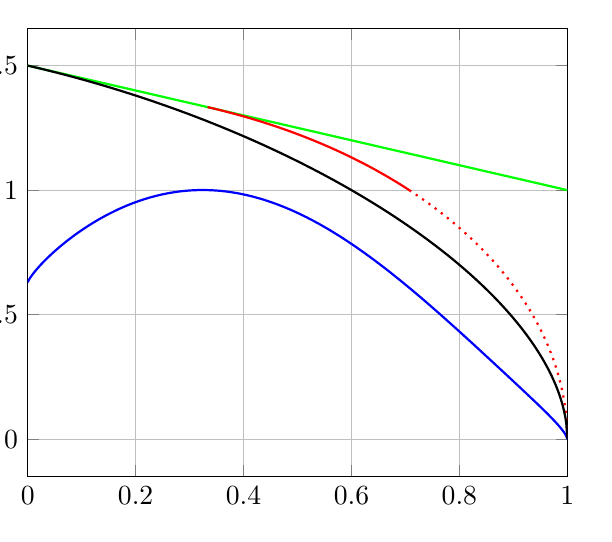
\begin{tikzpicture}[trim axis left,
    declare function={entropy(\x) = - \x * ln(\x)/ln(2) - (1 - \x) * ln(1 - \x) / ln(2); },
%    declare function = { entropy(\x) = 1; },
    ]
    \begin{axis}[domain=0:1,
      samples=500,
      enlarge x limits=false,
      grid=both,
      no markers]
      \addplot +[thick,green] {(3 - x)/2};
      \addplot +[thick,domain=(1/3):(1/1.414),red] {sqrt(2 * (1 - x^2))};
      \addplot +[thick,dotted,domain=(1/1.414):1,red] {sqrt(2 * (1 - x^2))};
      \addplot +[thick,blue] { ((1-x)/2)^(2/3) * (1 + x)^(1/3) * 2^(entropy(x)) };

	  \addplot +[thick,black] {(1-x)/2+sqrt(1 - x^2)};	
	  %\addplot +[thick,black, dotted] { sqrt(2) * (1-x)/2+sqrt(1 - x^2)};	
	  %\addplot +[thick,dotted,black] {(3/2)(1+x)^(1/3)(1-x)^(2/3)};	
\end{axis}
  \end{tikzpicture}
  \caption{(Mean) When $\Exp[g(W)]$ grows exponentially, it is instructive to study the scaled quantity $\mu_1(\epsilon) = \sqrt[d]{\Exp[g(W)]}$. The figure shows a graph of the function $\mu_1(\epsilon)$ in blue, along with the upper bounds on $\mu_1()$ discussed above. The black curve is the asymptotic bound from Claim~\ref{claim:t2star-exact}.}
  \label{fig:grinding-power-mean}
\end{figure}

} % end iftoggle{drawfigs}




%===========================================================


In what follows, we develop tighter bounds via the asymptotics of the binomial coefficients.

\paragraph{Asymptotic bounds on $S(d,z)$.} 
When $z \leq d/3$, the sum $S(d,z)$ will contain the central binomial coefficient ${d-z \choose (d-z)/2}$ which is $\Theta(2^{d-z}/\sqrt{d-z})$. 
It follows that 
\begin{equation} \label{eq:S_d_z_small}
    2^{d-z-1} 
    \leq 
    S(d,z)
    \leq 2^{d-z}\,, 
    \qquad \text{if}\quad 0 \leq z \leq d/3 
    \,.
\end{equation}
On the other hand, for any $0 \leq t < N/2$
\begin{align}\label{eq:binomial-sum-bound}
\frac{2^{H(t/N)N} }{\sqrt{8 (t/N) (1-t/N)} }
\leq 
\sum_{k=0}^t{ {N \choose k} } 
&\leq 
2^{H(t/N)N} \, , 
\end{align}
where $H : [0, 1] \rightarrow [0, 1]$ is the binary entropy function defined as
\begin{align*}
    H(0) &= H(1) = 0\, , \\
    H(\alpha) &= -\alpha \log_2(\alpha) - (1-\alpha) \log_2(1-\alpha)\,, 
        \qquad \text{if}\quad 0 < \alpha < 1\, .
\end{align*}
Thus we can bound $S(d,z)$ using (\ref{eq:binomial-sum-bound}) as follows:
\begin{equation} \label{eq:S_d_z_large}
    \frac{2^{(d-z)H(z/(d-z))}(d-z)}{\sqrt{8 z(d-2z) }}
    \leq
    S(d, z) 
    \leq
    2^{(d-z)H(z/(d-z))}
    \,,\qquad \text{if} \quad d/3 < z \leq d/2 
    \,.
\end{equation}


\subsection{Exact asymptotics for the first moment}
\newcommand{\DoverTwo}{\lfloor d/2 \rfloor}
\newcommand{\DoverThree}{d/3}

In what follows, we establish asymptotically tight upper and lower bounds on 
\begin{align}\label{eq:m_z}
m(d,z) 
&\defeq S(d,z) {d \choose z} \left(\frac{1+\epsilon}{1-\epsilon}\right)^{z} \left(\frac{1-\epsilon}{2}\right)^{d} \, .
\end{align}
via Claims~\ref{claim:t1star-exact} and ~\ref{claim:t2star-exact}. These claims immediately lead to bounds on $\Exp[ g(W) ]$ via Proposition~\ref{prop:grinding-power-mean}.
We also recall the following obvious bound from the sum of a geometric progression:
\begin{align}\label{eq:geom-series-bound}
\sum_{d=1}^n{r^d} 
&\leq \frac{r^{n+1}}{r-1} \qquad \text{if}\quad r > 1\, .
\end{align}





\begin{claim}[Bounds on $m(d,z)$ with small $z$]\label{claim:t1star-exact}
\[
\phi(\epsilon)^d \frac{3}{4\sqrt{d}}
\leq 
m(d, z) 
\leq \phi(\epsilon)^d
\qquad \text{if}\quad z \leq d/3 \quad \text{and}\quad d\geq 2
\]
where $m(d, z)$ is defined in (\ref{eq:m_z}). 
% Moreover, 
% \[
% m(d, z) \leq 1
% \qquad \text{if}\quad z \geq 2\quad \text{and}\quad \epsilon \geq 0.6\,.
% \]
\end{claim}

\begin{proof}
When $z \leq \DoverThree$, we use the upper bound on $S(d,z)$ from (\ref{eq:S_d_z_small}) in (\ref{eq:m_z}) and get
\begin{align*}
m(z)
&\leq 2^{d-z} {d \choose z} \left(\frac{1+\epsilon}{1-\epsilon}\right)^{z} \left(\frac{1-\epsilon}{2}\right)^{d} \\
&= {d \choose z} \left(\frac{1+\epsilon}{2(1-\epsilon)}\right)^{z} (1-\epsilon)^d\,.
\end{align*}
For $z+1 \leq \DoverThree$, the ratio 
\[
\frac{m(z+1)}{m(z)} 
= \frac{d-z}{z+1} \frac{1+\epsilon}{2(1-\epsilon)}
\geq \underbrace{\frac{d-d/3}{\DoverThree}}_{\geq 2} \underbrace{\frac{1+\epsilon}{2(1-\epsilon)}}_{\geq 1/2}
\geq 1\, .
\]
It follows that the sequence $\{m(z)\}$ is an increasing sequence. Consequently,
\begin{align}
m(z; z \leq \DoverThree)
&\leq m(\DoverThree) \nonumber \\
&= {d \choose \DoverThree} (1+\epsilon)^{\DoverThree} (1-\epsilon)^{d- \DoverThree}2^{-\DoverThree} \nonumber \\
&\leq \frac{2^{d H(1/3)}}{\sqrt{\pi (d/3) (2/3)}} 2^{-d/3} (1+\epsilon)^{d/3} (1-\epsilon)^{2d/3} \nonumber \\
&= \left(2^{H(1/3)-1/3} (1+\epsilon)^{1/3} (1-\epsilon)^{2/3} \right)^d \frac{3}{\sqrt{2 \pi d}} \nonumber \\
&= \phi(\epsilon)^d \frac{3}{\sqrt{2 \pi d}} \nonumber \\
&\leq \phi(\epsilon)^d \frac{6}{\sqrt{5 d}} \, . \label{eq:t1star-q1}
\end{align}
Here, we have used Corollary~\ref{coro:nchoosek_1}, the fact that $H(1/3) - 1/3 = \log_2(3/2)$, and (\ref{eq:phi_eps}). This proves the upper bound of the claim. 

% Additionally, since
% \begin{align*}
% \phi(\epsilon) 
% &\defeq \frac{3}{2} (1+\epsilon)^{1/3}(1-\epsilon)^{2/3} \\
% &= \frac{3}{2} \left( (1-\epsilon^2)(1-\epsilon) \right)^{1/3} \\
% &= \frac{3}{2} \left( 1-\epsilon - \epsilon^2 + \epsilon^3 \right)^{1/3} \\
% &= \frac{3}{2}\left( 
% 1 
% + \frac{1}{3}( -\epsilon - \epsilon^2 + \epsilon^3) 
% + \frac{-1}{18}( -\epsilon - \epsilon^2 + \epsilon^3)^2
% + \cdots 
% \right)\\
% &= \frac{3}{2} -\frac{\epsilon}{2} -\left(\frac{1}{2} + \frac{1}{12} \right)\epsilon^2 + O(\epsilon^3) \, ,
% \end{align*}
% $\phi(\epsilon)$ decreases monotonically as $\epsilon$ increases. Hence
% \[
% \phi(\epsilon)\bigg\rvert_{\epsilon \geq 0.6}
% \leq \phi(0.6)
% = \frac{3}{2} (1.6)^{1/3}(0.4)^{2/3}
% = \frac{3}{2}4^{1/3}\frac{4}{10}
% = \frac{3\cdot 4^{1/3}}{5}
% \leq 0.96 < 1\, .
% \]
% This proves the ``moreover'' part of the claim. 

For the lower bound on $m(z)$, apply the lower bound ${N \choose \alpha N} \geq 2^{H(\alpha)N}/\sqrt{8N\alpha (1-\alpha)}$ from Corollary~\ref{coro:nchoosek_1} to the exact expression of $m( \DoverThree)$. This gives 
\begin{align*}
m( \lfloor \DoverThree \rfloor )
&= {d \choose d/3} 
(1+\epsilon)^{d/3} 
(1-\epsilon)^{2d/3} 
2^{-d/3} \nonumber \\
&\geq \frac{2^{d H(1/3)}}{\sqrt{8(d/3)(2/3)}} 2^{-d/3} 
(1+\epsilon)^{d/3} 
(1-\epsilon)^{2d/3} 
\nonumber \quad \text{using Corollary~\ref{coro:nchoosek_1} } \\
&= \frac{3}{4\sqrt{d}}\left(2^{H(1/3) - 1/3} (1+\epsilon)^{1/3} (1-\epsilon)^{2/3}\right)^d \nonumber \\
&= \frac{3}{4\sqrt{d}}\left(\frac{3}{2} (1+\epsilon)^{1/3} (1-\epsilon)^{2/3}\right)^d \\
&= \frac{3}{4\sqrt{d}}\phi(\epsilon)^d \, .
\end{align*}

\end{proof}







\begin{claim}[Bounds on $m(d,z)$ with large $z$]\label{claim:t2star-exact}
\[
\frac{\gamma(\epsilon)^d}{2d}
\leq
m(d, z) 
\leq
\gamma(\epsilon)^d 
% \frac{3\sqrt{d}}{8}
\qquad \text{if}\quad \frac{d}{3} < z \leq \DoverTwo
\, .
\]
where $m(d, z)$ is defined in (\ref{eq:m_z}) and $\gamma(\epsilon) \defeq (1-\epsilon)/2 + \sqrt{1-\epsilon^2}$. Moreover, 
\[
m(d, z) \leq 1
\qquad \text{if}\quad \epsilon \geq 0.6\,.
\]
\end{claim}

\begin{proof}
\textbf{The upper bound.} When $d/3 < z \leq \DoverTwo$, we use the upper bound on $S(d, z)$ from (\ref{eq:S_d_z_large}) into (\ref{eq:m_z}) to get
\begin{align*}
m(z) 
&\leq 2^{(d-z)H(z/(d- z))} {d \choose z} \left(\frac{1+\epsilon}{1-\epsilon}\right)^{z} \left(\frac{1-\epsilon}{2}\right)^{d} \\
&\leq 2^{(d-z)H(z/(d- z)) + H(z/d) d}\left(\frac{1+\epsilon}{1-\epsilon}\right)^{z} \left(\frac{1-\epsilon}{2}\right)^{d}
\end{align*}
using the asymptotic approximation ${N\choose k} \leq 2^{H(k/N)N}$ for $k \leq N/2$. For a fixed $\epsilon$, the function at the exponent of two is concave. There must be some $z^* \in (d/3, \DoverTwo]$ which maximizes $m(z)$. We continue developing the upper bound by setting $\alpha \defeq z/d$. 
\begin{align}
m(z) 
&\leq \left( 2^{q(\alpha, \epsilon)}\right)^d \label{eq:t2star-q2}
\end{align}
where we have defined
\begin{align} \label{eq:q2}
q(\alpha, \epsilon)
& \defeq (1-\alpha) H\left( \frac{\alpha}{1-\alpha} \right) +
H(\alpha) 
-1  + \alpha \log \frac{1+\epsilon}{1-\epsilon} + \log (1-\epsilon)
\end{align}
and $\log$ denotes the base-$2$ logarithm. By applying the definition of $H(.)$,
\begin{align}\label{eq:q2-expanded}
q(\alpha, \epsilon)
&= (1-\alpha) \log\left[
\left( \frac{1-\alpha}{\alpha} \right)^{\frac{\alpha}{1-\alpha} }
\left(\frac{1-\alpha}{1-2\alpha} \right)^{\frac{1-2\alpha}{1-\alpha} }\right] \nonumber \\
& \quad+ \log \left(\frac{1}{\alpha}\right)^\alpha \left(\frac{1}{1-\alpha}\right)^{1-\alpha} \nonumber \\
& \quad+ \log \left(\frac{1+\epsilon}{1-\epsilon}\right)^\alpha + \log(1-\epsilon) -1 \nonumber \\
&= -\log \left[ 
\alpha^{2\alpha} 
(1-2\alpha)^{1-2\alpha} 
\cdot \left(\frac{1-\epsilon}{1+\epsilon}\right)^\alpha 
\right] + \log(1-\epsilon) - 1\, .
% &= 2 a \log(1-2 a)-2 a \log(a)-a \log(1-\epsilon)+\log((-1+\epsilon)/(-2+4 a))+a \log(1+\epsilon)
\end{align}
For a fixed $\epsilon$, this is a unimodal concave function in $\alpha$. The first derivatives of $q(\alpha, \epsilon)$ is
\begin{align*}
\frac{\partial q(\alpha, \epsilon)}{\partial \alpha}
&= \log\left[ \frac{(1-2\alpha)^2}{\alpha^2} \frac{1+\epsilon}{1-\epsilon} \right]
\end{align*}
By setting the above derivative to zero, we find that $q(\alpha, \epsilon)$ is maximized at 
\[
\alpha^* \defeq \alpha^*(\epsilon) 
= \frac{1}{2+\sqrt{\frac{1-\epsilon}{1+\epsilon}} }
= \frac{1}{2+1/r_\epsilon }
= \frac{r_\epsilon}{1 + 2 r_\epsilon }
\]
where we define $r_\epsilon^2 \defeq (1+\epsilon)/(1-\epsilon)$. This means $1-2\alpha = 1/(1+2 r_\epsilon)$. Substituting $\alpha = \alpha^*$ in (\ref{eq:q2-expanded}),
\begin{align*} 
q^*(\epsilon) 
&\defeq q(\alpha^*, \epsilon) \\
&= - \log\left[
\left(\frac{r_\epsilon}{1 + 2 r_\epsilon }\right)^\frac{2 r_\epsilon}{1+2 r_\epsilon}
\left(\frac{1}{1+2r_\epsilon}\right)^\frac{1}{1+2 r_\epsilon}
\cdot \left(\frac{1}{r_\epsilon^2}\right)^\frac{r_\epsilon}{1+2 r_\epsilon}
\right] + \log (1-\epsilon) - 1 \nonumber \\
&= - \log\left[
\frac{1}{1+2 r_\epsilon}
\right] - \log (1-\epsilon) - 1 \nonumber \\
&= \log\frac{1 + 2 r_\epsilon}{1-\epsilon} - 1 \nonumber \\
&= \log\left[\left(1 + 2 \sqrt{\frac{1+\epsilon}{1-\epsilon} } \right) (1-\epsilon) \right] - 1 \nonumber \\
&= \log\left( 1-\epsilon + 2\sqrt{1-\epsilon^2}\right) - 1 \nonumber \\
\implies 2^{q^*(\epsilon)}
&= \frac{1-\epsilon}{2} + \sqrt{1-\epsilon^2}\, .
\end{align*}
This proves the upper bound of the claim. In particular, the derivative of $q^*(\epsilon)$ with respect to $\epsilon$ is $-1/2 - \epsilon/\sqrt{1-\epsilon^2}$. This derivative is negative for all $\epsilon$. Considering that $q^*(0.6) = 1$, it follows that $q^*(\epsilon) < 1$ when $\epsilon > 0.6$. This proves the ``moreover'' part of the claim.

\textbf{The lower bound.} We can use the lower bound on $S(d, z)$ from (\ref{eq:S_d_z_large}) into (\ref{eq:m_z}) to get
\begin{align*}
m(z) 
&\geq 2^{(d-z)H(z/(d- z))}\frac{(d-z)}{\sqrt{8z(d-2z)}} 
{d \choose z} \left(\frac{1+\epsilon}{1-\epsilon}\right)^{z} 
\left(\frac{1-\epsilon}{2}\right)^{d} \\
&\geq 2^{(d-z)H(z/(d- z))}\frac{(d-z)}{\sqrt{8z(d-2z)} } \frac{2^{d H(z/d)} \sqrt{d}}{\sqrt{8z(d-z)} }
\left(\frac{1+\epsilon}{1-\epsilon}\right)^{z} \left(\frac{1-\epsilon}{2}\right)^{d} \qquad \text{using Corollary~\ref{coro:nchoosek_1} on }{d \choose z}\\
&= \frac{\sqrt{d} \sqrt{d-z}}{8z\sqrt{(d-2z)} } 
\left( 2^{q(\alpha, \epsilon)}\right)^{d} \qquad \text{using}\quad \alpha = z/d \quad \text{and} \quad q(\alpha, \epsilon) \text{ from (\ref{eq:q2}) }\\
&= \frac{\sqrt{1-\alpha}}{8\alpha \sqrt{d} \sqrt{(1-2\alpha)} } 
\left( 2^{q(\alpha, \epsilon)}\right)^{d} \\
&\geq \frac{1}{2\sqrt{d}} 
\left( 2^{q(\alpha, \epsilon)}\right)^{d} \qquad \text{since}\quad 1/3 \leq \alpha \leq 1/2\, .
\end{align*}
We have already seen that the right hand side will be maximized by setting
\[
2^{q(\alpha, \epsilon)} \leq \frac{1-\epsilon}{2} + \sqrt{1-\epsilon^2} \qquad \text{for} 1/3 \leq \alpha \leq 1/2, .
\]
This proves the lower bound in the claim.
\end{proof}




% Now we are ready to prove Proposition~\ref{prop:grinding-power-mean}.
% % \restatePropMeanBounds*
% \begin{proof}
% First, note that (\ref{eq:grinding-power-mean-sum}) and (\ref{eq:m_z}) imply that $\Exp[g(W)] = \sum_{d=1}^n{m(d,z)}$. Next, we combine the upper bounds from Claims~\ref{claim:t1star-exact} and \ref{claim:t2star-exact} as $m(d,z) \leq \gamma(\epsilon)^d$ since $\phi(\epsilon) \leq \gamma(\epsilon)$ for $0 \leq \epsilon \leq 1$. This gives $\Exp[ g(W) ] \leq \sum_{d=1}^n{\gamma(\epsilon)^d}$. This is a geometric series; the inequality (\ref{eq:geom-series-bound}) gives the desired upper bound when $\epsilon < 0.6$. At $\epsilon = 0.6$, $\gamma(\epsilon) = 1$; this gives the upper bound of $n$. When $\epsilon > 0.6$, the upper bound is obtained from the geometric-series bound by observing that $\gamma(\epsilon) < 1$.

% The lower bounds for $\epsilon \neq 0.6$ are obtained by summing the geometric series corresponding to the lower bounds from Claims~\ref{claim:t1star-exact} and \ref{claim:t2star-exact}. When $\epsilon = 0.6$, $\gamma(\epsilon) = 1$ and the lower bound is $\sum_{d=1}^n{(1/2d)}$; this equals $1/2$ times the $n$th Harmonic number which, in turn, is at least $\log_e n$. 

% \end{proof}
%--------------------------------------------











% Now we are ready to prove Proposition~\ref{prop:grinding-power-second-moment}
% % \restatePropSecondMomentBounds*
% \begin{proof}
% Recall the inequality $\sum_{d=1}^n{r^d} \leq r^{n+1}/(r-1) = r^n\cdot r/(r-1)$ which follows from the geometric series with $r > 1$. The bounds are obtained by applying this inequality to the upper bounds in Claim~\ref{claim:t1star-variance-exact} and Claim~\ref{claim:t2star-variance-exact}, then making the following observations.
% \begin{align*}
% \frac{5-3 \epsilon}{3-3\epsilon} 
% &\leq 2 \qquad \text{if}\qquad 0 \leq \epsilon \leq 1/3 \\
% \frac{2^{2/3} \phi(\epsilon)}{2^{2/3} \phi(\epsilon) - 1} 
% &\leq 3 \qquad \text{if}\qquad 1/3 < \epsilon \leq 0.6 \\
% \end{align*}

% The last bound follows directly from Claim~\ref{claim:t2star-variance-exact}.
% \end{proof}







%============================================



\subsection{Exact asymptotics for higher moments}
\begin{proposition}\label{prop:grinding-power-moment}
For $t \in \mathbb{N}, t \geq 2$,
\[
\Exp[ g(W)^t ] 
\leq 
(n+3)\left[\frac{1}{2}\left( 2^t + 1 - \epsilon (2^t -1) \right)\right]^n 
\qquad \text{if} \qquad \epsilon \leq \frac{2^t - 2}{2^t + 2}\, .
\]
\end{proposition}
\begin{proof}
Observe that
\begin{align*}
\Exp[ g(W)^t ]
&= \sum_{d = 1}^n{ \Exp[ g(W_{n-d+1}, \cdots, W_n)^t ] }\, ,
\end{align*}
and
\begin{align*}
\Exp[ g(W_{n-d+1}, \cdots, W_n)^t ] 
&= \sum_{z = 0}^{\lfloor d/2 \rfloor} {S(d,z)^t  B(d, (1-\epsilon)/2; z) } \, .
% &= \sum_{z=0}^{\lfloor d/2 \rfloor} {S(d,z)^t {d \choose z} \left(\frac{1+\epsilon}{1-\epsilon}\right)^{z} \left(\frac{1-\epsilon}{2}\right)^{d} }\, .
\end{align*}
Following our own footsteps in arriving at (\ref{eq:q2}), we can write
\begin{align*}
\Exp[ g(W_{n-d+1}, \cdots, W_n)^t ] 
&\leq \sum_{\alpha=0}^{1/3}{2^{t(d-z)} B(d, (1-\epsilon)/2; z) } 
+ \sum_{\alpha=1/3}^{1/2}{2^{t(d-z)H(z/(d-z))} B(d, (1-\epsilon)/2; z) } \\
&= \sum_{\alpha=0}^{1/3}{2^{q_1(\alpha, \epsilon, t)d}} 
+ \sum_{\alpha=1/3}^{1/2}{2^{q_2(\alpha, \epsilon, t)d}} \, ,
\end{align*}
where we have defined
\begin{align} 
q_1(\alpha, \epsilon, t)
& \defeq t(1-\alpha) +
H(\alpha) 
-1  + \alpha \log \frac{1+\epsilon}{1-\epsilon} + \log (1-\epsilon) \label{eq:q1t} \, ,\\
q_2(\alpha, \epsilon, t)
& \defeq t(1-\alpha) H\left( \frac{\alpha}{1-\alpha} \right) +
H(\alpha) 
-1  + \alpha \log \frac{1+\epsilon}{1-\epsilon} + \log (1-\epsilon) \label{eq:q2t}\, .
\end{align}
We calculate the derivatives:
\begin{align*}
\frac{\partial q_1(\alpha, \epsilon, t)}{\partial \alpha}
&= -t 
+ \log \frac{1-\alpha}{\alpha}
+ \log \frac{1+\epsilon}{1-\epsilon} \, ,
\\
\frac{\partial q_1(\alpha, \epsilon, t)}{\partial \alpha}
&= 
(1+t) \log \frac{1-\alpha}{\alpha} 
+ 2 t \log \frac{1 - 2 \alpha}{1 - \alpha}
+ \log \frac{1+\epsilon}{1-\epsilon} \, .
\end{align*}
We observe that $q_1()$ and $q_2()$ agree at $\alpha = 1/3$, as do their derivatives. That is,
\begin{align*}
&q_1(1/3, \epsilon, t) = q_2(1/3, \epsilon, t) \, , \qquad \text{and}\\
&\frac{\partial q_1(\alpha, \epsilon, t)}{\partial \alpha}\bigg\rvert_{\alpha = 1/3}
=
\frac{\partial q_2(\alpha, \epsilon, t)}{\partial \alpha}\bigg\rvert_{\alpha = 1/3}
= 
1 - t + \log \frac{1+\epsilon}{1-\epsilon} \, .
\end{align*}
In addition, $\partial q_1/\partial \alpha$ -- and by equality, $\partial q_2/\partial \alpha$  -- will be non-positive if and only if
\begin{align}
&\epsilon \leq \epsilon^*(t) \defeq \frac{2^t - 2}{2^t + 2} \label{eq:epsstar-moment}
\, .
\end{align}
Notice that we need $t \geq 2$ for $\epsilon^*(t)$ to be meaningful. 

Next, observe that $q_1(\alpha, \epsilon, t)$ is concave in $\alpha$. Suppose $\alpha = \alpha^*$ maximizes $q_1()$. Then, it follows that $q_1(\alpha^*, \epsilon, t) \geq q_1(1/3, \epsilon, t) = q_2(1/3, \epsilon, t) \geq q2(\alpha, \epsilon, t)$. The last inequality follows from the two following facts: that $\partial q_2/\partial \alpha$ is non-positive at $\alpha = 1/3$ and that $q_2()$ is concave in $\alpha$. We can directly solve for $\alpha^*$ by writing \[r_\epsilon \defeq \frac{1+\epsilon}{1-\epsilon}\] and setting
\begin{align*}
&\frac{\partial q_1(\alpha, \epsilon, t)}{\partial \alpha} = 0 \\
\implies& -t 
+ \log \frac{1-\alpha}{\alpha}
+ \log r_\epsilon
=0 \\
\implies& \alpha^* = \frac{1}{1+\frac{2^t}{r_\epsilon}}\, .
\end{align*}
Plugging in $\alpha = \alpha^*$ in (\ref{eq:q1t}), we get
\begin{align*}
q_1(\alpha^*, \epsilon, t)
&= \frac{ \frac{2^t}{r_\epsilon}(t - 1 - \log \frac{2^t}{r_\epsilon} ) - 1 + \log r_\epsilon }{1 + \frac{2^t}{r_\epsilon} }
+ \log \left[ (1-\epsilon) (1+\frac{2^t}{r_\epsilon})\right]\\
&= \log \left[2^t + 1 - \epsilon (2^t -1) \right] - 1\, .
\end{align*}
Thus if we set \begin{align*}
s(\epsilon, t) 
&\defeq 2^{q_1(\alpha^*, \epsilon, t)} \\
&= \frac{1}{2}\left( 2^t + 1 - \epsilon (2^t -1) \right)\, ,
\end{align*}
then
\[
\Exp[ g(W_{n-d+1}, \cdots, W_n)^t ] 
\leq
\frac{d}{2} s(\epsilon, t)^d
\qquad
\text{and}
\qquad
\Exp[ g(W)^t ] 
\leq 
\sum_{d=1}^n{\frac{d}{2} s(\epsilon, t)^d}\, .
\]
It is not difficult to see that for $r> 1$,
\[
\sum_{d=1}^n{d r^d} 
= r \cdot \frac{d}{d r} \left[ \sum_{d=1}^n{r^d}\right] 
\leq \frac{d}{d r} \frac{r^{n+1}}{r-1} 
= \frac{r^{n+1}}{r-1} \left( n + 1 + \frac{r}{r-1}\right) \, ,
\]
where the inequality follows from (\ref{eq:geom-series-bound}). Moreover, If we set $r = s(\epsilon, t)$ in the above equation, we have 
\[
\Exp[ g(W)^t ] 
\leq 
\frac{s(\epsilon, t)^{n+1}}{s(\epsilon, t)-1} \left( n + 1 + \frac{s(\epsilon, t)}{s(\epsilon, t)-1}\right)\, .
\]

\begin{claim}\label{claim:s-ratio}
Equation (\ref{eq:epsstar-moment}) implies
\[
\frac{s(\epsilon, t)}{s(\epsilon, t) - 1 } \leq 2\, .
\]
\end{claim}
Postponing a proof of Claim~\ref{claim:s-ratio} for the moment, we observe that the claim immediately leads to a proof of Proposition~\ref{prop:grinding-power-moment}:
\begin{align*}
\Exp[ g(W)^t ] 
&\leq \sum_{d=1}^n{\frac{d}{2} s(\epsilon, t)^d}\\
&\leq \frac{1}{2} \left[2 s(\epsilon,t)^n ( n + 3) \right] \\
&= (n+3)\left[\frac{1}{2}\left( 2^t + 1 - \epsilon (2^t -1) \right)\right]^n\, .
\end{align*}
It remains to prove Claim~\ref{claim:s-ratio}. Using (\ref{eq:epsstar-moment}), we get
\begin{align}
\frac{s(\epsilon, t)}{s(\epsilon, t)-1}
&= \frac{2^t + 1 - \epsilon(2^t - 1)}{2^t - 1 - \epsilon(2^t - 1)} \nonumber \\
&= 1 + \frac{2}{2^t - 1 - \epsilon(2^t - 1)} \label{eq:claim-s-ratio}
\, .
\end{align}
However, starting from (\ref{eq:epsstar-moment}) we can see that
\[
\epsilon 
\leq 
\frac{2^t - 2}{2^t +2} 
\leq 
\frac{2^t - 5}{2^t - 1}
\leq
\frac{2^t - 3}{2^t - 1}\, .
\]
The last inequality is equivalent to saying $\epsilon(2^t - 1) \leq 2^t - 3$, or $2^t - 1 -\epsilon(2^t - 1) \geq 2$. Referring back to (\ref{eq:claim-s-ratio}), this implies $\displaystyle \frac{s(\epsilon, t)}{s(\epsilon, t)-1} \leq 2$. The proof of Claim~\ref{claim:s-ratio} follows, completing the proof of Proposition~\ref{prop:grinding-power-moment}.
\end{proof}


%------------------- Variance, z > d/3, eps > 0.6 ----------------------
% \textbf{When $\epsilon$ is large.}
% Now consider the case $\epsilon > 0.6$. Setting $\alpha \defeq z/d$ and using the upper bounds from Corollaries ~\ref{coro:nchoosek_1} and \ref{coro:nchoosek_2}, we get
% \begin{align*}
% n(z)
% &\leq a_z \\
% &= 2^{-d}
% (1-\epsilon)^d 
% (d - 2z)^2 
% {d-z \choose z}^2 
% {d \choose z} 
% \left(\frac{1+\epsilon}{(1-\epsilon)}\right)^{z} \\
% &\leq 
% 2^{-d} 
% d^2 
% (1-2\alpha)^2
% 2^{2(1-\alpha)dH(\alpha/(1-\alpha))} \left(\frac{1-\alpha}{\pi d \alpha (1-2\alpha)} \right)
% \frac{2^{H(\alpha)d}}{\sqrt{\pi d \alpha(1-\alpha)}}
% \left(\frac{1+\epsilon}{1-\epsilon}\right)^{\alpha d} (1-\epsilon)^d \\
% &= \frac{\sqrt{d}(1-2\alpha)\sqrt{1-\alpha}}{\pi \alpha \sqrt{\pi \alpha}}
% \left( 2^{H(\alpha) - 1 + 2(1-\alpha) H\left(\alpha/(1-\alpha)\right)} 
% \left(\frac{1+\epsilon}{1-\epsilon}\right)^{\alpha} (1-\epsilon) 
% \right)^d \\
% &\leq \frac{\sqrt{d} }{3} \left( 2^{q(\alpha, \epsilon)} \right)^d\, ,
% \end{align*}
% where
% \begin{align*}
% q(\alpha, \epsilon)
% &\defeq H(\alpha) - 1 + 2(1-\alpha) H\left(\frac{\alpha}{1-\alpha}\right) 
% + \alpha \log \frac{1+\epsilon}{1-\epsilon}+\log(1-\epsilon)\,.
% \end{align*}
% Observe that $q(\alpha, \epsilon)$ is concave in $\alpha$ since for a fixed $\epsilon$, it is a linear combination of the concave entropy function and $\alpha$. The derivatives of $q(\alpha, \epsilon)$, with respect to $\alpha$, are as follows:
% \begin{align*}
% \frac{\partial}{\partial \alpha}q(\alpha, \epsilon)
% &= \log \left(\frac{(1-2\alpha)^4}{\alpha^3(1-\alpha)}  \frac{1+\epsilon}{1-\epsilon} \right)\, .\\
% % \frac{\partial^2}{\partial \alpha^2}q(\alpha, \epsilon)
% % &= -\frac{3-2\alpha}{\alpha(1+2\alpha^2 -3\alpha)} \\
% % \frac{\partial^3}{\partial \alpha^3}q(\alpha, \epsilon)
% % &= \frac{3-2\alpha( 3-2\alpha)^2}{\alpha^2(1+2\alpha^2 -3\alpha)^2} < 0\, .
% \end{align*}

%===========================================================
\subsection{Stirling's approximation and binomial coefficients}
Let us briefly recall an upper bound on binomial coefficients.

\begin{theorem}[Stirling's approximation]
For any positive integer $n$,
\[
n! \, = \, \sqrt{2\pi n}(\frac{n}{e})^n e^{r(n)}\, ,
\]where
\[
\frac{1}{12n} < r(n) < \frac{1}{12n + 1}.
\]
\end{theorem}

Let the binary entropy function $H : [0, 1] \rightarrow [0, 1]$ be defined as
\begin{align*}
H(\alpha) & \defeq \left\{ \begin{array}{ll}0 & \text{ if } \alpha \in \{0, 1\}\\
\\
-\alpha \log_2(\alpha) - (1-\alpha) \log_2(1-\alpha) & \text{ if } \alpha \in (0, 1)\end{array} \right. .
\end{align*}

\begin{corollary}\label{coro:nchoosek_1}
For a positive integer $n$ and any $\alpha \in \{\frac{1}{n}, \frac{2}{n}, \cdots, \frac{1}{2} \}$, 
\begin{align}\label{eq:nck}
  \frac{2^{n H(\alpha)}}{\sqrt{8 n\alpha (1-\alpha)}} 
  \leq {n \choose \alpha n} 
  \leq \frac{2^{n H(\alpha)}}{\sqrt{\pi n\alpha (1-\alpha)}} 
  \leq \frac{2^{n H(\alpha)}}{\sqrt{\pi/2}} \, .
\end{align}
\end{corollary}

\begin{proof}
\begin{align*}
{n \choose \alpha n}
&= \frac{n!}{(\alpha n)!\, \left( (1-\alpha)n \right)! }\\
&\approx \frac{\sqrt{2\pi n}(\frac{n}{e})^n}{2\pi n\sqrt{\alpha (1-\alpha)}(\frac{\alpha n}{e})^{\alpha n}(\frac{(1-\alpha)n}{e})^{(1-\alpha)n} } \underbrace{ \exp\left( \frac{1}{12n} - \frac{1}{12\alpha n + 1} - \frac{1}{12(1-\alpha)n+1}\right) }_{ E(n,\alpha) } \\
&= 2^{n H(\alpha)} \, 1/\underbrace{ \sqrt{2 \pi n\alpha (1-\alpha)} }_{F(n, \alpha)} \, E(n, \alpha) \\
&=2^{n H(\alpha)} E(n, \alpha)/F(n, \alpha) \, .
\end{align*}

\emph{(The upper bounds.)} $E(n,\alpha)$ is at most $e^{1/12 n} < \sqrt{2}$. Hence the first (tighter) upper bound follows. Now we deal with the quantity $F(n, \alpha)/\sqrt{2} = \sqrt{\pi n \alpha (1-\alpha)}$. Since $1-\alpha \geq 1/2$ and $\alpha \geq 1/n$, we have this is at least $ \sqrt{\pi/2}$. \emph{(The lower bound.)} $E(n, \alpha)$ is at least $1$, and $2\pi$ is at most $8$. Hence the bound follows.

\end{proof}

\begin{corollary}\label{coro:nchoosek_2}
For a positive integer $n$ and any $\alpha \in [\frac{1}{n},\frac{1}{2} - \frac{1}{n}]$, 
\begin{align}\label{eq:nck_2}
{(1-\alpha)n \choose \alpha n} \leq 2^{(1-\alpha)n\,H\left( \frac{\alpha}{1-\alpha} \right)}\, G(n, \alpha)\,,
\end{align}
where \[
 G(n,\alpha) \leq \sqrt{\frac{1-\alpha}{\alpha(1-2\alpha) \pi n} } \leq \sqrt{\frac{1-\alpha}{ 2 \pi \alpha} } \leq \sqrt{ \frac{n-1}{2 \pi} }\, . 
 \]
\end{corollary}
\begin{proof}

\begin{align*}
{(1-\alpha)n \choose \alpha n}
&= \frac{((1-\alpha)n)!}{(\alpha n)!\, \left( (1-2\alpha)n \right)! }\\
&\approx \frac{\sqrt{2\pi (1-\alpha)n}(\frac{(1-\alpha)n}{e})^{(1-\alpha)n}}{2\pi n\sqrt{\alpha (1-2\alpha)}(\frac{\alpha n}{e})^{\alpha n}(\frac{(1-2\alpha)n}{e})^{(1-2\alpha)n} } \underbrace{ \exp\left( \frac{1}{12(1-\alpha)n} - \frac{1}{12\alpha n + 1} - \frac{1}{12(1-2\alpha)n+1}\right) }_{E(n,\alpha)}  \\
&= \underbrace{ \sqrt{\frac{1-\alpha}{\alpha(1-2\alpha) 2 \pi n} } }_{F(n, \alpha)}\, \left( \frac{(1-\alpha)^{1-\alpha}}{\alpha^\alpha (1-2\alpha)^{1-2\alpha}} \right)^n\, E(n, \alpha)\\
&=F(n, \alpha) \, 2^{(1-\alpha)n\,H\left( \frac{\alpha}{1-\alpha} \right)} \, E(n, \alpha)\, .
\end{align*}

First, note that $\alpha \leq 1/2 - 1/n$ implies $(1-2\alpha)n \geq 2$. Consequently, $F(n, \alpha) \leq \sqrt{\frac{1-\alpha}{ 4 \pi \alpha} }$. Moreover, $E(n,\alpha)$ is at most $e^{1/12(1-\alpha)n} < \sqrt{2}$. This gives $F(n, \alpha)E(n, \alpha) \leq \sqrt{\frac{1-\alpha}{ 2 \pi \alpha} }$. Since $\alpha \geq 1/n$, the quantity inside the square root is at most $(1-1/n)/2 \pi(1/n) = (n-1)/2\pi$.

\end{proof}




% \section{XOR games under geometric distribution}
% \label{app:xor-games-geometric}
% \input{tex/xor-games-geometric.tex}



% The figure+table appears in exact-probabilities.tex
%\newpage
%\section{Graphs and tables of exact probabilities}
%\label{app:probabilities}
%\input{exact-app.tex}

\end{document}

%%% Local Variables:
%%% mode: latex
%%% TeX-master: t
%%% End:
